\graphicspath{{./chapters/chapter3/}}

\chapter{Differentially Private Triangle and 4-Cycle Counting in the Shuffle Model}\label{chap:3}

\newcommand{\MSE}{\operatorname{\textsf{MSE}}}

% \def\AlgWS{\textsf{WShuffle}$_{i,j}$}
\def\AlgWS{\textsf{WS}}
\def\AlgWSLE{\textsf{WSLE}}
\def\AlgWSTri{\textsf{WShuffle}$_{\triangle}$}
% \def\AlgWSTri{\textsf{WSLE}$_{\triangle}$}
\def\AlgWSTriVR{\textsf{WShuffle}$_{\triangle}^*$}
% \def\AlgWSTriVR{\textsf{WSLE}$_{\triangle}^*$}

\def\AlgWLTri{\textsf{WLocal}$_{\triangle}$}
\def\AlgARRTri{\textsf{ARR}$_{\triangle}$}
\def\AlgRRTri{\textsf{RR}$_{\triangle}$}
\def\AlgTwoRL{\textsf{2R-Large}$_{\triangle}$}
\def\AlgTwoRS{\textsf{2R-Small}$_{\triangle}$}

\def\AlgWSCyc{\textsf{WShuffle}$_{\square}$}
\def\AlgWLCyc{\textsf{WLocal}$_{\square}$}


\section{Introduction}
\label{chap3-sec:intro}
Graph statistics is useful for finding meaningful connection patterns in network data, and 
% counting subgraphs (e.g., triangles, $k$-stars, cycles, cliques) 
subgraph counting is known as a fundamental task in graph analysis. 
For example, a triangle is a cycle of size three, 
% consists of three nodes with three edges, 
and a $k$-star consists of a central node connected to $k$ other nodes.  
These subgraphs 
% important because they 
can be used to calculate 
a 
% (global) 
clustering coefficient ($=\frac{3 \times \text{\#triangles}}{\text{\#2-stars}}$). 
In a social graph, the clustering coefficient measures 
the tendency of nodes (users) to form a cluster with each other. 
% the degree to which nodes (users) tend to cluster together 
It also represents the average probability that a friend's friend is also a friend \cite{Newman_PRL09}. 
% two friends of a user will also be a friend 
Therefore, the clustering coefficient is useful for analyzing the effectiveness of friend suggestions. 
% For another example, a 4-cycle is a cycle composed of four nodes 
Another example of the subgraph is a 4-cycle, 
% which is a cycle composed of four nodes. 
a cycle of size four. 
The 4-cycle count is useful for measuring the clustering ability in bipartite graphs (e.g., 
% sexual contact networks \cite{Lind_PRE05}) 
online dating networks, mentor-student networks \cite{Kutty_WWW14}) 
where a triangle never appears \cite{Lind_PRE05,Robins_CMOT04,Sanei-Mehri_CIKM19}. 
Figure~\ref{chap3-fig:subgraphs} shows examples of triangles, 2-stars, and 4-cycles. 
% 
% Although subgraph counts are important for analyzing the connection patterns or clustering tendency, they can leak sensitive edges (friendships). 
Although these subgraphs are important for analyzing the connection patterns or clustering tendencies, their exact numbers can leak sensitive edges (friendships) \cite{Imola_USENIX21}. 
%include sensitive data such as sensitive friendships. 
% For example, in Figure~XX, the triangle count 

\begin{figure}[t]
  \centering
  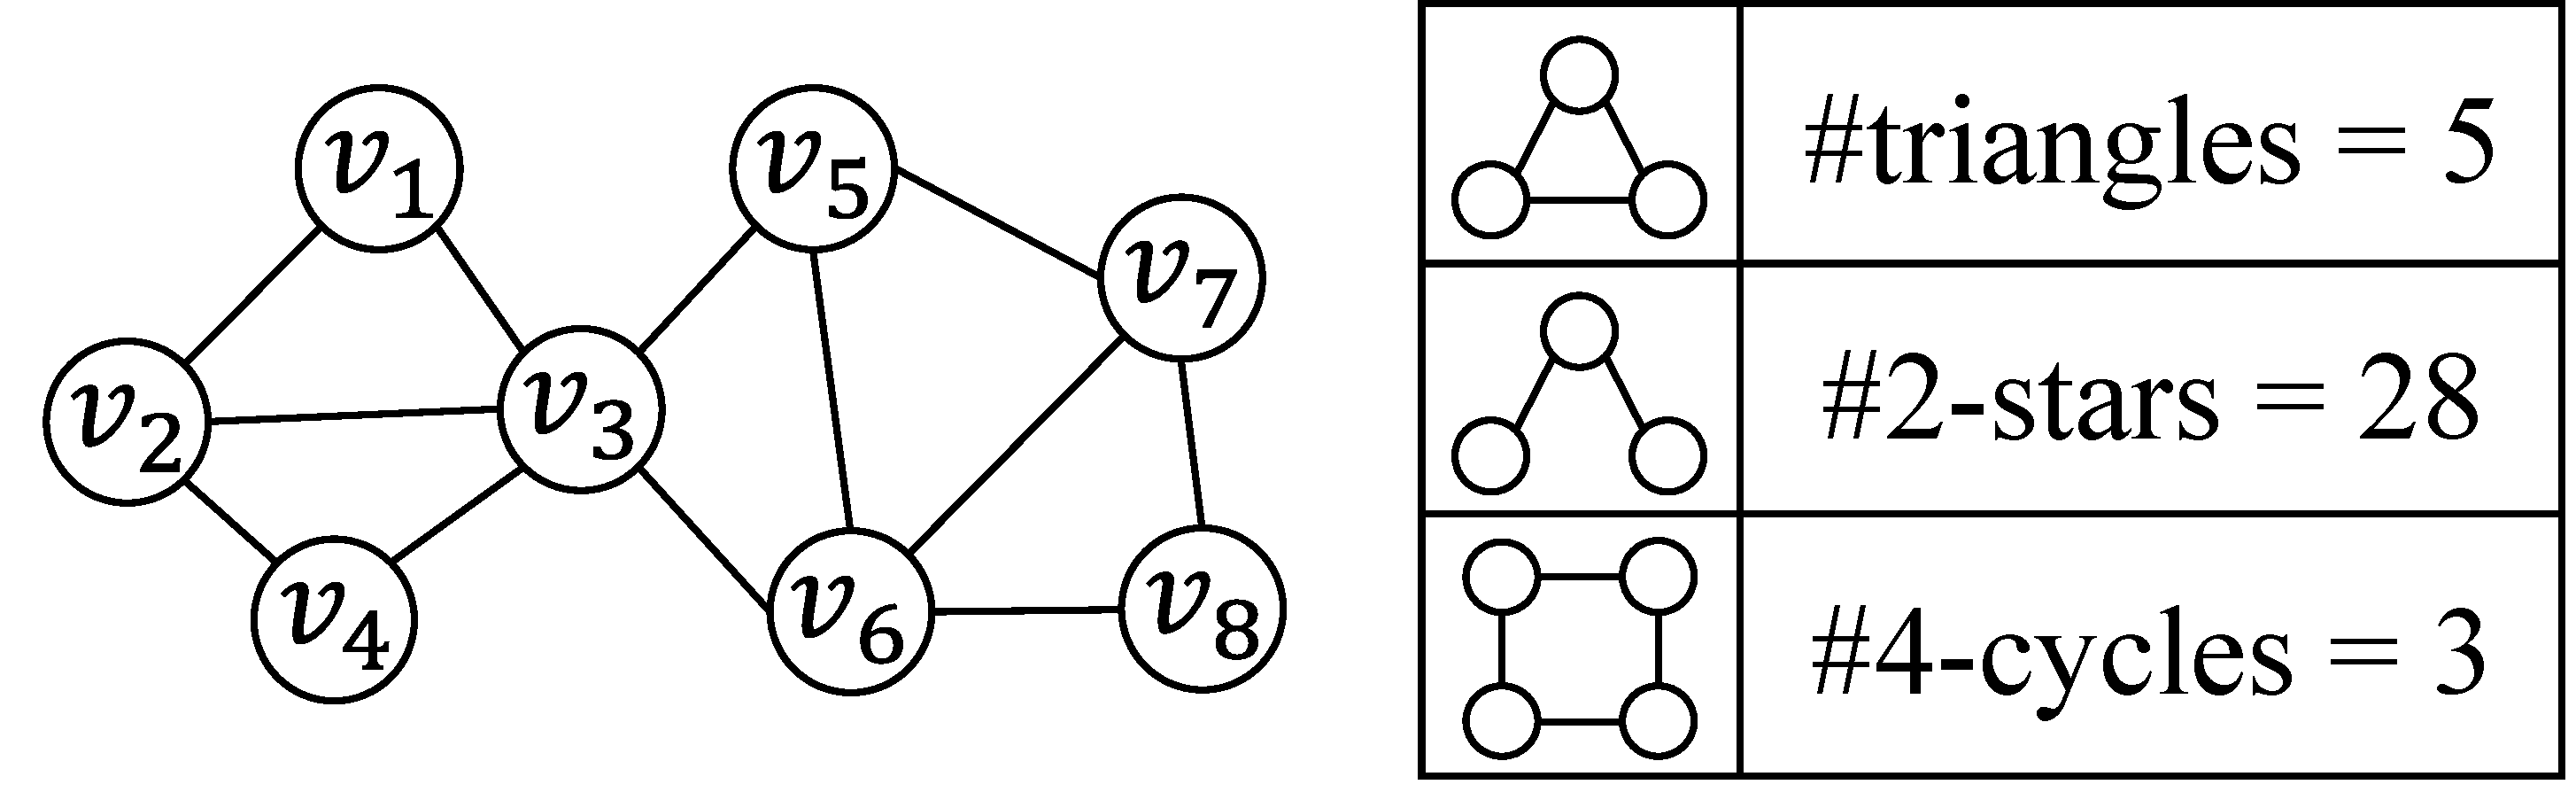
\includegraphics[width=0.65\linewidth]{fig/subgraphs.pdf}
  
  \caption[Examples of subgraph counts.]{Examples of subgraph counts.
  }
  \label{chap3-fig:subgraphs}
\end{figure}

DP (Differential Privacy) \cite{Dwork_ICALP06,DP} -- the gold standard of privacy notions -- has been widely used to strongly protect edges in graph data \cite{Day_SIGMOD16,Ding_TKDE21,Hay_ICDM09,Imola_USENIX21,Imola_USENIX22,Karwa_PVLDB11,Kasiviswanathan_TCC13,qin2017generating,Sun_CCS19,Ye_ICDE20,Ye_TKDE21}. 
% DP strongly protects user privacy when a parameter (privacy budget) $\epsilon$ is small and is known as the gold standard of privacy notions. 
% against adversaries with any background knowledge. 
In particular, recent studies 
\cite{Imola_USENIX21,Imola_USENIX22,qin2017generating,Ye_ICDE20,Ye_TKDE21} 
% \cite{Imola_USENIX21,Imola_USENIX22,Ye_ICDE20,Ye_TKDE21} 
have applied LDP (Local DP) \cite{Kasiviswanathan_FOCS08} to 
graph data. 
% subgraph counting. 
% where each user has 
%subgraph counting. 
In the graph LDP model, each user obfuscates her neighbor list (friends list) by herself and sends the obfuscated neighbor list to a data collector. 
Then, the data collector estimates graph statistics, such as subgraph counts. 
Compared to central DP where a central server has personal data of all users (i.e., the entire graph), LDP does not have a risk that all personal data are leaked from the server by 
% illegal access 
cyberattacks 
\cite{Henriquez_breach2021} or insider attacks \cite{Kohen_insider_threats}. 
Moreover, LDP can be applied to decentralized social networks \cite{Paul_CN14,Salve_CSR18} (e.g., diaspora* \cite{Diaspora}, Mastodon \cite{Mastodon}) where no server can access the entire graph; e.g., 
the entire graph is distributed across many servers, or no server has any original edges. 
It is reported in \cite{Imola_USENIX21} that $k$-star counts can be accurately estimated in this model. 

However, it is much more challenging to accurately count more complicated subgraphs such as triangles and 4-cycles under LDP. 
The root cause of this is its local property -- a user cannot see edges between others. 
% For example, user $v_3$ knows that there are ten $2$-stars of which she is a center. 
% However, $v_3$ cannot count triangles or 4-cycles including $v_3$, as she cannot see edges between others, e.g., $(v_1,v_2)$ and $(v_2,v_4)$. 
For example, user $v_1$ cannot count triangles or 4-cycles including $v_1$, as she cannot see edges between others, e.g., $(v_2,v_3)$, $(v_2,v_4)$, and $(v_3,v_4)$. 
Therefore, the existing algorithms \cite{Imola_USENIX21,Imola_USENIX22,Ye_ICDE20,Ye_TKDE21} 
obfuscate 
each bit of the neighbor list 
% each user's edges 
rather than the subgraph count by 
% apply 
% Warner's 
the RR (Randomized Response) \cite{Warner_JASA65}, which randomly flips 0/1. 
% with some probability, 
% to each bit of the neighbor list. 
As a result, their algorithms suffer from extremely large estimation errors because it makes all edges noisy. 
% any triangle or 4-cycle. 
% To address this issue, 
Some studies \cite{Imola_USENIX21,Imola_USENIX22} 
significantly improve the accuracy by introducing 
% introduce 
an additional round of interaction between users and the data collector. 
% Their algorithms publish the noisy graph at the first round to enable each user to count her triangles such that only one edge is noisy at the second round. 
% In their algorithms, the data collector publishes the noisy graph at the first round. 
% Specifically, they propose triangle algorithms that publish the noisy graph at the first round 
% so that each user can count her triangles at the second round. 
% Then, at the second round, each user can count her triangles such that only one edge is noisy. 
% because she knows two edges connected to her. 
% Therefore, the accuracy is significantly improved. 
% Thus, the two-rounds algorithms significantly reduce the estimation error. 
However, multi-round interaction may be impractical in many applications, as it requires a lot of user effort and synchronization; 
in  \cite{Imola_USENIX21,Imola_USENIX22}, every user must respond twice, and the data collector must wait for responses from all users 
in each round. 
% to publish the noisy graph. 

In this work, we focus on a \textbf{one-round} of interaction between users and the data collector and propose accurate subgraph counting algorithms by introducing a recently studied privacy model: the \textit{shuffle model} \cite{Erlingsson_SODA19,Feldman_FOCS21}. 
% The shuffle model introduces an intermediate server called the shuffler. 
In the shuffle model, each user sends her (encrypted) obfuscated data to an intermediate server called the shuffler. 
Then, the shuffler randomly shuffles the obfuscated data of all users and sends the shuffled data to the data collector (who decrypts them). 
% It has been proven that 
The shuffling amplifies DP guarantees of the obfuscated data under the assumption that the shuffler and the data collector do not collude with each other. 
Specifically, it is known that DP strongly protects user privacy when a parameter (a.k.a. privacy budget) $\epsilon$ is small, e.g., $\epsilon \leq 1$ \cite{DP_Li}. 
The shuffling significantly reduces $\epsilon$ and therefore significantly improves utility at the same value of $\epsilon$. 
To date, the shuffle model has been successfully applied to tabular data \cite{Meehan_ICLR22,Wang_PVLDB20} and 
% image data 
gradients \cite{Girgis_AISTATS21,Liu_AAAI21} in federated learning. 
We 
%make the first attempt (to our knowledge) to apply the shuffle model to subgraph counting. 
apply the shuffle model to graph data to accurately count subgraphs within one round. 
%one-round subgraph counting to provide a small estimation error. 

% However, it is very challenging to apply the shuffle model to subgraph counting because 
The main challenge in subgraph counting in the shuffle model is that each user's neighbor list is \textit{high-dimensional data}, i.e., $n$-dim binary string where $n$ is the number of users. 
% we cannot use the entire neighbor list as input data. 
Consequently, applying the RR to each bit of the neighbor list, as in the existing work \cite{Imola_USENIX21,Imola_USENIX22,Ye_ICDE20,Ye_TKDE21}, results in an extremely large privacy budget $\epsilon$ even after applying the shuffling (see Section~\ref{chap3-sub:technical} for more details). 

We address this issue by introducing a new, basic technique called \textit{wedge shuffling}. 
In graphs, a wedge between $v_i$ and $v_j$ is defined by a 2-hop path with endpoints $v_i$ and $v_j$. 
% Our wedge shuffle technique obfuscates a wedge (2-hop path) between a specific user-pair. 
% rather than the entire neighbor list. 
For example, in Figure~\ref{chap3-fig:subgraphs}, 
there are two wedges between $v_2$ and $v_3$: $v_2$-$v_1$-$v_3$ and $v_2$-$v_4$-$v_3$. 
In other words, users $v_1$ and $v_4$ have a wedge between $v_2$ and $v_3$, whereas $v_5, \ldots, v_8$ do not. 
Each user obfuscates such wedge information by the RR, and the shuffler randomly shuffles them. 
Because the wedge information (i.e., whether there is a wedge between a specific user-pair) 
is \textit{one-dimensional binary data}, it can be sent with small noise and small $\epsilon$. 
In addition, the wedge is the main component of several subgraphs, such as triangles, 4-cycles, and 3-hop paths \cite{Sun_CCS19}. 
Since the wedge has little noise, we can accurately count these subgraphs based on wedge shuffling. 

We apply wedge shuffling to triangle and 4-cycle counting tasks with several additional techniques. 
For triangles, we first 
%consider a problem of counting 
propose an algorithm that counts triangles involving the user-pair at the endpoints of the wedges by locally sending an edge between the user-pair to the data collector. 
% along with shuffled wedges. 
% to count triangles including the user-pair. 
Then we propose an algorithm to count triangles in the entire graph by sampling disjoint user-pairs, which share no common users (i.e., 
no user falls in two pairs). 
We also propose a technique to reduce the variance of the estimate by ignoring sparse user-pairs, where either of the two users has a very small degree. 
For 4-cycles, we propose an algorithm to calculate an unbiased estimate of the 4-cycle count from that of the wedge count via bias correction. 

% We propose triangle and 4-cycle counting algorithms based on our wedge shuffle technique and show upper bounds on the estimation error for our algorithms. 
We provide upper bounds on the estimation error for our triangle and 4-cycles counting algorithms. 
Through comprehensive evaluation, we show that 
% it is possible to accurately estimate 
our algorithms 
accurately estimate these subgraph counts within one round under the shuffle model. 
% to triangles and 4-cycles. 
% with some additional techniques. 
% Our experimental results show that 

% \begin{itemize}
%     \item shuffle model for graphs?
%     \item define graph shuffle model
%     \item problem: high dim data
%     \item counting triangles/4-cycles
%     \item our approach: dim reduction by wedges
% \end{itemize}


\smallskip
\noindent{\textbf{Our Contributions.}}~~Our contributions are as follows: 
\begin{itemize}
    \item We propose a wedge shuffle technique to enable privacy amplification 
    %in subgraph counting. 
    of graph data. 
    To our knowledge, we are the first to shuffle graph data (see Section~\ref{chap3-sec:related} for more details). 
    %apply the shuffle model to graph data. 
    \item We propose one-round triangle and 4-cycle counting algorithms 
    %with theoretical performance guarantees 
    based on our wedge shuffle technique. 
    %apply wedge shuffling to triangles and 4-cycles. 
    For triangles, we propose three additional techniques: sending local edges, sampling disjoint user-pairs, and variance reduction by ignoring sparse user-pairs. 
    For 4-cycles, we propose a bias correction technique. 
    We show upper bounds on the estimation error for each algorithm. 
    \item We evaluate our algorithms using two real graph datasets. 
    Our experimental results show that our one-round shuffle algorithms 
    significantly outperform one-round local algorithms in terms of accuracy 
    %dramatically the estimation error of the one-round local algorithms 
    and achieve a small estimation error (relative error $\ll 1$) with a reasonable privacy budget, e.g., smaller than $1$ in edge DP. 
\end{itemize}
In \conference{the full version of this paper \cite{Imola_CCSFull22}}\arxiv{Appendix~\ref{chap3-sec:cluster}}, we show that our triangle algorithm is also useful for accurately estimating the clustering coefficient within one round. 
% we can also accurately estimate the clustering coefficient within one round by using our triangle algorithm. 
We can use our algorithms to analyze the clustering tendency or the effectiveness of friend suggestions in decentralized social networks by introducing a shuffler. 
We implemented our algorithms in C/C++. 
Our code is available on GitHub \cite{SubgraphShuffle}. 
The proofs of all statements in the main body are given in \conference{\cite{Imola_CCSFull22}}\arxiv{Appendices~\ref{chap3-sec:triangle_proof} and \ref{chap3-sec:4cycle_proof}}. 

\section{Related Work}
\label{sec:related}
% \smallskip
\noindent{\textbf{Non-private Subgraph Counting.}}~~Subgraph counting has been extensively studied in a non-private setting (see \cite{Ribeiro_CS21} for a recent survey). 
% Differentially priate graph analysis has been widely studied in the literature. 
% In particular, triangle counting is considered one of the most basic task 
Examples of subgraphs include triangles \cite{Bera_PODS20,Eden_FOCS15,Kolountzakis_IM12,Wu_TKDE16},  4-cycles \cite{Bera_STACS17,Kallaugher_PODS19,Manjunath_ESA11,McGregor_PODS20}, $k$-stars \cite{Aliakbarpour_Alg18,Gonen_DM11}, and 
$k$-hop paths \cite{Bjorklund_ICALP19,Kartun-Giles_TWC18}. 

Here, the main challenge is to reduce the computational time of counting these subgraphs in large-scale graph data. 
One of the simplest approaches is edge sampling \cite{Bera_PODS20,Eden_FOCS15,Wu_TKDE16}, which randomly 
% and independently 
samples edges in a graph. 
Edge sampling outperforms other sampling methods 
% approaches 
(e.g., node sampling, triangle sampling) \cite{Wu_TKDE16} and is also adopted in \cite{Imola_USENIX22} 
% to improve communication efficiency in 
for private triangle counting. 

Although our triangle algorithm also samples user-pairs, ours is different from edge sampling in two ways. 
First, our algorithm does not sample an edge but samples a pair of users who may or may not be a friend. 
% have an edge between them. 
Second, our algorithm samples user-pairs that share no common users to avoid the increase of the privacy budget $\epsilon$ as well as to reduce the time complexity 
(see Section~\ref{sec:triangle} for details). 

\smallskip
\noindent{\textbf{Private Subgraph Counting.}}~~Differentially private subgraph counting has been widely studied, and the previous work assumes either the central \cite{Ding_TKDE21,Karwa_PVLDB11,Kasiviswanathan_TCC13} or local \cite{Imola_USENIX21,Imola_USENIX22,Sun_CCS19,Ye_ICDE20,Ye_TKDE21} models. 
The central model assumes a centralized social network and has a data breach issue, as explained in Section~\ref{sec:intro}. 

Subgraph counting in the local model has recently attracted attention. 
Sun \textit{et al.} \cite{Sun_CCS19} propose subgraph counting algorithms 
% under the assumption 
assuming 
that each user knows all friends' friends. 
However, this assumption does not hold in many social networks; e.g., Facebook users can change their settings so that anyone cannot see their friend lists. 
Therefore, we make a minimal assumption -- each user knows only her friends. 

% Some studies \cite{Imola_USENIX21,Imola_USENIX22,Ye_ICDE20,Ye_TKDE21} focus on this setting. 

In this setting, recent studies propose triangle \cite{Imola_USENIX21,Imola_USENIX22,Ye_ICDE20,Ye_TKDE21} and $k$-star \cite{Imola_USENIX21} counting algorithms. 
% As described in Section~\ref{sec:intro}, 
For $k$-stars, Imola \textit{et al.} \cite{Imola_USENIX21} propose a one-round algorithm that is order optimal and show that it provides a very small estimation error. 
% Triangles are much more challenging than $k$-stars. 
% Ye \textit{et al.} \cite{Ye_ICDE20} propose a one-round algorithm that applies the RR to each bit of the neighbor list and then counts the number of triangles in the noisy graph. 
% They also propose an algorithm to reduce the bias in the estimate \cite{Ye_TKDE21} (though there is no proof that the estimate is unbiased). 
% Imola \textit{et al.} \cite{Imola_USENIX21} 
For triangles, they
propose a one-round algorithm that applies the RR to 
% bits for smaller user IDs in 
each bit of the neighbor list 
and then calculates an unbiased estimate of triangles from the noisy graph. 
We call this algorithm \AlgRRTri{}. 
Imola \textit{et al.} \cite{Imola_USENIX22} show that \AlgRRTri{} provides a much smaller estimation error than the one-round triangle algorithms in \cite{Ye_ICDE20,Ye_TKDE21}. 
In \cite{Imola_USENIX22}, they also reduce the time complexity of \AlgRRTri{} 
% from $O(n^3)$ to $O(n^2)$ 
by using the ARR (Asymmetric RR), which samples each 1 (edge) after applying the RR. 
We call this algorithm \AlgARRTri{}. 
In this paper, we use \AlgRRTri{} and \AlgARRTri{} as baselines in triangle counting. 
% compare our triangle algorithms with \AlgRRTri{} and \AlgARRTri{} in our theoretical analysis and with \AlgARRTri{} in our experiments (we cannot apply \AlgRRTri{} to large-scale graphs, as it is too inefficient; see ). 
For 4-cycles, there is no existing algorithm under LDP, to our knowledge. 
Thus, we compare our shuffle algorithm with its local version, which does not shuffle the obfuscated data. 

For triangles, Imola \textit{et al.} also propose a two-round local algorithm in \cite{Imola_USENIX21} and significantly reduce its download cost in \cite{Imola_USENIX22}. 
Although we focus on one-round algorithms, 
% as described in Section~\ref{sec:intro}. 
we show in 
% Section~\ref{sec:experiments} 
\conference{the full version \cite{Imola_CCSFull22}}\arxiv{Appendix~\ref{sec:two-round}} 
that our one-round algorithm is comparable to the two-round algorithm in \cite{Imola_USENIX22}, which requires a lot of user effort and synchronization, in terms of accuracy. 

% In this paper, we compare our triangle algorithms with \AlgRRTri{} and \AlgARRTri{} in our theoretical analysis and with \AlgARRTri{} in our experiments (we cannot apply \AlgRRTri{} to large-scale graphs, as it is too inefficient; see ). 

% one-round local triangle counting \cite{Imola_USENIX21,Imola_USENIX22,Ye_ICDE20,Ye_TKDE21}, \AlgARRTri{} \cite{Imola_USENIX22}, \AlgRRTri{} \cite{Imola_USENIX21}. Explain  and \AlgARRTri{} in detail because they are compared with our algorithms.

\smallskip
\noindent{\textbf{Shuffle Model.}}~~The privacy amplification by shuffling has been recently studied in \cite{Balle_CRYPTO19,Cheu_EUROCRYPT19,Erlingsson_SODA19,Feldman_FOCS21}. 
Among them, the privacy amplification bound by Feldman \textit{et al.} \cite{Feldman_FOCS21} is the state-of-the-art -- it provides a smaller $\epsilon$ than other bounds, such as \cite{Balle_CRYPTO19,Cheu_EUROCRYPT19,Erlingsson_SODA19}. 
%and is more general than the bound in \cite{Cheu_EUROCRYPT19} that is specific to binary RR. 
Girgis \textit{et al.} \cite{Girgis_CCS21} 
consider multiple interactions between users and the data collector and 
show a better bound than the bound in \cite{Feldman_FOCS21} when used with composition. 
However, the bound in \cite{Feldman_FOCS21} outperforms the bound in \cite{Girgis_CCS21} when used without composition. 
% (which is the case with this work that considers a single interaction). 
Because our work focuses on a single interaction and does not use the composition, 
% Therefore, 
we use the bound in \cite{Feldman_FOCS21}. 

The shuffle model has been applied to tabular data \cite{Meehan_ICLR22,Wang_PVLDB20} and gradients \cite{Girgis_AISTATS21,Liu_AAAI21} in federated learning. 
Meehan \textit{et al.} \cite{Meehan_ICLR22} construct a graph from public auxiliary information and determine a permutation of obfuscated data using the graph to reduce re-identification risks. 
Liew \textit{et al.} \cite{Liew_SIGMOD22} propose network shuffling, which shuffles obfuscated data via random walks on a graph. 
%, where users exchange their obfuscated data 
%each user relays her obfuscated data to her neighbor
Note that both \cite{Meehan_ICLR22} and \cite{Liew_SIGMOD22} use graph data to shuffle another type of data. 
% neither \cite{Meehan_ICLR22} or \cite{Liew_SIGMOD22} shuffles graph data itself (they shuffle another data using graph data). 
To our knowledge, our work is the first to shuffle graph data itself. 

\section{Preliminaries}
\label{chap3-sec:preliminaries}
In this section, we describe some preliminaries for our work. 
Section~\ref{chap3-sub:notations} defines the basic notation used in this paper. 
% Sections~\ref{chap3-sub:privacy} and \ref{chap3-sub:utility} explain privacy notions and utility metrics, respectively. 
Sections~\ref{chap3-sub:privacy} and \ref{chap3-sub:shuffle} introduce DP on graphs and the shuffle model, respectively. 
Section~\ref{chap3-sub:utility} explains utility metrics. 

\subsection{Notation}
\label{chap3-sub:notations}
Let $\reals$, $\nnreals$, $\nats$, and $\nnints$ be the sets of real numbers, non-negative real numbers, natural numbers, and non-negative integers, respectively. 
% For $z\in\reals$, let $[z]$ be the set of natural numbers that do not exceed $z$. 
For $a\in\nats$, let $[a]$ be the set of natural numbers that do not exceed $a$, i.e., $[a] = \{1, 2, \ldots, a\}$. 
% Let $I_{-(i,j)} = [n]\setminus\{i,j\}$. 

We consider an undirected social graph $G=(V,E)$, where $V$ represents a set of nodes (users) and $E \subseteq V \times V$ represents a set of edges (friendships). 
Let $n\in\nats$ be the number of nodes in $V$, and $v_i \in V$ be the $i$-th node, i.e., $V=\{v_1,\ldots,v_n\}$. 
Let $I_{-(i,j)}$ be the set of indices of users other than $v_i$ and $v_j$, i.e., $I_{-(i,j)} = [n]\setminus\{i,j\}$. 
Let 
$d_i \in \nnints$ be a degree of $v_i$, 
$d_{avg} \in \nnreals$ be the average degree of $G$, and $d_{max} \in \nats$ be the maximum degree of $G$. 
In most real graphs, $d_{avg} \ll d_{max} \ll n$ holds. 
We denote a set of graphs with $n$ nodes by $\calG$. 
Let $f^\triangle: \calG \rightarrow \nnints$ and $f^\square: \calG \rightarrow \nnints$ be triangle and 4-cycle count functions, respectively. 
% Let $f^\triangle: \calG \rightarrow \nnints$ be a triangle count query. 
The triangle count function takes $G \in \calG$ as input and outputs the number $f^\triangle(G)$ of triangles in $G$, 
whereas the 4-cycle count function takes $G$ as input and outputs the number $f^\square(G)$ of 4-cycles. 
% Let $\hf^\triangle: \calG \rightarrow \reals$ be a triangle count estimator, which takes $G$ as input and outputs the estimate $\hf^\triangle(G)$ of triangles. 

Let $\bmA=(a_{i,j}) \in \{0,1\}^{n \times n}$ be 
%a symmetric 
an adjacency matrix corresponding to $G$. 
% $a_{i,j} = 1$ if and only if $(v_i,v_j) \in E$. 
If $(v_i,v_j) \in E$, then $a_{i,j} = 1$; otherwise, $a_{i,j} = 0$. 
We call $a_{i,j}$ an \textit{edge indicator}. 
Let $\bma_i \in \{0,1\}^n$ be a neighbor list of user $v_i$, i.e., the $i$-th row of $\bmA$. 
\arxiv{Table~\ref{chap3-tab:notations} shows the basic notation in this paper.} 
% We summarize the basic notation in Table~\ref{chap3-tab:notations} of Appendix~\ref{chap3-sec:notation_table}.

\arxiv{\begin{table}[t]
\caption[Basic notation in this paper.]{Basic notation in this paper.}

\centering
\hbox to\hsize{\hfil
\begin{tabular}{l|l}
\hline
Symbol		&	Description\\
\hline
% $I_{-(i,j)}$    &   Set of user indices other than $i$ and $j$ ($[n]\setminus\{i,j\}$).\\
$G=(V,E)$   &	    Undirected social graph.\\
$n$         &	    Number of nodes (users).\\
$v_i$       &       $i$-th user in $V$, i.e., $V=\{v_1,\ldots,v_n\}$.\\
% $I_{-(i,j)}$    &   Set of user indices other than $i$ and $j$ ($[n]\setminus\{i,j\}$).\\
$I_{-(i,j)}$    &   $=[n]\setminus\{i,j\}$.\\
$d_i$   &       Degree of $v_i$.\\
$d_{avg}$   &       Average degree in $G$.\\
$d_{max}$   &       Maximum degree in $G$.\\
$\calG$     &       Set of possible graphs with $n$ nodes.\\
$f^\triangle(G)$   &  Triangle count in graph $G$.\\
$f^\square(G)$   &  4-cycle count in graph $G$.\\
% $\hf^\triangle(G)$   &  Estimate of the triangle count in graph $G$.\\
$\bmA=(a_{i,j})$	    &		Adjacency matrix.\\
% $a_{i,j}$	&		Edge indicator between $v_i$ and $v_j$.\\
$\bma_i$	&		Neighbor list of $v_i$, i.e., the $i$-th row of $\bmA$.\\
% $\calR_i$     &       Local randomizer of $v_i$.\\
\hline
\end{tabular}
\hfil}
\label{chap3-tab:notations}
\end{table}}

% \subsection{Privacy Notions}
\subsection{Differential Privacy}
\label{chap3-sub:privacy}
% \smallskip
% \noindent{\textbf{$(\epsilon,\delta)$-DP.}}~~
\noindent{\textbf{DP and LDP.}}~~We use differential privacy, and more specifically $(\epsilon,\delta)$-DP \cite{DP}, as a privacy metric: 

\begin{definition} [$(\epsilon,\delta)$-DP \cite{DP}] \label{chap3-def:DP} 
Let $n \in \nats$ be the number of users. 
Let $\epsilon \in \nnreals$ and $\delta \in [0,1]$. 
Let $\calX$ be the set of input data for each user. 
%Let 
%$\calM: \calX^n \rightarrow \calS$ 
% $\calM$ 
%be a randomized algorithm. 
A randomized algorithm $\calM$ with domain $\calX^n$ 
provides \emph{$(\epsilon,\delta)$-DP} if for any neighboring databases $D,D' \in \calX^n$ that differ in a single user's data and any 
%$s \in \calS$, 
$S \subseteq \mathrm{Range}(\calM)$, 
\begin{align*}
\Pr[\calM(D) \in S] \leq e^\epsilon \Pr[\calM(D') \in S] + \delta.
%\label{chap3-eq:DP}
\end{align*}
% We say $\calM$ provides \emph{$\epsilon$-DP} if it provides \emph{$(\epsilon,0)$-DP}.
\end{definition}
$(\epsilon,\delta)$-DP guarantees that two neighboring datasets $D$ and $D'$ are almost equally likely when $\epsilon$ and $\delta$ are close to $0$. 
The parameter $\epsilon$ is called the privacy budget. 
It is well known that $\epsilon \leq 1$ is acceptable and $\epsilon \geq 5$ is unsuitable in many practical scenarios \cite{DP_Li}. 
In addition, the parameter $\delta$ needs to be much smaller than $\frac{1}{n}$ \cite{Barber_arXiv14,DP}. 

% Note that $(\epsilon,\delta)$-LDP (Local DP) is a special case of $(\epsilon,\delta)$-DP in Definition~\ref{chap3-def:DP} where $n=1$. 
% Note that $(\epsilon,\delta)$-DP in Definition~\ref{chap3-def:DP} covers the local model where each user obfuscates her personal data by herself. 
% Specifically, we can apply $(\epsilon,\delta)$-DP to the local model by setting $n=1$. 
% In this case, a randomized algorithm $\calM$ is called a \textit{local randomizer}. 
LDP \cite{Kasiviswanathan_FOCS08} is a special case of DP where $n=1$. 
In this case, a randomized algorithm is called a \textit{local randomizer}. 
We denote the local randomizer by $\calR$ to distinguish it from the randomized algorithm $\calM$ in the central model. 
Formally, LDP is defined as follows: 
\begin{definition} [$\epsilon$-LDP \cite{Kasiviswanathan_FOCS08}] \label{chap3-def:LDP} 
Let $\epsilon \in \nnreals$. 
Let $\calX$ be the set of input data for each user. 
A local randomizer $\calR$ with domain $\calX$ 
provides \emph{$\epsilon$-LDP} if for any $x,x' \in \calX$ and any $S \subseteq \mathrm{Range}(\calR)$, 
\begin{align}
\Pr[\calR(x) \in S] \leq e^\epsilon \Pr[\calR(x') \in S].
\label{chap3-eq:LDP}
\end{align}
\end{definition}

% \begin{table}[t]
% \caption{Basic notations in this paper.}
% 
% \centering
% \hbox to\hsize{\hfil
% \begin{tabular}{l|l}
% \hline
% Symbol		&	Description\\
% \hline
% % $I_{-(i,j)}$    &   Set of user indices other than $i$ and $j$ ($[n]\setminus\{i,j\}$).\\
% $G=(V,E)$   &	    Undirected social graph.\\
% $n$         &	    Number of nodes (users).\\
% $v_i$       &       $i$-th user in $V$, i.e., $V=\{v_1,\ldots,v_n\}$.\\
% % $I_{-(i,j)}$    &   Set of user indices other than $i$ and $j$ ($[n]\setminus\{i,j\}$).\\
% $I_{-(i,j)}$    &   $=[n]\setminus\{i,j\}$.\\
% $d_{avg}$   &       Average degree in $G$.\\
% $d_{max}$   &       Maximum degree in $G$.\\
% $\calG$     &       Set of possible graphs with $n$ nodes.\\
% $f^\triangle(G)$   &  Triangle count in graph $G$.\\
% $f^\square(G)$   &  4-cycle count in graph $G$.\\
% % $\hf^\triangle(G)$   &  Estimate of the triangle count in graph $G$.\\
% $\bmA=(a_{i,j})$	    &		Adjacency matrix.\\
% % $a_{i,j}$	&		Edge indicator between $v_i$ and $v_j$.\\
% $\bma_i$	&		Neighbor list of $v_i$, i.e., the $i$-th row of $\bmA$.\\
% % $\calR_i$     &       Local randomizer of $v_i$.\\
% \hline
% \end{tabular}
% \hfil}
% \label{chap3-tab:notations}
% \end{table}

\smallskip
\noindent{\textbf{Randomized Response.}}~~We use Warner's RR (Randomized Response) \cite{Warner_JASA65} to provide 
% $\epsilon$-
LDP. 
% in the local model. 
Given $\epsilon \in \nnreals$, Warner's RR $\calR_{\epsilon}^W: \{0,1\} \rightarrow \{0,1\}$ maps $x \in \{0,1\}$ to $y \in \{0,1\}$ with the probability: 
\begin{align*}
    \Pr[\calR_{\epsilon}^W(x) = y] = 
    \begin{cases}
    \frac{e^\epsilon}{e^\epsilon + 1}   &   \text{(if $x=y$)} \\
    \frac{1}{e^\epsilon + 1}   &   \text{(otherwise)}.
    \end{cases}
\end{align*}
$\calR_{\epsilon}^W$ 
% $\epsilon$-RR 
provides $\epsilon$-LDP in Definition~\ref{chap3-def:LDP}, where $\calX = \{0,1\}$. 
We refer to Warner's RR $\calR_{\epsilon}^W$ with parameter $\epsilon$ as \textit{$\epsilon$-RR}. 
% $\epsilon$-DP in Definition~\ref{chap3-def:DP}, where $\calX = \{0,1\}$ and $n=1$. 
% We call $\calR_{\epsilon}^W$ the $\epsilon$-RR.

% \commentTM{Below, we could include the following:
% \begin{itemize}
% \item Motivation of introducing $(\epsilon, \delta)$-element DP, e.g., to be consistent with existing edge LDP \cite{qin2017generating} that considers the difference of one element.
% \item $(\epsilon, \delta)$-element DP $\rightarrow$ $(2\epsilon, 2\delta)$-edge DP.
% \end{itemize}}

\smallskip
\noindent{\textbf{DP on Graphs.}}~~For graphs, we can consider two types of DP: 
% When we apply DP to graphs, we can consider two types of definitions: 
\textit{edge DP} and \textit{node DP} \cite{Hay_ICDM09,Raskhodnikova_Encyclopedia16}. 
Edge DP hides the existence of one edge, whereas node DP hides the existence of one node along with its adjacent edges. 
% Node DP is much harder to attain
In this paper, we focus on edge DP because existing one-round local triangle counting algorithms \cite{Imola_USENIX21,Imola_USENIX22,Ye_ICDE20,Ye_TKDE21} use edge DP. 
%one-round local triangle (or 4-cycle) counting requires too large $\epsilon$ even in edge DP, as shown in our experiments. 
In other words, we are interested in 
% how much $\epsilon$ in edge DP is reduced (or 
how much the estimation error is reduced at the same value of $\epsilon$ in edge DP by shuffling. 
% We also provide a new lower bound on the estimation error to illustrate the limitations of edge DP in the local model. 
Although node DP is much stronger than edge DP, it is much harder to attain and often results in a much larger $\epsilon$ \cite{Chen_SIGMOD13,Sajadmanesh_arXiv22}. 
Thus, we leave an algorithm for shuffle node DP with small $\epsilon$ (e.g., $\epsilon \leq 1$) for future work. 
Another interesting avenue of future work is establishing a lower bound on the estimation error for node DP. 
%on the estimation error to illustrate the limitations of shuffle node DP. 
% an interesting avenue of future work would be an algorithm for shuffle node DP with small $\epsilon$ (e.g., $\epsilon \leq 1$) or a lower bound on the estimation error to illustrate the limitations of shuffle node DP.

Edge DP assumes that anyone (except for user $v_i$) can be an adversary who infers edges of user $v_i$ and that the adversary can obtain all edges except for edges of $v_i$ as background knowledge. 
% When we apply edge DP to the shuffle model, we note 
Note that the central and local models have different definitions of neighboring data in edge DP. 
Specifically, edge DP in the central model \cite{Raskhodnikova_Encyclopedia16} considers two graphs that differ in one edge. 
In contrast, edge LDP 
% (Local DP) 
\cite{qin2017generating} considers two neighbor lists that differ in one bit: 
%element (bit). 

\begin{definition} [$(\epsilon,\delta)$-edge DP \cite{Raskhodnikova_Encyclopedia16}] \label{chap3-def:edge_DP} 
Let $n \in \nats$, $\epsilon \in \nnreals$, and $\delta \in [0,1]$. 
A randomized algorithm $\calM$ with domain $\calG$ provides \emph{$(\epsilon, \delta)$-edge DP} 
if for any two neighboring graphs $G, G' \in \calG$ that differ in \textbf{one edge} and any $S \subseteq \mathrm{Range}(\calM)$, 
\begin{align*}
\Pr[\calM(G) \in S] \leq e^\epsilon \Pr[\calM(G') \in S] + \delta.
%\label{chap3-eq:edge_DP}
\end{align*}
% We say $\calM$ provides \emph{$\epsilon$-edge DP} if it provides \emph{$(\epsilon,0)$-edge DP}.
\end{definition}

\begin{definition} [$\epsilon$-edge LDP~\cite{qin2017generating}] \label{chap3-def:edge_LDP} 
Let $\epsilon \in \nnreals$. 
A local randomizer $\calR$ with domain $\{0,1\}$ provides \emph{$\epsilon$-edge LDP} if for any two neighbor lists $\bma_i, \bma'_i \in \{0,1\}^n$ that differ in \textbf{one bit} and any $S \subseteq \mathrm{Range}(\calR)$, 
\begin{align*}
\Pr[\calR(\bma_i) \in S] \leq e^\epsilon \Pr[\calR(\bma'_i) \in S].
%\label{chap3-eq:edge_LDP}
\end{align*}
\end{definition}

% To deal with these differences, 
As with edge LDP,  
we define \textit{element DP}, which considers two adjacency matrices that differ in one bit, in the central model:

\begin{definition} [$(\epsilon,\delta)$-element DP] \label{chap3-def:element_DP} 
Let $n \in \nats$, $\epsilon \in \nnreals$, and $\delta \in [0,1]$. 
A randomized algorithm $\calM$ with domain $\calG$ provides \emph{$(\epsilon, \delta)$-element DP} 
if for any two neighboring graphs $G, G' \in \calG$ that differ in \textbf{one bit} in the corresponding adjacency matrices $\bmA, \bmA' \in \{0,1\}^{n \times n}$
and any $S \subseteq \mathrm{Range}(\calM)$, 
\begin{align*}
\Pr[\calM(G) \in S] \leq e^\epsilon \Pr[\calM(G') \in S] + \delta.
%\label{chap3-eq:element_DP}
\end{align*}
% We say $\calM$ provides \emph{$\epsilon$-element DP} if it provides \emph{$(\epsilon,0)$-element DP}.
\end{definition}

% Element DP considers two graphs that differ in one element, as with edge LDP. 
% In contrast, edge DP \cite{Raskhodnikova_Encyclopedia16} considers two graphs that differ in one edge: 

% \begin{definition} [$(\epsilon,\delta)$-edge DP \cite{Raskhodnikova_Encyclopedia16}] \label{chap3-def:edge_DP} 
% Let $n \in \nats$, $\epsilon \in \nnreals$, and $\delta \in [0,1]$. 
% A randomized algorithm $\calM$ with domain $\calG$ provides \emph{$(\epsilon, \delta)$-edge DP} 
% if for any two neighboring graphs $G, G' \in \calG$ that differ in \textbf{one edge} and any $S \subseteq \mathrm{Range}(\calM)$, 
% \begin{align}
% \Pr[\calM(G) \in S] \leq e^\epsilon \Pr[\calM(G') \in S] + \delta.
% \label{chap3-eq:edge_DP}
% \end{align}
% % We say $\calM$ provides \emph{$\epsilon$-edge DP} if it provides \emph{$(\epsilon,0)$-edge DP}.
% \end{definition}

Although element DP and edge DP have different definitions of neighboring data, they are closely related to each other:

\begin{proposition}\label{chap3-prop:element_edge_DP}
If a randomized algorithm $\calM$ provides $(\epsilon, \delta)$-element DP, it also provides $(2\epsilon, 2\delta)$-edge DP. 
\end{proposition}
\begin{proof}
Adding or removing one edge affects two bits in an adjacency matrix. 
Thus, by group privacy \cite{DP}, any 
% randomized 
$(\epsilon, \delta)$-element DP 
algorithm $\calM$ 
% providing $(\epsilon, \delta)$-element DP 
provides $(2\epsilon, 2\delta)$-edge DP. 
\end{proof}
Similarly, if 
% each user applies a local randomizer $\calR$ providing 
a randomized algorithm $\calM$ in the central model 
%consists of $n$ local randomizers $\calR$
applies a local randomizer $\calR$ providing $\epsilon$-edge LDP to each neighbor list $\bma_i$ ($1 \leq i \leq n$), it provides $2\epsilon$-edge DP \cite{Imola_USENIX21}. 

In this work, we use the shuffling technique to provide $(\epsilon, \delta)$-element DP and then Proposition~\ref{chap3-prop:element_edge_DP} to provide $(2\epsilon, 2\delta)$-edge DP. 
We also compare our shuffle algorithms providing $(\epsilon, \delta)$-element DP and $(2\epsilon, 2\delta)$-edge DP with local algorithms providing $\epsilon$-edge LDP and $2\epsilon$-edge DP to see how much the estimation error is reduced by introducing the shuffle model and a very small $\delta$ ($\ll \frac{1}{n}$). 

% \subsection{Shuffle Privacy Model}
\subsection{Shuffle Model}
\label{chap3-sub:shuffle}
We consider the following shuffle model. 
% for graphs. 
% Each user $v_i \in V$ obfuscates input data calculated from her neighbor list $\bma_i$ 
Each user $v_i \in V$ obfuscates her personal data 
using a local randomizer $\calR$ providing $\epsilon_L$-LDP for $\epsilon_L \in \nnreals$. 
Note that $\calR$ is common to all users. 
User $v_i$ encrypts the obfuscated data and sends it to a shuffler. 
Then, the shuffler randomly shuffles the encrypted data and sends the results to a data collector. 
Finally, the data collector decrypts them. 
The common assumption in the shuffle model is that the shuffler and the data collector do not collude with each other. 
Under this assumption, the shuffler cannot access the obfuscated data, and the data collector cannot link the obfuscated data to the users. 
Hereinafter, we omit the encryption/decryption process because it is clear from the context. 
%irrelevant to our techniques. 
% Then, the shuffler does not know the obfuscated data, and the data collector does not know which obfuscated data corresponds to which user. 

% We use the following privacy amplification result provided by Feldman \textit{et al.} \cite{Feldman_FOCS21}:
We use the privacy amplification result by Feldman \textit{et al.} \cite{Feldman_FOCS21}:
\begin{theorem} [Privacy amplification by shuffling \cite{Feldman_FOCS21}] \label{chap3-thm:shuffle}
Let $n \in \nats$ and $\epsilon_L \in \nnreals$. 
Let $\calX$ be the set of input data for each user. 
Let $x_i \in \calX$ be input data of the $i$-th user, and 
% Let 
$x_{1:n} = (x_1, \cdots, x_n) \in \calX^n$. 
Let $\calR: \calX \rightarrow \calY$ be a local randomizer providing $\epsilon_L$-LDP. 
Let $\calM_S: \calX^n \rightarrow \calY^n$ be an algorithm that given a dataset $x_{1:n}$, computes $y_i = \calR(x_i)$ for $i \in [n]$, samples a uniform random permutation $\pi$ over $[n]$, and outputs $y_{\pi(1)}, \ldots, y_{\pi(n)}$. 
Then for any $\delta \in [0,1]$ such that $\epsilon_L \leq \log (\frac{n}{16 \log (2/\delta)})$, $\calM_S$ provides $(\epsilon, \delta)$-DP, where
\begin{align}
\epsilon = f(n, \epsilon_L, \delta)
\label{chap3-eq:shuffle_epsilon_f}
\end{align}
and 
\begin{align}
f(n, \epsilon_L, \delta) = \log \left( 1 + \frac{e^{\epsilon_L}-1}{e^{\epsilon_L}+1} \left( \frac{8\sqrt{e^{\epsilon_L} \log(4/\delta)}}{\sqrt{n}} + \frac{8 e^{\epsilon_L}}{n} \right) \right).
\label{chap3-eq:shuffle_epsilon}
\end{align}
\end{theorem}
% \begin{figure}[t]
%   \centering
%   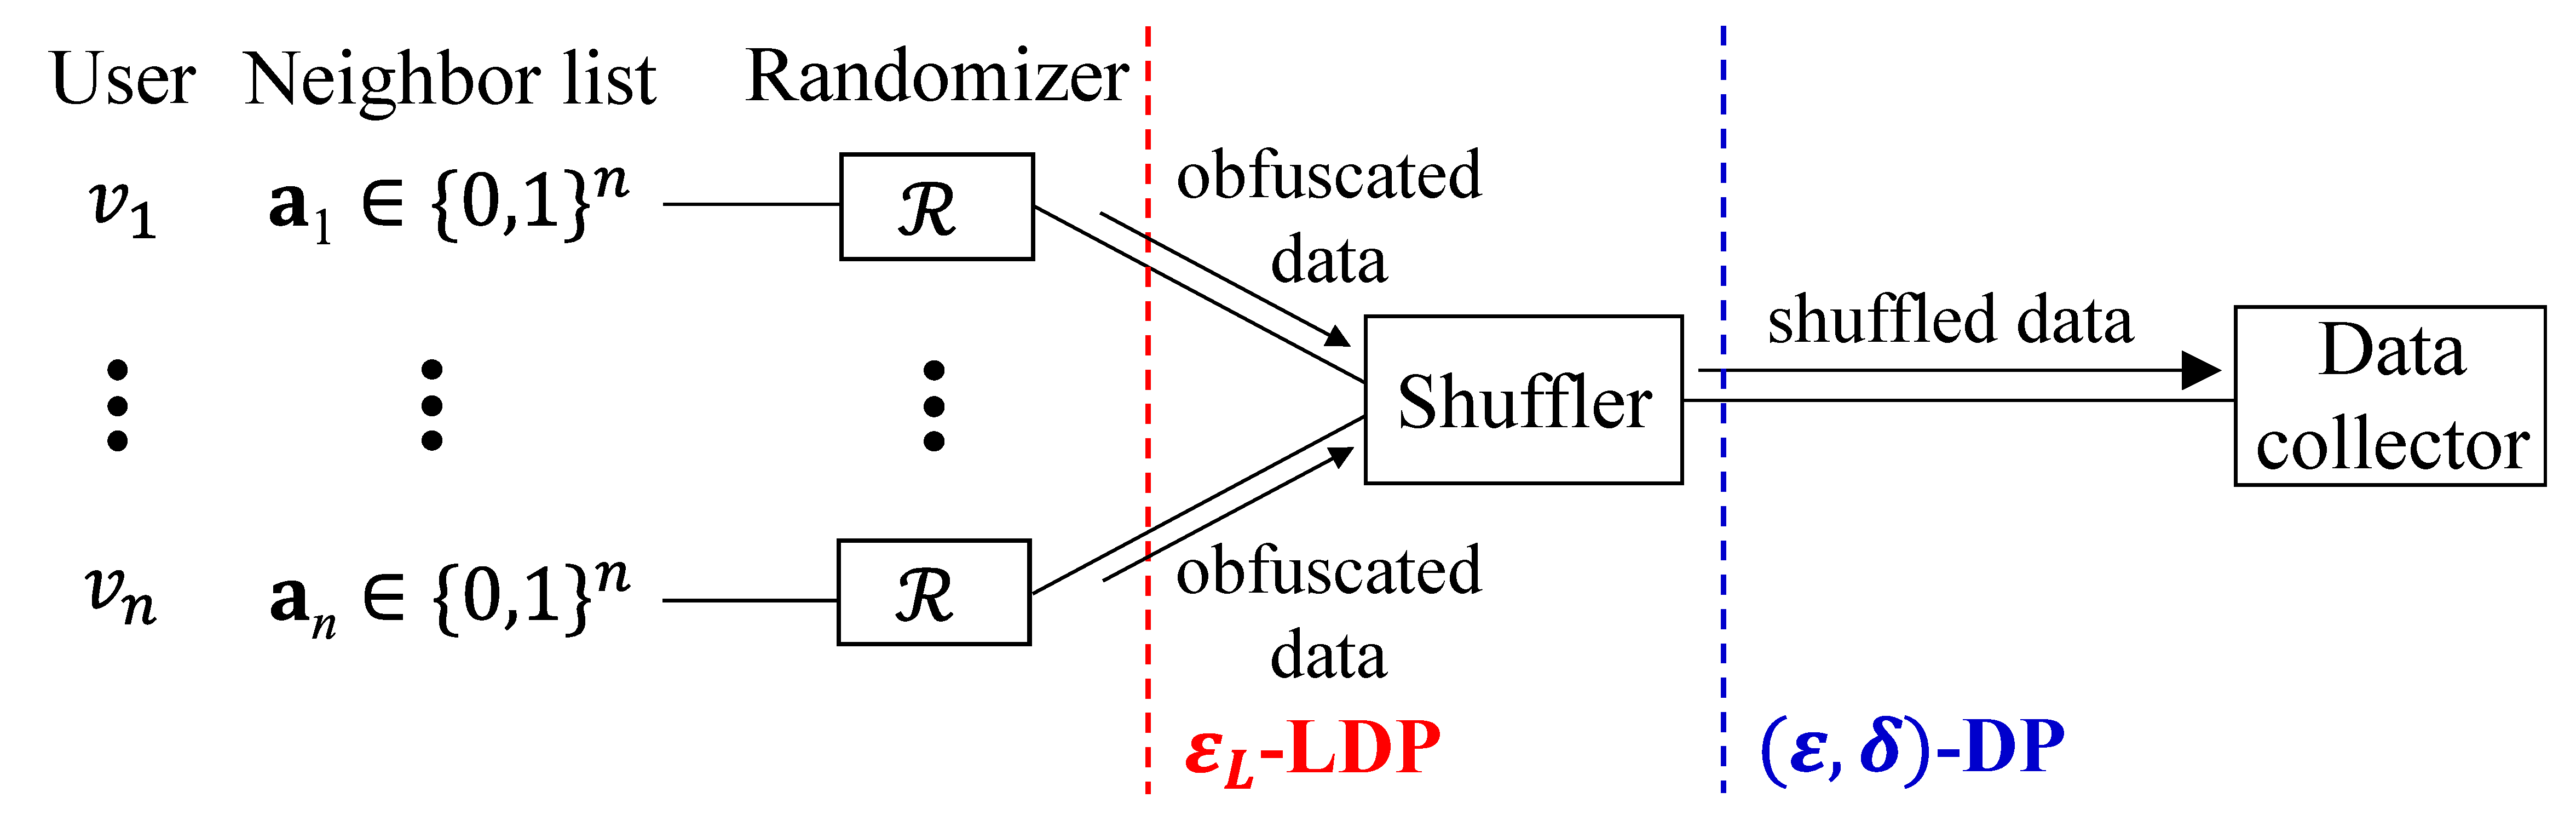
\includegraphics[width=0.99\linewidth]{fig/shuffle.pdf}
%   
%   \caption{Shuffle model. 
%   User $v_i$ obfuscates input data $x_i$ 
%   % calculated from her neighbor list $\bma_i$ 
%   and sends the obfuscated data $y_i$ to the shuffler. 
%   The shuffler sends shuffled data $y_{\pi(1)}, \ldots, y_{\pi(n)}$ to the data collector.
%   }
%   \label{chap3-fig:shuffle_model}
% \end{figure}
% Figure~\ref{chap3-fig:shuffle_model} shows the shuffle model assumed in this paper. 
Thanks to the shuffling, the shuffled data $y_{\pi(1)}, \ldots, y_{\pi(n)}$ available to the data collector provides $(\epsilon, \delta)$-DP, where $\epsilon \ll \epsilon_L$. 

Feldman \textit{et al.} \cite{Feldman_FOCS21} also propose an efficient method to numerically compute a tighter upper bound than the closed-form upper bound in Theorem~\ref{chap3-thm:shuffle}. 
We use both the closed-form and numerical upper bounds in our experiments. 
Specifically, we use the numerical upper bounds in Section~\ref{chap3-sec:experiments} and compare the numerical bound with the closed-form bound in 
\conference{the full version \cite{Imola_CCSFull22}}\arxiv{Appendix~\ref{chap3-sec:numerical_closed}}. 

Assume that $\epsilon$ and $\delta$ in (\ref{chap3-eq:shuffle_epsilon}) are constants. 
Then, by solving for $\epsilon_L$ and changing to big $O$ notation, we obtain  $\epsilon_L = \log(n) + O(1)$. 
This is consistent with the upper bound $\epsilon = O(e^{\epsilon_L / 2} / \sqrt{n})$ in \cite{Feldman_FOCS21}, from which we obtain $\epsilon_L = \log(n) + O(1)$. 
% By (\ref{chap3-eq:shuffle_epsilon}), when we treat $\epsilon$ and $\delta$ as constants, $\epsilon_L$ can be expressed as 
% $\epsilon_L = \log(n) + O(1)$. 
% Similarly, the privacy amplification bounds in \cite{Balle_CRYPTO19,Cheu_EUROCRYPT19} can also be expressed as $\epsilon_L = \Theta(\log(n))$. 
Similarly, the privacy amplification bound in \cite{Cheu_EUROCRYPT19} can also be expressed as $\epsilon_L = \log(n) + O(1)$. 
% This is smaller than other bounds, such as \cite{Balle_CRYPTO19,Erlingsson_SODA19}. 
We use the bound in \cite{Feldman_FOCS21} because it is the state-of-the-art, as described in Section~\ref{chap3-sec:related}. 
% -- it provides smaller $\epsilon$ than other bounds, such as \cite{Balle_CRYPTO19,Cheu_EUROCRYPT19,Erlingsson_SODA19}. 
%and is more general than the bound in \cite{Cheu_EUROCRYPT19} that is specific to binary RR. 
% The bound in \cite{Feldman_FOCS21} also outperforms the bound in \cite{Girgis_CCS21} when it is used without composition, which is the case with this work. 

% Note that the privacy amplification result in \cite{Feldman_FOCS21} assumes that the data elements are shuffled \textit{before} applying the local randomizers, i.e., shuffle-then-randomize. 
% However, 
% shuffling outputs of the same local randomizers (randomize-then-shuffle) 
% is equivalent to first shuffling input data and then applying the local randomizers (shuffle-then-randomize) as described in \cite{Erlingsson_SODA19}. 
% Thus, if all users adopt the same local randomizer, the result in \cite{Feldman_FOCS21} can be applied to the randomize-then-shuffle model, which gives Theorem~\ref{chap3-thm:shuffle}. 

\subsection{Utility Metrics}
\label{chap3-sub:utility}
% Following the existing work, 
We use 
the MSE (Mean Squared Error) 
% the expectation of the $l_2$ loss \cite{Kairouz_ICML16,Murakami_USENIX19,Wang_USENIX17} 
in our theoretical analysis and the relative error 
% \cite{Bindschaedler_SP16,Chen_CCS12,Xiao_SIGMOD11} 
in our experiments. 
The MSE is the expectation of the squared error 
% The $l_2$ loss is a squared error 
between a true value and its estimate. 
Let $f: \calG \rightarrow \nnints$ be a subgraph count function that can be instantiated by $f^\triangle$ or $f^\square$. 
Let $\hf: \calG \rightarrow \reals$ be the corresponding estimator. 
Let 
$\MSE: \reals \rightarrow \nnreals$ be the MSE function, which maps the estimate $\hf(G)$ to the MSE. 
% $l_2^2: \nnints \times \reals \rightarrow \nnreals$ be the expected $l_2$ loss function, which maps the true count $f(G)$ and the estimate $\hf(G)$ to the expected $l_2$ loss. 
Then the MSE can be expressed as $\MSE(\hf(G)) = \E[(f(G) - \hf(G))^2]$, 
% Then it can be expressed as $l_2^2(f(G), \hf(G)) = \E[(f(G) - \hf(G))^2]$, 
where the expectation is taken over the randomness in the estimator $\hf$. 
By the bias-variance decomposition \cite{mlpp}, 
the MSE can be expressed as a summation of the squared bias $(\E[\hf(G)] - f(G))^2$ and the variance $\V[\hf(G)] = \E[(\hf(G) - \E[\hf(G)])]^2$. 
Thus, for an unbiased estimator $\hf$ satisfying $\E[\hf(G)] = f(G)$, the MSE is equal to the variance, i.e., $\MSE(\hf(G)) = \V[\hf(G)]$. 

Although the MSE is suitable for theoretical analysis, it tends to be large when the number $n$ of users is large. 
This is because the true triangle and 4-cycle counts are very large when $n$ is large -- $f^\triangle(G) = O(n d_{max}^2)$ and $f^\square(G) = O(n d_{max}^3)$. 
Therefore, we use the relative error in our experiments. 
The relative error is an absolute error divided by the true value and is given by $\frac{|f^\triangle(G) - \hf^\triangle(G)|}{\min\{f^\triangle(G), \eta\}}$, where $\eta \in \nnreals$ is a small positive value. 
Following the convention \cite{Bindschaedler_SP16,Chen_CCS12,Xiao_SIGMOD11}, we set $\eta = \frac{n}{1000}$. 

When the relative error is well below $1$, the estimate is accurate. 
Note that the absolute error smaller than $1$ would be impossible under DP with meaningful $\epsilon$ (e.g., $\epsilon \leq 1$), as we consider counting queries. 
However, the relative error ($=$ absolute error / true count) much smaller than $1$ is possible under DP with meaningful $\epsilon$. 

\section{Shuffle Model for Graphs}
\label{sec:shuffle}
In this work, we apply the shuffle model to graph data to accurately estimate subgraph counts, such as triangles and 4-cycles. 
Section~\ref{sub:technical} explains our technical motivation. 
% the motivation of our approach. 
In particular, we explain why it is challenging to apply the shuffle model to graph data. 
Section~\ref{sub:wedge_shuffle} proposes a wedge shuffle technique to overcome the technical challenge. 

% \subsection{Technical Challenges}
\subsection{Our Technical Motivation}
\label{sub:technical}

\begin{figure}[t]
  \centering
  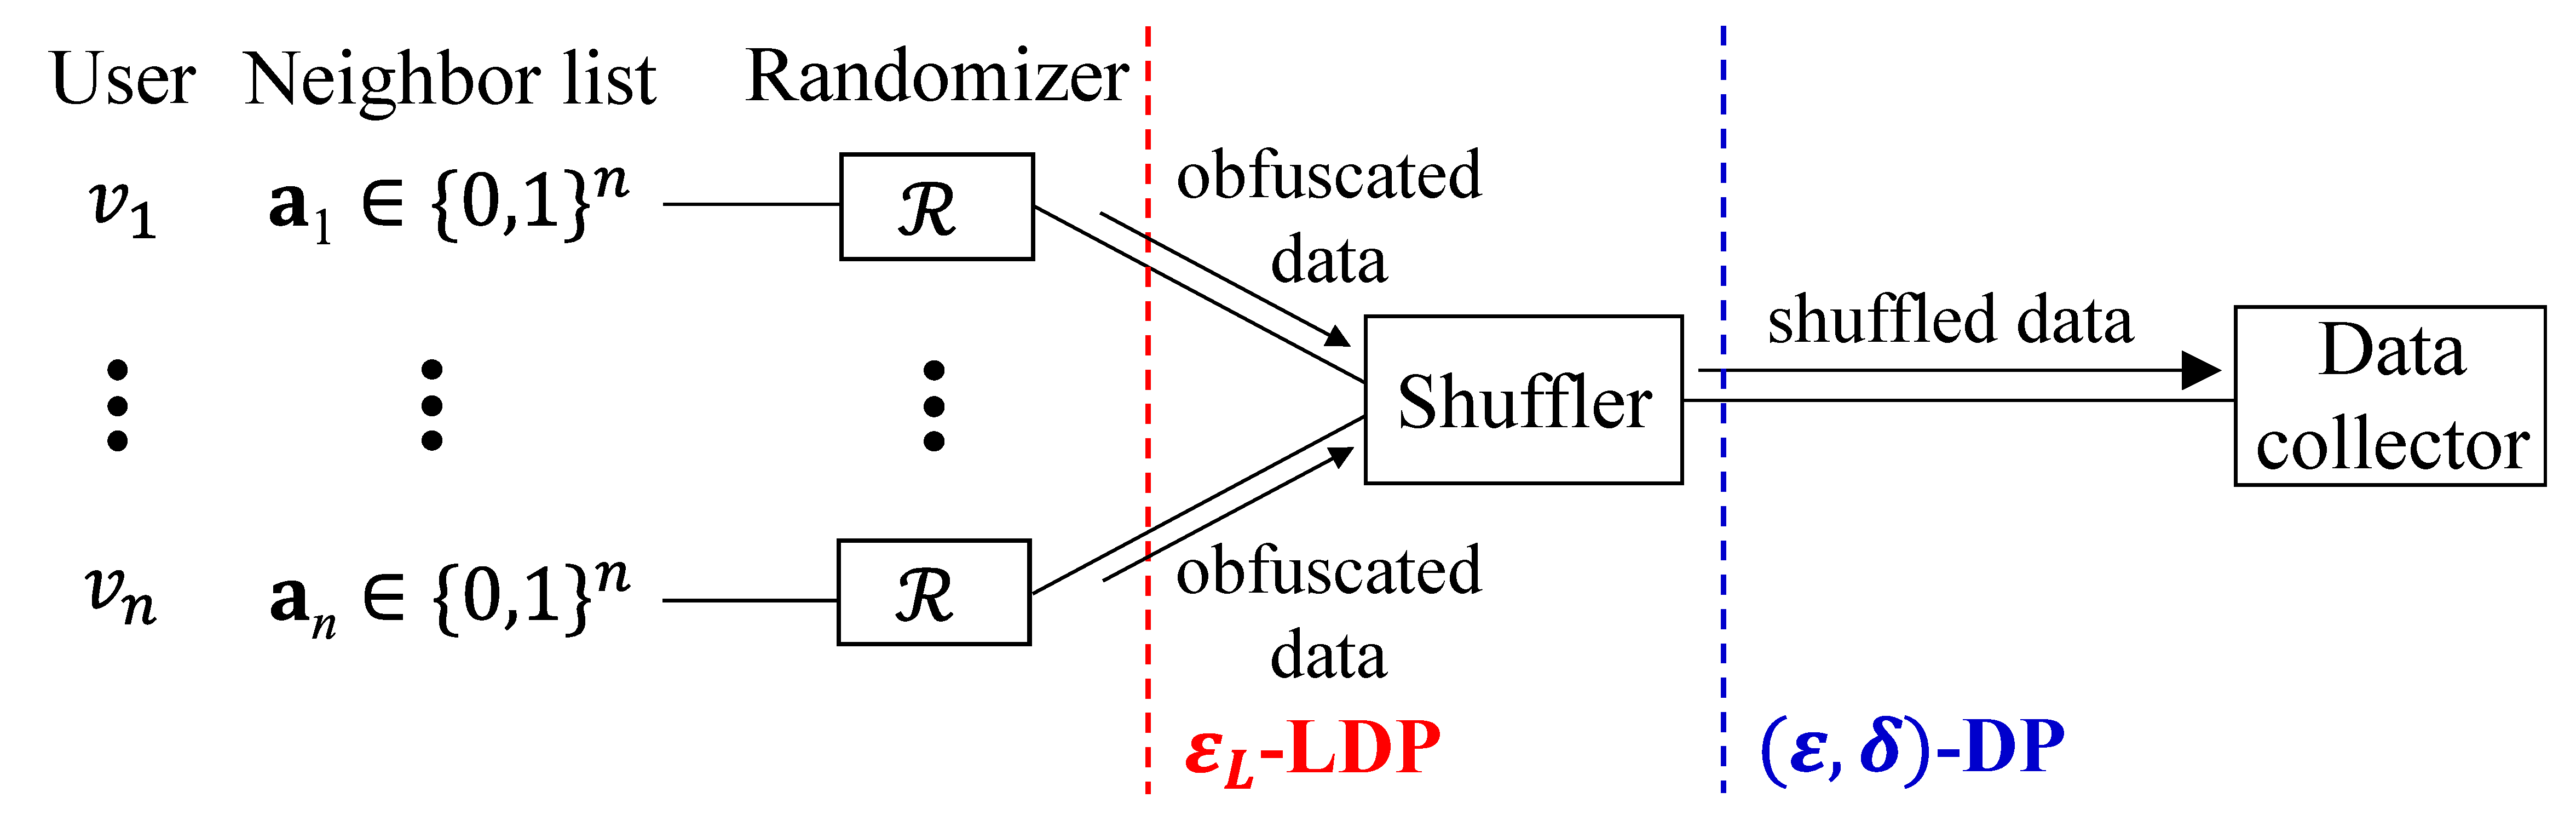
\includegraphics[width=0.99\linewidth]{fig/shuffle.pdf}
  \vspace{-2mm}
  \caption{Shuffle model for graphs. 
  %User $v_i$ calculates input data from her neighbor list $\bma_i$ and obfuscates the input data. 
  %The shuffler randomly shuffles the obfuscated data. 
  }
  \label{fig:shuffle_model}
\end{figure}

% the privacy-utility trade-off can be significantly improved 
% The privacy budget $\epsilon$ (hence the estimation error at the same value of $\epsilon$) can be dramatically reduced by introducing the shuffler. 
The shuffle model has been introduced to dramatically reduce the privacy budget $\epsilon$ (hence the estimation error at the same $\epsilon$) in tabular data \cite{Meehan_ICLR22,Wang_PVLDB20} or 
% image data 
gradients 
\cite{Girgis_AISTATS21,Liu_AAAI21}. 
However, it is very challenging to apply the shuffle model to graph data, 
% analysis, 
as explained below. 

Figure~\ref{fig:shuffle_model} shows the shuffle model for graph data, where each user $v_i$ has her neighbor list $\bma_i \in \{0,1\}^n$. 
% The main reason for this 
The main challenge here 
% in the graph shuffle model 
is that 
% because 
the shuffle model uses a \textit{standard} definition of LDP for the local randomizer and that a neighbor list is \textit{high-dimensional data}, i.e., $n$-dim binary string. 
Specifically, LDP in Definition~\ref{def:LDP} requires any pair of inputs $x$ and $x'$ to be indistinguishable; i.e., 
the inequality (\ref{eq:LDP}) must hold for all pairs of possible inputs. 
Thus, if we use the entire neighbor list 
% (i.e., $n$-dim binary string) 
as input data (i.e., $\bma_i = x_i$ in Theorem~\ref{thm:shuffle}), 
% the standard LDP definition destroys 
either privacy or utility is destroyed for large $n$. 

To illustrate this, consider the following example. 
Assume that $n=10^5$ and $\delta=10^{-8}$. 
Each user $v_i$ applies 
% Warner's RR 
$\epsilon_0$-RR 
with $\epsilon_0=1$ to each bit of her neighbor list $\bma_i$. 
This mechanism is called the randomized neighbor list \cite{Qin_CCS17} and provides $\epsilon_0$-edge LDP. 
% which considers two neighbor lists that differ in one bit. 
However, the privacy budget $\epsilon_L$ in the standard LDP (Definition~\ref{def:LDP}) 
is extremely large -- by group privacy \cite{DP}, $\epsilon_L = n \epsilon_0 = 10^5$. 
Because 
$\epsilon_L$ 
% $n\epsilon$ 
is much larger than $\log (\frac{n}{16 \log (2/\delta)}) = 8.09$, we cannot use the privacy amplification result in Theorem~\ref{thm:shuffle}. 
This is evident from the fact that the shuffled data $y_{\pi(1)}, \ldots, y_{\pi(n)}$ are easily re-identified when $n$ is large. 
If we use 
% Warner's RR 
$\epsilon_0$-RR 
with $\epsilon_0 = \frac{1}{n}$, we can use the amplification result (as $\epsilon_L = n \epsilon_0 = 1$). 
However, it makes obfuscated data almost a random string and destroys the utility because $\epsilon_0$ is too small. 

In this work, we address this issue by introducing a basic technique, which we call \textit{wedge shuffling}. 

\subsection{Our Approach: Wedge Shuffling}
\label{sub:wedge_shuffle}

% To accurately count subgraphs such as triangles and 4-cycles, we propose a basic technique, which we call \textit{wedge shuffling}. 

% \smallskip
% \noindent{\textbf{Overview.}}~~
Figure ~\ref{fig:wedge_shuffle} shows the overview of our wedge shuffle technique. 
% First, we propose a basic technique, which we call wedge shuffling, to enable privacy amplification of graph data by shuffling. 
This technique calculates the number of wedges (2-hop paths) between 
% a specific user-pair $(v_i, v_j)$. 
a specific pair of users $v_i$ and $v_j$. 
%from user $v_i$ to $v_j$. 

Algorithm~\ref{alg:WShuffle} shows our wedge shuffle algorithm, which we call \AlgWS{}. 
% Specifically, 
% we consider the problem of counting triangles including a specific user-pair $(v_i, v_j)$ 
% and propose a wedge shuffle algorithm to accurately count them. 
Given users $v_i$ and $v_j$, 
% our wedge shuffle algorithm calculates 
each of the remaining users $v_k$ ($k \ne i, j$) 
% \in [n]\setminus\{i,j\}$) 
calculates a \textit{wedge indicator} $w_{i-k-j} = a_{k,i} a_{k,j}$, 
%\in \{0,1\}$, 
which 
takes $1$ if 
%and only if 
a wedge $v_i$-$v_k$-$v_j$ exists and $0$ otherwise (line 2). 
Then, $v_k$ obfuscates $w_{i-k-j}$ using $\epsilon_L$-RR and sends it to the shuffler (line 3). 
The shuffler randomly shuffles the noisy wedges using a random permutation $\pi$ over 
% $[n-2]$ 
% $[n]\setminus\{i,j\}$ 
$I_{-(i,j)}$ ($=[n]\setminus\{i,j\}$) 
to provide $(\epsilon, \delta)$-DP with $\epsilon \ll \epsilon_L$ (line 5). 
Finally, the shuffler sends the shuffled wedges to the data collector (line 6). 
The only information available to the data collector is  the number of wedges from $v_i$ to $v_j$, i.e., 
% the number of 
common friends of $v_i$ and $v_j$. 

Our wedge shuffling has two main features. 
First, 
% Because 
the wedge indicator $w_{i-k-j}$ is \textit{one-dimensional binary data}. 
Therefore, it can be sent with small noise and small $\epsilon$, unlike the $n$-dimensional neighbor list. 
For example, when $n=10^5$, $\delta=10^{-8}$, and $\epsilon=1$, the value of $\epsilon_L$ in (\ref{eq:shuffle_epsilon_f}) and (\ref{eq:shuffle_epsilon}) is $\epsilon_L = 5.44$. In this case, $\epsilon_L$-RR rarely flips $w_{i-k-j}$ -- the flip probability is $0.0043$. 
In other words, the shuffled wedges are almost free of noise. 

\begin{figure}[t]
  \centering
  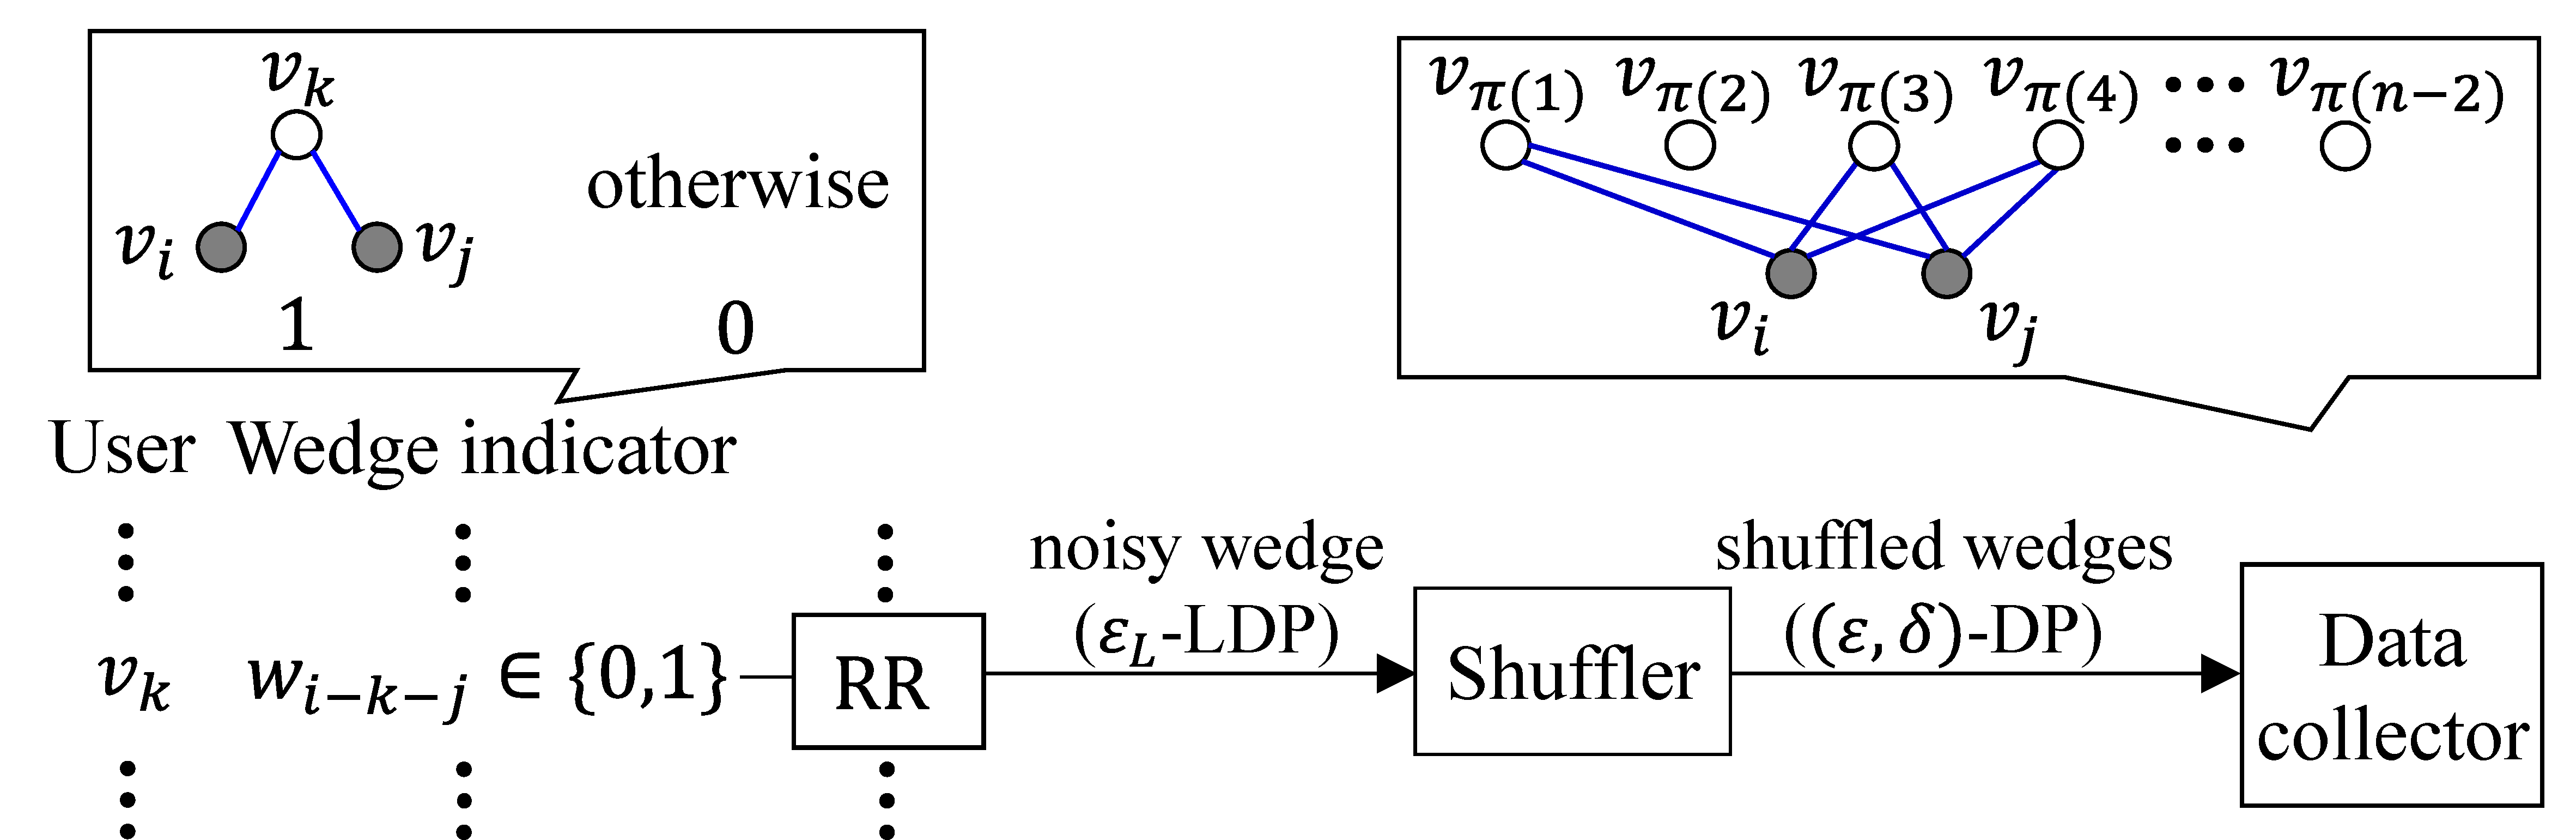
\includegraphics[width=0.99\linewidth]{fig/wedge_shuffle.pdf}
  \vspace{-2mm}
  \caption{Overview of wedge shuffling with inputs $v_i$ and $v_j$. 
  %(marked with gray).
  }
  \label{fig:wedge_shuffle}
\end{figure}

\setlength{\algomargin}{5mm}
\begin{algorithm}[t]
  \SetAlgoLined
  \KwData{Adjacency matrix $\bmA \in \{0,1\}^{n \times n}$, $\epsilon_L \in \nnreals$, user-pair $(v_i,v_j)$.}
  \KwResult{Shuffled wedges $\{y_{\pi(k)} | k \in I_{-(i,j)}\}$.}
%   \tcc{Set-up}
%   $I_{-(i,j)} \leftarrow [n]\setminus\{i,j\}$\;
%   $\epsilon_L \leftarrow \texttt{LocalPrivacyBudget}(n,\epsilon,\delta)$\;
%   \tcc{Users}
  \ForEach{$k \in I_{-(i,j)}$}{
    [$v_k$] $w_{i-k-j} \leftarrow a_{k,i} a_{k,j}$\;
    [$v_k$] $y_k \leftarrow \calR_{\epsilon_L}^W(x)(w_{i-k-j})$; Send $y_k$ to the shuffler\;
  }
%   \tcc{Shuffler}
  [s] Sample a random permutation $\pi$ over $I_{-(i,j)}$\;
  [s] Send $\{y_{\pi(k)} | k \in I_{-(i,j)}\}$ to the data collector\;
%   \tcc{Data collector}
  [d] \KwRet{$\{y_{\pi(k)} | k \in I_{-(i,j)}\}$}
  \caption{Our wedge shuffle algorithm \AlgWS{}. 
  [$v_k$], [s], and [d] represent that the process is run by user $v_i$, the shuffler, and the data collector, respectively. 
  }\label{alg:WShuffle}
\end{algorithm}

Second, the wedge is the main component of many subgraphs such as triangles, 
$k$-triangles \cite{Karwa_PVLDB11}, 
3-hop paths \cite{Sun_CCS19}, 
and 4-cycles. 
For example, a triangle consists of one wedge and one edge, e.g., $v_i-v_{\pi(3)}-v_j$ and $(v_i, v_j)$ in Figure ~\ref{fig:wedge_shuffle}. 
More generally, a $k$-triangle consists of $k$ triangles sharing one edge. 
Thus, it can be decomposed into $k$ wedges and one edge. 
% Similarly, a 
A 3-hop path consists of one wedge and one edge. 
A 4-cycle consists of two wedges, e.g., $v_i-v_{\pi(1)}-v_j$ and $v_i-v_{\pi(3)}-v_j$ in Figure ~\ref{fig:wedge_shuffle}. 
Because the shuffled wedges have little noise, we can accurately count these subgraphs based on wedge shuffling, compared to local algorithms in which all edges are noisy. 
% The other components can be sent from users to the data collector directly (or through the shuffler without shuffling) after adding LDP noise, e.g., by Warner's RR. 
% For example, if the data collector has a noisy edge between $v_i$ and $v_j$, it can count triangles including $(v_i, v_j)$. 
% Similarly, the data collector can count $k$-triangles that consist of $k$ triangles sharing $(v_i, v_j)$. 
% % Because the shuffled wedges have little noise, our wedge shuffling can significantly reduce the DP noise when compared to local algorithms. 
% Moreover, the data collector can count 4-cycles including $v_i$ and $v_j$ (e.g., $v_i-v_{\pi(1)}-v_j-v_{\pi(3)}-v_i$ in Figure ~\ref{fig:wedge_shuffle}) based only on the shuffled wedges. 
% Because the shuffled wedges have little noise, we can accurately count these subgraphs by sampling user-pairs and shuffling wedges. 

In this work, we focus on triangles and 4-cycles and 
present algorithms with upper bounds on the estimation error based on our wedge shuffle technique. 
% use our wedge shuffle technique for accurately counting them. 

% \smallskip
% \noindent{\textbf{Algorithm.}}~~Algorithm~\ref{alg:WShuffle} shows 

% \subsection{Algorithm}
% \label{sub:4cycle_algorithm}
% TBD

% \subsection{Theoretical Analysis}
% \label{sub:4cycle_theoretical}
% TBD

%!TEX root=main.tex
% \section{Differentially Private Triangle Counting under the Shuffle Model}
% \section{Triangle Counting}
\section{Triangle Counting Based on Wedge Shuffling}
\label{sec:triangle}
% The existing one-round local triangle algorithms \cite{Imola_USENIX21,Imola_USENIX22,Ye_ICDE20,Ye_TKDE21} suffer from an extremely large estimation error; e.g., when $\epsilon=1$ in edge DP, the relative error is much larger than $1$ in our experiments.
% To address this issue, we propose a differentially private one-round triangle counting algorithm based on wedge shuffling.
Based on our wedge shuffle technique, we first propose a
% differentially private
one-round triangle counting algorithm.
% in the shuffle model.
%
% Section~\ref{sub:challenges} explains technical challenges in our work.
% In particular, we explain why it is challenging to apply the shuffle model to graph data.
Section~\ref{sub:triangle_overview} describes the overview of our algorithms.
Section~\ref{sub:wedge} proposes an algorithm for counting triangles involving a specific user-pair
% proposes a wedge shuffle technique
as a building block of our triangle counting algorithm.
Section~\ref{sub:triangle} proposes
our triangle counting algorithm.
%an algorithm for counting triangles in the entire graph.
% a one-round triangle counting algorithm based on the wedge shuffling.
Section~\ref{sub:var_red} proposes a technique to significantly reduce the variance in our triangle counting algorithm. 
% by ignoring sparse user-pairs.
Section~\ref{sub:summary} summarizes the performance guarantees of our triangle algorithms. 
% The proofs of all statements in this section are given in Appendix~\ref{sec:triangle_proof}.

% \subsection{Technical Challenges}
% \label{sub:challenges}
% The limitation of the one-round local triangle algorithms is an extremely large estimation error.
% This limitation comes from the fact that all three edges are noisy in any noisy edge the data collector can see, as described in Section~\ref{sec:intro}.

% \subsection{Algorithm Overview}
\subsection{Overview}
\label{sub:triangle_overview}
Our wedge shuffle technique tells the data collector the number of common friends of $v_i$ and $v_j$.
However, this information is not sufficient to count triangles in the entire graph.
% the data collector still cannot count triangles, because she does not know whether $v_i$ and $v_j$ are friends.
% To accurately count triangles based on wedge shuffling,
% under the shuffle model,
Therefore, we introduce
% four
three additional techniques:
% strategies:
% \textit{(i) shuffling wedges},
\textit{(i) sending local edges},
% \textit{wedge shuffling},
% \textit{edge sampling without replacement}.
% \textit{sampling independent edges},
% \textit{sampling independent pairs of nodes}.
\textit{(ii) sampling disjoint user-pairs},
% \textit{independent edge sampling},
and
\textit{(iii) variance reduction by ignoring sparse user-pairs}.
% Our wedge shuffle algorithm uses the first and second strategies, whereas our one-round triangle counting algorithm uses the third and fourth strategies.
% Figures~\ref{fig:local_edges} and \ref{fig:triangle_count} show the overview of our wedge shuffle and triangle counting algorithms, respectively.
% the first two strategies and the third strategy, respectively.
Below, we briefly explain each technique.

\begin{figure}[t]
  \centering
  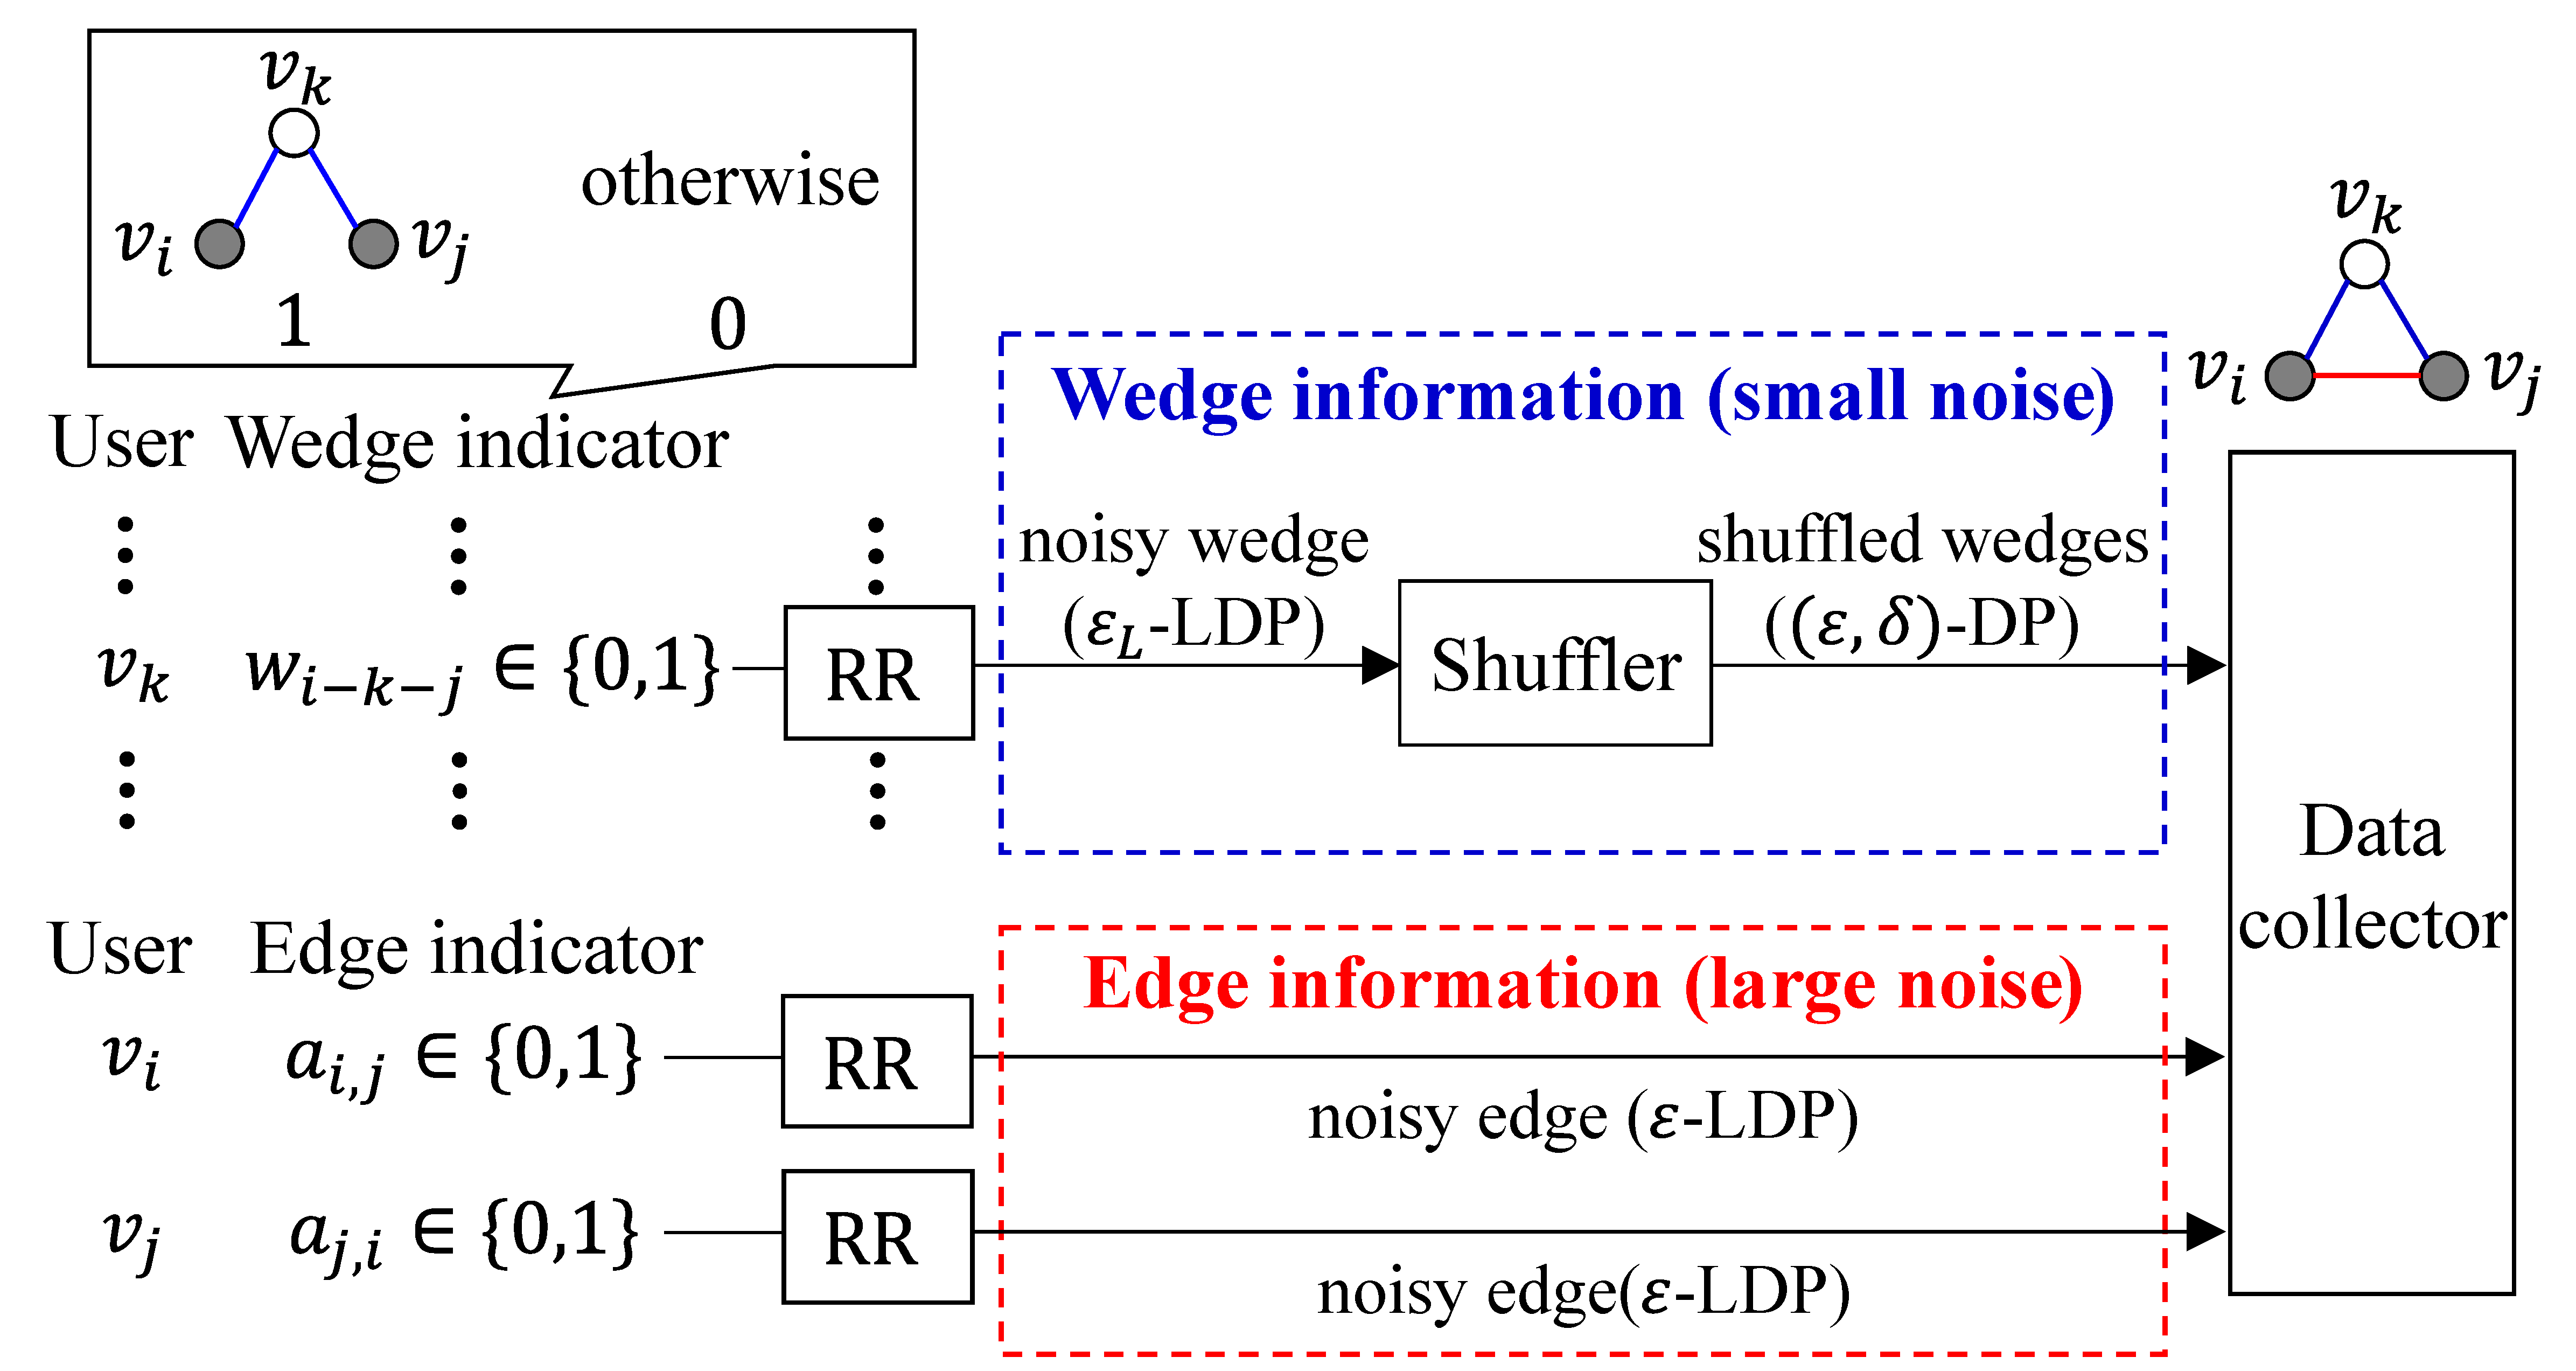
\includegraphics[width=0.99\linewidth]{fig/local_edges.pdf}
  \vspace{-2mm}
  \caption{Overview of our \AlgWSLE{} (Wedge Shuffling with Local Edges) algorithm with inputs $v_i$ and $v_j$.
  %our wedge shuffle algorithm with inputs $v_i$ and $v_j$.
  %(marked with gray).
  }
  \label{fig:local_edges}
% \end{figure}
\vspace{2mm}
% \begin{figure}[t]
  \centering
  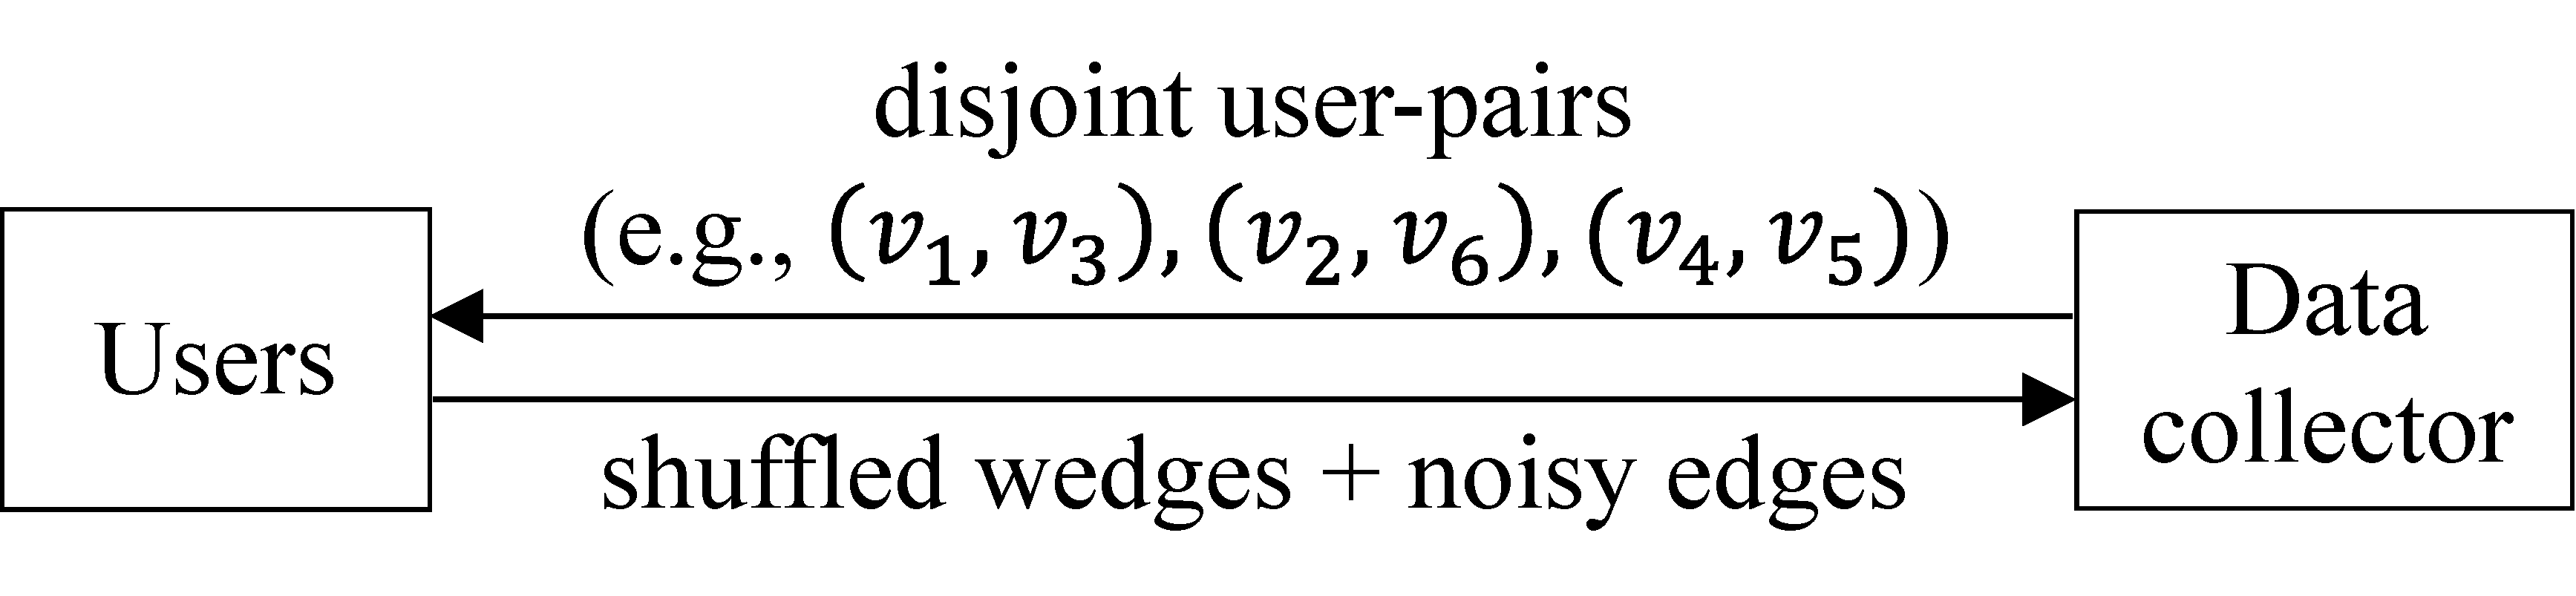
\includegraphics[width=0.7\linewidth]{fig/sampling_pairs2.pdf}
  \vspace{-2mm}
  \caption{Overview of our triangle counting algorithm.
  We use our
  %wedge shuffle
  \AlgWSLE{}
  algorithm with each user-pair.
  %Independent pairs of nodes do share common nodes, e.g., $(v_1, v_3)$, $(v_2, v_6)$, $(v_4, v_5)$.
  }
  \label{fig:triangle_count}
\end{figure}

\smallskip
\noindent{\textbf{Sending Local Edges.}}~~First, we consider the problem of counting triangles involving a specific user-pair $(v_i, v_j)$ and propose an algorithm to send
% The shuffled wedge indicators tell us the number of common friends of $v_i$ and $v_j$.
% However, the data collector still cannot count triangles, because she does not know whether $v_i$ and $v_j$ are friends.
% Thus, our wedge shuffle algorithm sends
\textit{local edges} between $v_i$ and $v_j$, along with shuffled wedges, to the data collector.
We call this the \AlgWSLE{} (Wedge Shuffling with Local Edges) algorithm.
%algorithm \AlgWSLE{} (Wedge Shuffle Edge Local).
% the \textit{wedge shuffling with local edges} algorithm and abbreviate it to \AlgWSLE{}.

Figure~\ref{fig:local_edges} shows the overview of \AlgWSLE{}.
In this algorithm, users $v_i$ and $v_j$ obfuscate edge indicators $a_{i,j}$ and $a_{j,i}$, respectively, using $\epsilon$-RR and send them to the data collector directly (or through the shuffler without shuffling).
%\footnote{It is also possible to send the noisy edge indicators from users $v_i$ and $v_j$ to the data collector through the shuffler. In this case, the shuffler does not shuffle these data.}.
Then, the data collector calculates an unbiased estimate of the triangle count
% from the noisy data.
from the shuffled wedges and the noisy edges.
Because $\epsilon$ is small, a large amount of noise is added to the edge indicators.
However, \textit{only one edge} is noisy (the other two have little noise) in any triangle the data collector sees.
This brings us an advantage over the one-round local algorithms in which all three edges are noisy.

\smallskip
\noindent{\textbf{Sampling Disjoint User-Pairs.}}~~Next, we consider the problem of counting triangles in the entire graph $G$.
A naive solution to this problem is to use our
%wedge shuffling
\AlgWSLE{} algorithm
with all $\binom{n}{2}$ user-pairs as input.
However, it results in very large $\epsilon$ and $\delta$ because it uses each element of the adjacency matrix $\bmA$ many times.
To address this issue,
% To accurately count them under DP,
we propose a triangle counting algorithm that samples
% independent edges (a.k.a. matching), which have no nodes in common.
disjoint user-pairs, ensuring that no user falls in two pairs. 
% which share no common users.
% and then uses the wedge shuffling algorithm for each sampled edge.

Figure~\ref{fig:triangle_count} shows the overview of our triangle algorithm.
The data collector sends the sampled user-pairs to users.
Then, users apply
%our wedge shuffling algorithm
\AlgWSLE{}
with each user-pair
% as input
and send the results to the data collector.
Finally, the data collector calculates an unbiased estimate of the triangle count from the results.
% This can be viewed as edge sampling \cite{Bera_KDD20,Eden_FOCS15,Wu_TKDE16} in triangle counting.
% Edge sampling is known as an efficient sampling method that outperforms other sampling methods such as node sampling and triangle sampling \cite{Wu_TKDE16}.
% Our triangle counting algorithm is also efficient and
% In fact,
Because our triangle algorithm uses each element of
% the adjacency matrix
$\bmA$ \textit{at most once}, it provides $(\epsilon,\delta)$-element DP hence $(2\epsilon,2\delta)$-edge DP.
In addition, our triangle algorithm reduces the time complexity from $O(n^3)$ to $O(n^2)$ by sampling user-pairs rather than using all user-pairs.
% In addition, our wedge shuffle algorithm with a user-pair $(v_i,v_j)$ provides $(\epsilon,\delta)$-DP for each row in the $i$-th and $j$-th columns of the adjacency matrix $\bmA$, and our triangle algorithm samples independent user-pairs.
% Thus, our algorithm provides $(\epsilon,\delta)$-element DP hence $(2\epsilon,2\delta)$-edge DP.

We prove that the MSE of our triangle counting algorithm is
% $O(n^3 d_{max}^2)$.
$O(n^3)$ when we ignore the factor of $d_{max}$.
% when we regard $\epsilon$ and $\delta$ as constants.
When we do not shuffle wedges, the
% expected
MSE is
% $O(n^5)$.
$O(n^4)$.
% This is much smaller than the existing one-round local algorithm with the same time complexity, whose $l_2$ loss is $O(n^5)$, as shown in Section~\ref{sub:upper}.
In addition, the MSE of the existing one-round local algorithm \cite{Imola_USENIX22} with the same time complexity is $O(n^6)$, as proved in
\conference{the full version \cite{Imola_CCSFull22}}\arxiv{
Appendix~\ref{sec:upper}}.
% Section~\ref{sub:upper}.
% Thus, our algorithm has a much smaller estimation error than the local algorithm.
Thus, our
% wedge shuffling
algorithm
provides a dramatic improvement over the local algorithms.

\smallskip
\noindent{\textbf{Variance Reduction.}}~~Although our
% wedge shuffling
algorithm
dramatically
% reduces
improves
the MSE, the factor of $n^3$ may still be large.
Therefore, we propose a variance reduction technique that ignores sparse user-pairs, where either of the two users has a very small degree.
Our basic idea is that the number of triangles involving such a user-pair is very small
% such user-pairs have a very small number of triangles
and can be approximated by $0$.
By ignoring the sparse user-pairs, we can significantly reduce the variance at the cost of introducing a small bias.
We prove that our variance reduction technique reduces the MSE from $O(n^3)$ to $O(n^\gamma)$ where $\gamma\in[2,3)$ and makes one-round triangle counting more accurate.
%accurate one-round triangle counting possible.
% This enables us to accurately count triangles within one round.


% \subsection{Triangle Counting Including a Specific User-Pair}
% \label{sub:triangle_edge}
% \subsection{Wedge Shuffling with Local Edges}
\subsection{WSLE (Wedge Shuffling with Local Edges)}
% \subsection{Sending Local Edges}
\label{sub:wedge}
% Each user $v_k$ ($k \ne i, j$) calculates wedge information $w_{i-k-j} \in \{0,1\}$ that takes $1$ if there is a two-hop path $v_i-v_k-v_j$ and 0 otherwise.
% Then $v_k$ obfuscates $w_{i-k-j}$ using $\epsilon_L$-RR and sends the noisy wedge to the shuffler.
% The shuffler randomly shuffles the noisy wedges to provide $(\epsilon, \delta)$-DP with $\epsilon \ll \epsilon_L$ and sends them to the data collector.
% In addition, users $v_i$ and $v_j$ obfuscate edge information $a_{i,j}$ and $a_{j,i}$, respectively, using $\epsilon$-RR and directly send them to the data collector.

% \smallskip
\noindent{\textbf{Algorithm.}}~~We first
%Consider the problem of counting triangles including a specific user-pair $(v_i,v_j)$.
% To solve this problem, we
propose
% a wedge shuffle algorithm,
the \AlgWSLE{} algorithm
as a building block of our triangle counting algorithm.
\AlgWSLE{} counts
% which estimates the number of
triangles involving a specific user-pair $(v_i,v_j)$.
% We denote this algorithm by \AlgWSLE{}.

Algorithm~\ref{alg:WSLE} shows \AlgWSLE{}.
% This algorithm estimates the number of triangles including a specific user-pair $(v_i,v_j)$.
Let $f_{i,j}^\triangle: \calG \rightarrow \nnints$ be a function that takes $G \in \calG$ as input and outputs the number $f_{i,j}^\triangle(G)$ of triangles involving $(v_i,v_j)$ in $G$.
Let $\hf_{i,j}^\triangle(G) \in \reals$ be an estimate of $f_{i,j}^\triangle(G)$.
% Let $I_{-(i,j)}$ be the set of indices of users other than $v_i$ and $v_j$, i.e., $I_{-(i,j)} = [n]\setminus\{i,j\}$.

\setlength{\algomargin}{5mm}
\begin{algorithm}[t]
  \SetAlgoLined
  \KwData{Adjacency matrix $\bmA \in \{0,1\}^{n \times n}$,
    %Neighbor lists $\bma_1, \ldots, \bma_n \in \{0,1\}^n$,
    %$\epsilon_L \in \nnreals$, $\delta \in [0,1]$, $\epsilon = f(n-2, \epsilon_L, \delta)$,
    $\epsilon \in \nnreals$, $\delta \in [0,1]$,
    user-pair $(v_i,v_j)$.
  }
  \KwResult{Estimate $\hf_{i,j}^\triangle(G)$ of the number $f_{i,j}^\triangle(G)$ of triangles involving $(v_i,v_j)$.}
  %of the count of triangles including $(v_i,v_j)$.}
%   $I_{-(i,j)} \leftarrow [n]\setminus\{i,j\}$\;
%   $q_L \leftarrow \frac{1}{e^{\epsilon_L}+1}$; $q \leftarrow
  %   \frac{1}{e^\epsilon+1}$\;
  $\epsilon_L \leftarrow \texttt{LocalPrivacyBudget}(n,\epsilon,\delta)$\;
%   $\{y_{\pi(k)} | k \in I_{-(i,j)}\} \leftarrow$ \AlgWS{}$(\bmA, \epsilon, \delta, (v_{\sigma(i)}, v_{\sigma(i+1)}))$\;
  \tcc{Wedge shuffling}
  $\{y_{\pi(k)} | k \in I_{-(i,j)}\} \leftarrow$ \AlgWS{}$(\bmA, \epsilon_L, (v_i, v_j))$\;
  \tcc{Send local edges}
%   \For{$i=1$ \KwTo $n$}{
%   \ForEach{$k \in I_{-(i,j)}$}{
%     [$v_k$] $w_{i-k-j} \leftarrow a_{k,i} a_{k,j}$\;
%     [$v_k$] $y_k \leftarrow \calR_{\epsilon_L}^W(x)(w_{i-k-j})$\;
%     [$v_k$] Send $y_k$ to the shuffler\;
%   }
  [$v_i$] $z_i \leftarrow \calR_{\epsilon}^W(x)(a_{i,j})$; Send $z_i$ to the data collector\;
  [$v_j$] $z_j \leftarrow \calR_{\epsilon}^W(x)(a_{j,i})$; Send $z_j$ to the data collector\;
%   \tcc{Shuffler}
%   [s] Sample a random permutation $\pi$ over $I_{-(i,j)}$\;
%   [s] Send $\{y_{\pi(k)} | k \in I_{-(i,j)}\}$ to the data collector\;
  \tcc{Calculate an unbiased estimate}
  [d] $q_L \leftarrow \frac{1}{e^{\epsilon_L}+1}$; $q \leftarrow
  \frac{1}{e^\epsilon+1}$\;
  [d] $\hf_{i,j}^\triangle(G) \leftarrow \frac{(z_i+z_j-2q)\sum_{k \in
  I_{-(i,j)}} (y_{k} - q_L)}{2(1-2q)(1-2q_L)}$\;
  [d] \KwRet{$\hf_{i,j}^\triangle(G)$}
  \caption{\AlgWSLE{}
  %Our wedge shuffle algorithm
  (Wedge Shuffling with Local Edges).
  \AlgWS{} is shown in Algorithm~\ref{alg:WShuffle}.
  %[$v_i$], [s], and [d] represent that the process is run by user $v_i$, the shuffler, and the data collector, respectively.
  % Lines 1 and 2 are run by all parties.
  }\label{alg:WSLE}
\end{algorithm}

% Given $\epsilon$ and $\delta$,
We first call the function \texttt{LocalPrivacyBudget}, which calculates a local privacy budget $\epsilon_L$ from $n$, $\epsilon$, and $\delta$ (line 1).
Specifically, this function calculates $\epsilon_L$
such that $\epsilon$ is a closed-form upper bound (i.e., $\epsilon = f(n-2, \epsilon_L, \delta)$ in (\ref{eq:shuffle_epsilon_f})) or numerical upper bound in the shuffle model with $n-2$ users.
% \cite{Feldman_FOCS21}.
Given $\epsilon_L$, we can easily calculate the closed-form or numerical upper bound $\epsilon$ by (\ref{eq:shuffle_epsilon}) and the open source code in \cite{Feldman_FOCS21}\footnote{\url{https://github.com/apple/ml-shuffling-amplification}.}, respectively.
Thus, we can also easily calculate $\epsilon_L$ from $\epsilon$ by calculating a lookup table for pairs $(\epsilon, \epsilon_L)$ in advance.

Then, we run our wedge shuffle algorithm \AlgWS{} in Algorithm~\ref{alg:WShuffle} (line 2); i.e., each user $v_k \in I_{-(i,j)}$ sends her obfuscated wedge indicator
% obfuscates $w_{i-k-j}$ using $\epsilon_L$-RR $\calR_{\epsilon_L}^W$ and sends the result
$y_k = \calR_{\epsilon_L}^W(w_{i-k-j})$ to the shuffler, and the shuffler sends
shuffled wedge indicators $\{y_{\pi(k)} | k \in I_{-(i,j)}\}$ to the data collector.
%calculates a wedge indicator $w_{i-k-j} \in \{0,1\}$ from her neighbor list $\bma_k$ as follows: $w_{i-k-j} = a_{k,i} a_{k,j}$.
%User $v_k$
% (lines 4-6).
Meanwhile, user $v_i$ obfuscates her edge indicator $a_{i,j}$ using $\epsilon$-RR $\calR_{\epsilon}^W$ and sends the result $z_i = \calR_{\epsilon}^W(a_{i,j})$ to the data collector
% \footnotemark[1]
(line 3).
Similarly, $v_j$ sends $z_j = \calR_{\epsilon}^W(a_{j,i})$ to the data collector (line 4).

% The shuffler samples a uniform random permutation $\pi$ over $I_{-(i,j)}$ and shuffles the wedge indicators based on $\pi$.
% Then, the shuffler sends the shuffled wedge indicators $\{y_{\pi(k)} | k \in I_{-(i,j)}\}$ to the data collector (lines 12-13).

% After receiving $\{y_{\pi(k)} | k \in I_{-(i,j)}\}$, $z_i$, and $z_j$,
Finally, the data collector estimates $f_{i,j}^\triangle(G)$ from $\{y_{\pi(k)} | k \in I_{-(i,j)}\}$, $z_i$, and $z_j$.
% Specifically, let $\hf_{i,j}^\triangle(G) \in \reals$ be an estimate of $f_{i,j}^\triangle(G)$.
Specifically, the data collector calculates the estimate $\hf_{i,j}^\triangle(G)$ as follows:
\begin{align}
    \textstyle{\hf_{i,j}^\triangle(G) = \frac{(z_i+z_j-2q)\sum_{k \in I_{-(i,j)}} (y_{k} -
    q_L)}{2(1-2q)(1-2q_L)},}
    \label{eq:hfij_triangle}
\end{align}
where $q_L = \frac{1}{e^{\epsilon_L}+1}$ and $q = \frac{1}{e^\epsilon+1}$ (lines 5-6).
Note that this estimate involves simply summing over the set $\{y_{\pi(k)}\}$ and does not require knowing the value of $\pi$. This is
consistent with the shuffle model.
As we prove later, $\hf_{i,j}^\triangle(G)$ in (\ref{eq:hfij_triangle}) is an unbiased estimate of $f_{i,j}^\triangle(G)$.

\smallskip
\noindent{\textbf{Theoretical Properties.}}~~Below, we show some theoretical properties of \AlgWSLE{}.
% First, we prove that \AlgWSLE{} provides DP:
% \begin{theorem}
% \label{thm:DP_I}
% \AlgWSLE{} provides $(\epsilon, \delta)$-element DP and $(2\epsilon, 2\delta)$-edge DP.
% \end{theorem}
% Intuitively, Theorem~\ref{thm:DP_I} comes from the fact that \AlgWSLE{} uses only the $i$-th and $j$-th columns of the adjacency matrix $\bmA$ and protects each element with $(\epsilon,\delta)$-DP.
% See Appendix~\ref{sec:triangle_proof} for details.
%
% Next,
First, we prove that
the estimate $\hf_{i,j}^\triangle(G)$
% of \AlgWSLE{}
is unbiased:
\begin{theorem}
\label{thm:unbiased_I}
  For any indices $i,j \in [n]$, the estimate produced by
  $\AlgWSLE{}$ satisfies $\E[\hf_{i,j}^\triangle(G)] = f_{i,j}^\triangle(G)$.
% \AlgWSLE{} provides an unbiased estimate, i.e.,
% \begin{align*}
% \E[\hf_{i,j}^\triangle(G)] = f_{i,j}^\triangle(G).
% \end{align*}
\end{theorem}

% Finally,
Next,
we show the MSE ($=$ variance). 
% of \AlgWSLE{}.
% $\hf_{i,j}^\triangle(G)$.
Recall that in the shuffle model, $\epsilon_L = \log n + O(1)$ when $\epsilon$ and $\delta$ are constants.
%see Section~\ref{sub:shuffle}
We show
% the expected $l_2$ losses for a general case and the case where $\epsilon_L = \Theta(\log n)$:
the MSE for a general case and for the shuffle model:
\begin{theorem}
\label{thm:l2-loss_I}
  For any indices $i,j \in [n]$, the estimate produced by
  \AlgWSLE{} provides the following utility guarantee:
% In \AlgWSLE{},
\begin{align}
& \MSE(\hf_{i,j}^\triangle(G)) = \V[\hf_{i,j}^\triangle(G)] \nonumber\\
  & \leq \frac{n q_L + q(1-2q_L)^2 d_{max}^2}{(1-2q)^2(1-2q_L)^2} \triangleq
  err_{\AlgWSLE}(n,d_{max},q,q_L).
\label{eq:l2_I_general}
\end{align}
  When $\epsilon$ and $\delta$ are constants and $\epsilon_L = \log n + O(1)$, we
  have
\begin{align}
  & err_{\AlgWSLE{}}(n,d_{max}, q, q_L) = O(d_{max}^2).
\label{eq:l2_I_shuffle}
\end{align}
\end{theorem}
The equation (\ref{eq:l2_I_shuffle}) follows from (\ref{eq:l2_I_general}) because $q_L = \frac{1}{e^{\epsilon_L}+1} = \frac{1}{n e^{O(1)} + 1}$. 
% Theorem~\ref{thm:l2-loss_I} states that
Because \AlgWSLE{} is a building block for our triangle counting algorithms, we
introduce the notation $err_{\AlgWSLE{}}(n,d_{max}, q, q_L)$ for our upper bound
in~\eqref{eq:l2_I_general}. Observing
\eqref{eq:l2_I_general}, if we do not use the shuffling technique (i.e.,
$\epsilon_L = \epsilon$), then $err_{\AlgWSLE{}}(n,d_{max}, q, q_L) = O(n + d_{max}^2)$ when we
treat $\epsilon$ and $\delta$ as constants.
In contrast, in the shuffle model where we have $\epsilon_L = \log n + O(1)$,
then $err_{\AlgWSLE{}}(n,d_{max}, q, q_L) = O(d_{max}^2)$.
This means that wedge shuffling reduces the MSE from $O(n + d_{max}^2)$ to $O(d_{max}^2)$, which is significant when $d_{max} \ll n$.

% \subsection{Triangle Counting Based on Wedge Shuffle}
% \subsection{Wedge Shuffle-Based Triangle Counting}
% \subsection{WSLE-Based Triangle Counting}
\subsection{Triangle Counting}
% \subsection{Sampling Independent User-Pairs}
\label{sub:triangle}
\noindent{\textbf{Algorithm.}}~~Based on
%Now, we turn our attention to the problem of counting triangles in the entire graph $G$ and propose a triangle counting algorithm
% Our wedge shuffle algorithm \AlgWSLE{} estimates the number of triangles including a specific user-pair $(v_i,v_j)$.
% Based on
% this,
\AlgWSLE{},
we propose an algorithm that counts triangles in the entire graph $G$.
We denote this algorithm by \AlgWSTri{}, as it applies wedge shuffling to triangle counting.

Algorithm~\ref{alg:wshuffle_triangle} shows \AlgWSTri{}.
First, the data collector samples disjoint user-pairs, 
ensuring that no user falls in two pairs. 
% which share no common users.
Specifically, it calls the function \texttt{RandomPermutation}, which samples a uniform random permutation $\sigma$ over $[n]$ (line 1).
Then, it samples disjoint user-pairs as
$(v_{\sigma(1)}, v_{\sigma(2)}), (v_{\sigma(3)}, v_{\sigma(4)}), \ldots, (v_{\sigma(2t-1)}, \allowbreak v_{\sigma(2t)})$, where $t \in [\lfloor \frac{n}{2} \rfloor]$.
The parameter $t$ represents the number of user-pairs and controls the trade-off between the MSE and the time complexity;
when $t = \lfloor \frac{n}{2} \rfloor$, the MSE is minimized and the time complexity is maximized.
The data collector sends the sampled user-pairs to users (line 2).

\setlength{\algomargin}{5mm}
\begin{algorithm}[t]
  \SetAlgoLined
  \KwData{Adjacency matrix $\bmA \in \{0,1\}^{n \times n}$, $\epsilon \in \nnreals$, $\delta \in [0,1]$, $t \in [\lfloor \frac{n}{2} \rfloor]$.
  }
  \KwResult{Estimate $\hf^\triangle(G)$ of $f^\triangle(G)$.}
%   \tcc{Data collector}
  \tcc{Sample disjoint user-pairs}
  [d] $\sigma \leftarrow$\texttt{RandomPermutation}$(n)$\;
  [d] Send $(v_{\sigma(1)}, v_{\sigma(2)}), \ldots, (v_{\sigma(2t-1)}, v_{\sigma(2t)})$ to users\;
%  \ForEach{$i \in \{1, 3, \ldots, 2t-1\}$}{
%    [$d$] Send $(\sigma(i), \sigma(i+1))$ to users\;
%  }
%   \tcc{Users, shuffler, and data collector}
%   \tcc{Wedge shuffling with local edges}
  \ForEach{$i \in \{1, 3, \ldots, 2t-1\}$}{
    $\hf_{\sigma(i), \sigma(i+1)}^\triangle(G) \leftarrow$ \AlgWSLE{}$(\bmA, \epsilon, \delta, (v_{\sigma(i)}, v_{\sigma(i+1)}))$\;
  }
%   \tcc{Data collector}
  \tcc{Calculate an unbiased estimate}
  [d] $\hf^\triangle(G) \leftarrow \frac{n(n-1)}{6t} \sum_{i=1, 3, \ldots, 2t-1} \hf_{\sigma(i),\sigma(i+1)}^\triangle(G)$\;
  [d] \KwRet{$\hf^\triangle(G)$}
  \caption{Our triangle counting algorithm \AlgWSTri{}.
  %Our wedge shuffle-based triangle counting algorithm \AlgWSTri{}.
  %[d] represents that the process is run by the data collector.
  \AlgWSLE{} is shown in Algorithm~\ref{alg:WSLE}.
  }\label{alg:wshuffle_triangle}
\end{algorithm}

Then, we run our wedge algorithm \AlgWSLE{} in Algorithm~\ref{alg:WSLE} with each sampled user-pair as input (lines 3-5).
Finally, the data collector estimates the triangle count $f^\triangle(G)$ as follows:
\begin{align}
    \textstyle{\hf^\triangle(G) = \frac{n(n-1)}{6t} \sum_{i=1, 3, \ldots, 2t-1} \hf_{\sigma(i),\sigma(i+1)}^\triangle(G)}
   \label{eq:hf_triangle_II}
\end{align}
(line 6). 
Note that a single triangle is never counted by more than one user-pair, as the user-pairs never overlap. 
Later, we prove that $\hf^\triangle(G)$ in (\ref{eq:hf_triangle_II}) is unbiased.

\smallskip
\noindent{\textbf{Theoretical Properties.}}~~We prove that
% our triangle counting algorithm
\AlgWSTri{} provides DP:
% Below, we show the privacy and utility of \AlgWSTri{}.
% We first prove that \AlgWSTri{} provides DP:
\begin{theorem}
\label{thm:DP_II}
\AlgWSTri{} provides $(\epsilon, \delta)$-element DP and $(2\epsilon, 2\delta)$-edge DP.
\end{theorem}
Theorem~\ref{thm:DP_II} comes from the fact that
\AlgWSLE{} with a user-pair $(v_i,v_j)$ provides $(\epsilon,\delta)$-DP for each element in the $i$-th and $j$-th columns of the adjacency matrix $\bmA$ and that \AlgWSTri{} samples disjoint user-pairs, i.e., it uses each element of $\bmA$ at most once.
% and protect each element with $(\epsilon,\delta)$-DP.

Note that running \AlgWSLE{} with all $\binom{n}{2}$ user-pairs 
% requires a very large privacy budget --
% By composition,
% it 
provides $((n-2) \epsilon, (n-2) \delta)$-DP, as it uses each element of $\bmA$ at most $n-2$ times.
The privacy budget is very large, even using the advanced composition \cite{DP,Kairouz_ICML15}.
We avoid this issue by sampling user-pairs that share no common users.

We also prove that
% the estimate of \AlgWSTri{} is unbiased:
\AlgWSTri{} provides an unbiased estimate:
% Next, we show the utility of \AlgWSTri{}:
\begin{theorem}
\label{thm:unbiased_II}
The estimate produced by \AlgWSTri{} satisfies $\allowbreak \E[\hf^\triangle(G)] = f^\triangle(G)$.
% \AlgWSTri{} provides an unbiased estimate, i.e.,
% \begin{align*}
% \E[\hf^\triangle(G)] = f^\triangle(G).
% \end{align*}
\end{theorem}

Next, we analyze the MSE ($=$ variance) of \AlgWSTri{}.
This analysis is 
% complicated 
non-trivial 
because \AlgWSTri{} samples each user-pair \textit{without replacement}.
In this case, the sampled user-pairs are not independent.
However, we can prove that
$t$ estimates in (\ref{eq:hf_triangle_II}) are negatively correlated with each other (\conference{see the full version \cite{Imola_CCSFull22} for details}\arxiv{Lemma~\ref{lem:sampling_replacement_var} in Appendix~\ref{sub:l2-loss_II_proof}}).
%the covariance of two estimates $\hf_{\sigma(i),\sigma(i+1)}^\triangle(G)$ and $\hf_{\sigma(j),\sigma(j+1)}^\triangle(G)$ in (\ref{eq:hf_triangle_II})
Thus, the variance of the sum of $t$ estimates
%$\sum_{i=1, 3, \ldots, 2t-1} \hf_{\sigma(i),\sigma(i+1)}^\triangle(G)$
in (\ref{eq:hf_triangle_II}) is upper bounded by the sum of their variances, each of which is given by Theorem~\ref{thm:l2-loss_I}.
This brings us to the following result:

\begin{theorem}
\label{thm:l2-loss_II}
The estimate produced by \AlgWSTri{} provides the following utility guarantee:
\begin{align}
& \MSE(\hf^\triangle(G)) = \V[\hf^\triangle(G)] \nonumber\\
  &\leq
  \frac{n^4}{36t}err_{\AlgWSLE{}}(n,d_{max},q,q_L) +
  \frac{n^3}{36t}d_{max}^3, \label{eq:thm:l2_II}
\end{align}
where $err_{\AlgWSLE{}}(n,d_{max},q,q_L)$ is given by (\ref{eq:l2_I_general}).
  When $\epsilon$ and $\delta$ are constants,  $\epsilon_L = \log(n) + O(1)$, and
  $t = \lfloor\frac{n}{2}\rfloor$, we have
\begin{align}
\MSE(\hf^\triangle(G))
  &\leq
  O(n^3d_{max}^2). \label{eq:thm:l2_II_simp}
\end{align}
\end{theorem}
% Theorem~\ref{thm:unbiased_II} states that the estimate of \AlgWSTri{} is unbiased.

The inequality (\ref{eq:thm:l2_II_simp}) follows from (\ref{eq:l2_I_shuffle}) and (\ref{eq:thm:l2_II}). 
The first and second terms in~(\ref{eq:thm:l2_II}) are caused by
% the randomness in
Warner's RR
% for local edges
and the sampling of disjoint user-pairs, respectively.
In other words, the MSE of \AlgWSTri{} can be decomposed into two factors: the RR
% for local edges
and user-pair sampling.

For example, assume that $t = \lfloor \frac{n}{2} \rfloor$.
When we do not shuffle wedges (i.e., $\epsilon_L = \epsilon$), then
$err_{\AlgWSLE{}}(n,d_{max},q,q_L) = O(n + d_{max}^2)$, and
MSE in (\ref{eq:thm:l2_II}) is $O(n^4 + n^3 d_{max}^2)$.
When we shuffle wedges, the MSE is $O(n^3 d_{max}^2)$.
Thus, when we ignore the factor of $d_{max}$, our wedge shuffle technique reduces the MSE from $O(n^4)$ to $O(n^3)$ in triangle counting.
The factor of $n^3$ is caused by the RR for local edges.
This is intuitive because a large amount of noise is added to the local edges.

Finally, we analyze the time complexity of \AlgWSTri{}.
The time complexity of running \AlgWSLE{} with all $\binom{n}{2}$ user-pairs is $O(n^3)$, as there are $O(n^2)$ user-pairs in total and \AlgWSLE{} requires the time complexity of $O(n)$.
In contrast, the time complexity of \AlgWSTri{} with $t = \lfloor \frac{n}{2} \rfloor$ is $O(n^2)$ because it samples $O(n)$ user-pairs.
Thus, \AlgWSTri{} reduces the time complexity from $O(n^3)$ to $O(n^2)$ by user-pair sampling.
We can further reduce the time complexity at the cost of increasing the MSE by setting $t$ small,
% the number $t$ of sampled user-pairs small,
i.e., $t \ll \lfloor \frac{n}{2} \rfloor$.
% However, it comes at the cost of increasing the $l_2$ loss.

% \subsection{Variance Reduction Based on Ignoring Sparse User-Pairs}
\subsection{Variance Reduction}
\label{sub:var_red}
\noindent{\textbf{Algorithm.}}~~\AlgWSTri{}
% Our triangle counting algorithm \AlgWSTri{}
achieves the MSE of $O(n^3)$ when we ignore the factor of $d_{max}$.
% However, the factor of $n^3$ is still large because the square of the true count $f^\triangle(G)$ is $O(n^2)$.
% To provide a small relative error, we want to reduce the $l_2$ loss of \AlgWSTri{} from $O(n^3)$ to at most $O(n^2)$.
% To this end,
To provide a smaller estimation error,
we propose a variance reduction technique that ignores sparse user-pairs.
We denote our triangle counting algorithm with the variance reduction technique by \AlgWSTriVR{}.

% Let $d_{i,j} = \min\{d_i, d_j\}$ be the minimum degree of users $v_i$ and $v_j$.
As explained in Section~\ref{sub:triangle}, the factor of $n^3$ is caused by the RR for local edges.
However, most user-pairs $v_i$ and $v_j$ have a very small minimum degree
% $d_{i,j} \ll d_{max}$,
$\min\{d_i, d_j\} \ll d_{max}$,
and there is no edge $(v_i, v_j)$ between them in almost all cases.
In addition, even if there is an edge $(v_i, v_j)$, the number of triangles involving the sparse user-pair is very small
% (at most $d_{i,j}-1$)
(at most $\min\{d_i, d_j\}$)
and can be approximated by $0$.
% Thus,
% we can approximate the number of triangles including the sparse user-pair by $0$.
By ignoring such sparse user-pairs, we can dramatically reduce the variance of the RR for local edges at the cost of a small bias.
This is an intuition behind our variance reduction technique.

% Specifically, we consider the following improvement of \AlgWSTri{}.
% Let $d_{i,j} = \min\{d_i, d_j\}$ be the minimum degree of users $v_i$ and $v_j$.
% Below, we assume that the data collector knows each user $v_i$'s degree $d_i$ for ease of explanation.
% Note that $d_i$ can leak the information about edges of $v_i$.
% Thus, we explain how to privately estimate $d_i$ with edge DP within one-round at the end of Section~\ref{sub:var_red}.
Algorithm~\ref{alg:wshuffle_triangle_vr} shows \AlgWSTriVR{}.
This algorithm detects sparse user-pairs based on the degree information.
However, user $v_i$'s degree $d_i$ can leak the information about edges of $v_i$.
Thus, \AlgWSTriVR{} calculates a differentially private estimate of $d_i$ within one round.

\setlength{\algomargin}{5mm}
\begin{algorithm}[t]
  \SetAlgoLined
  \KwData{Adjacency matrix $\bmA \in \{0,1\}^{n \times n}$, $\epsilon_1, \epsilon_2 \in \nnreals$, $\delta \in [0,1]$, $t \in [\lfloor \frac{n}{2} \rfloor]$, $c \in \nnreals$.
  }
  \KwResult{Estimate $\hf^\triangle(G)$ of $f^\triangle(G)$.}
%   \tcc{Data collector}
  \tcc{Sample disjoint user-pairs}
  [d] $\sigma \leftarrow$\texttt{RandomPermutation}$(n)$\;
  [d] Send $(v_{\sigma(1)}, v_{\sigma(2)}), \ldots, (v_{\sigma(2t-1)}, v_{\sigma(2t)})$ to users\;
%   \tcc{Users, shuffler, and data collector}
%   \tcc{Wedge shuffling with local edges}
  \ForEach{$i \in \{1, 3, \ldots, 2t-1\}$}{
    $\hf_{\sigma(i), \sigma(i+1)}^\triangle(G) \leftarrow$ \AlgWSLE{}$(\bmA, \epsilon_2, \delta, (v_{\sigma(i)}, v_{\sigma(i+1)}))$\;
  }
%   \tcc{Users}
  \tcc{Send noisy degrees}
  \For{$i=1$ \KwTo $n$}{
    [$v_i$] $\td_i \leftarrow d_i + \Lap(\frac{1}{\epsilon_1})$; Send $\td_i$ to the data collector\;
  }
%   \tcc{Data collector}
  \tcc{Calculate a variance-reduced estimate}
%   [d] $d_{th} \leftarrow \frac{c}{n} \sum_{i=1}^n \td_i$\;
  [d] $\td_{avg} \leftarrow \frac{1}{n} \sum_{i=1}^n \td_i$; $d_{th} \leftarrow c \td_{avg}$\;
  [d] $D \leftarrow \{i | i = 1, 3, \ldots, 2t-1,
  \min\{\td_{\sigma(i)}, \td_{\sigma(i+1)}\} > d_{th}\}$\;
  [d] $\hf^\triangle(G) \leftarrow \frac{n(n-1)}{6t} \sum_{i \in D} \hf_{\sigma(i),\sigma(i+1)}^\triangle(G)$\;
  [d] \KwRet{$\hf^\triangle(G)$}
  \caption{Our triangle counting algorithm with variance reduction \AlgWSTriVR{}.
  %[$v_i$] and [d] represent that the process is run by user $v_i$ and the data collector, respectively.
  \AlgWSLE{} is shown in Algorithm~\ref{alg:WSLE}.
  }\label{alg:wshuffle_triangle_vr}
\end{algorithm}

Specifically, \AlgWSTriVR{} uses two privacy budgets: $\epsilon_1, \epsilon_2 \in \nnreals$.
The first budget $\epsilon_1$ is for privately estimating $d_i$, whereas the second budget $\epsilon_2$ is for
\AlgWSLE{}.
% wedge shuffling.
Lines 1 to 5 in Algorithm~\ref{alg:wshuffle_triangle_vr} are the same as those in Algorithm~\ref{alg:wshuffle_triangle}, except that Algorithm~\ref{alg:wshuffle_triangle_vr} uses $\epsilon_2$
% rather than $\epsilon$.
to provide $(\epsilon_2, \delta)$-element DP.
After these processes, each user $v_i$ adds the Laplacian noise $\Lap(\frac{1}{\epsilon_1})$ with mean $0$ and scale $\frac{1}{\epsilon_1}$ to her degree $d_i$ and sends the noisy degree $\td_i$ ($= d_i + \Lap(\frac{1}{\epsilon_1})$) to the data collector (lines 6-8).
% Since adding or removing one element changes $d_i$ by at most $1$
Because the sensitivity \cite{DP} of $d_i$ (the maximum distance of $d_i$ between two neighbor lists that differ in one bit) is $1$, adding $\Lap(\frac{1}{\epsilon_1})$ to $d_i$ provides $\epsilon_1$-element DP.

Then, the data collector estimates the average degree $d_{avg}$ as $\td_{avg} = \frac{1}{n}\sum_{i=1}^n \td_i$ and sets a threshold $d_{th}$ of the minimum degree to $d_{th} = c \td_{avg}$, where $c \in \nnreals$ is a small positive number, e.g.,
% $c=1$ or $2$
$c \in [1,10]$ (line 9).
% (line 10).
%$c \in \nnints$ times the private estimate $\frac{1}{n} \sum_{i=1}^n \td_i$ of $d_{avg}$ (line 10).
Finally, the data collector estimates $f^\triangle(G)$ as
%follows:
\begin{align}
    \textstyle{\hf^\triangle(G) = \frac{n(n-1)}{6t} \sum_{i \in D} \hf_{\sigma(i),\sigma(i+1)}^\triangle(G),}
   \label{eq:hf_triangle_II_ast}
\end{align}
where
\begin{align*}
D = \{i | i = 1, 3, \ldots, 2t-1,
  \min\{\td_{\sigma(i)}, \td_{\sigma(i+1)}\} > d_{th}\}
\end{align*}
(lines 10-11).
The difference between (\ref{eq:hf_triangle_II}) and (\ref{eq:hf_triangle_II_ast}) is that (\ref{eq:hf_triangle_II_ast}) ignores sparse user-pairs $v_{\sigma(i)}$ and $v_{\sigma(i+1)}$ such that $\min\{\td_{\sigma(i)}, \td_{\sigma(i+1)}\} \leq d_{th}$.
% Because
Since
$d_{avg} \ll d_{max}$ in practice,
% $\min\{\td_{\sigma(i)}, \td_{\sigma(i+1)}\} \ll d_{max}$
$d_{th} \ll d_{max}$
holds for small $c$.

The parameter $c$ controls the trade-off between the bias and variance of the estimate $\hf^\triangle(G)$.
The larger $c$ is, the more user-pairs are ignored.
Thus, as $c$ increases, the bias is increased, and the variance is reduced.
% Although the optimization of $c$ is challenging and is left for future work,
In practice,
%$c=1$ or $2$
%$c \in [1,10]$
a small $c$ not less than $1$ 
%(e.g., $c \in [1,10]$)
results in a small MSE % for the following reasons.
% First, the bias is small in this case because $c d_{avg} \ll d_{max}$.
% Second,
% Note that
because most real graphs are scale-free networks that have a power-law degree distribution \cite{NetworkScience}.
% where
In the scale-free networks, most users' degrees are smaller than the average degree $d_{avg}$.
For example, in the BA (Barab\'{a}si-Albert) graph model \cite{NetworkScience,Hagberg_SciPy08},
most users' degrees are $\frac{d_{avg}}{2}$.
% with parameter (number of edges per node) $m$, the average degree is $d_{avg} = 2m$ and most users' degrees are $m$.
Thus, if we set
% $c \geq 1$,
%$c=1$ or $2$,
% (e.g., $c=1$ or $2$),
$c \in [1,10]$, for example,
then most user-pairs are ignored (i.e., $|D| \ll t$), which leads to a significant reduction of the variance at the cost of a small bias.
% In our experiments, we set $c=1$.

Recall that the parameter $t$ in \AlgWSTriVR{} controls the trade-off between the MSE and the time complexity. 
Although \AlgWSTriVR{} always samples $t$ disjoint user-pairs, we can modify \AlgWSTriVR{} so that it stops sampling user-pairs right after the estimate $\hf^\triangle(G)$ in (\ref{eq:hf_triangle_II_ast}) is converged. 
We can also sample dense user-pairs $(v_i, v_j)$ with large noisy degrees $\td_i$ and $\td_j$ at the beginning (e.g., by sorting users in descending order of noisy degrees) to improve the MSE for small $t$. 
Evaluating such improved algorithms is left for future work. 

\smallskip
\noindent{\textbf{Theoretical Properties.}}~~As with \AlgWSTri{},
\AlgWSTriVR{} provides the following privacy guarantee:
%\AlgWSTriVR{} also provides DP:

\begin{theorem}
\label{thm:DP_II_ast}
\AlgWSTriVR{} provides $(\epsilon_1 + \epsilon_2, \delta)$-element DP and $(2(\epsilon_1 + \epsilon_2), 2\delta)$-edge DP.
\end{theorem}

Next, we analyze the bias of \AlgWSTriVR{}. Here, we assume most users have a small degree 
using parameters $\lambda \in \nnreals$ and $\alpha \in [0,1)$: 
% Under this assumption, we can show that the set $D$ truly consists of vertex
% pairs such that $d_{i} \geq d_{th}$, and that the noisy estimates $\hd_i$ do not
% result in a ``noisy'' $D$ where $d_i \geq d_{th}$ is often not true. We can then control the bias
% by observing that vertices with high degree are not excluded from $D$.
% As explained above, we use the ideas
% that there are not many edges involving users with degree less than $d_{th}$, and
% that ignoring estimates in which one user has such a low degree will only
% discard up to $d_{th}$ triangles.
% For this theorem and the next,
% let
% $\overline{d}_{th} = cd_{avg} + \frac{7(c+1)\log n}{\epsilon_1}$ and
% $\underline{d}_{th} = cd_{avg} - \frac{7(c+1)\log n}{\epsilon_1}$.
% The $\log n$ terms arise due to
% adding the Laplacian noise to obtain
% the private degrees $\td_{i}$, and they are much smaller than $c d_{avg}$ in
% most applications.

\begin{theorem}
\label{thm:bias_II_ast}
  Suppose that in $G$, there exist $\lambda \in \nnreals$ and $\alpha \in [0,1)$
  such that at most $n^\alpha$ users have a degree larger than
  $\lambda d_{avg}$. Suppose \AlgWSTriVR{} is run with $c \geq \lambda$.
  Then, the estimator produced by
  \AlgWSTriVR{} provides the following bias guarantee:
\begin{align}
    Bias[\hf^\triangle(G)]
    = |\E[\hf^\triangle(G)] - f^\triangle(G)|
    \leq
    \frac{n c^2 d_{avg}^2}{3} +
    %\frac{1}{3}n(c d_{avg})^2 +
    \frac{4 n^\alpha}{3 \epsilon_1^2}.
    %\frac{1}{3} n^\alpha \left(\frac{2}{\epsilon_1}\right)^2.
    \label{eq:thm:bias_II_ast}
\end{align}
\end{theorem}
% The bias in (\ref{eq:thm:bias_II_ast}) depends on $\lambda$ $\alpha$
The values of $\lambda$ and $\alpha$ depend on the original graph $G$.
In the scale-free networks, $\alpha$ is small for a moderate value of $\lambda$.
For example, in the BA graph with $n=107614$ and $d_{avg}=200$ used in \conference{the full version \cite{Imola_CCSFull22}}\arxiv{Appendix~\ref{sec:BA-graph}}, $\alpha = 0.5$, $0.6$, $0.8$, and $0.9$ when $\lambda = 10.1$, $5.4$, $1.6$, and $0.9$, respectively.
When $c$ and $\epsilon_1$ are constants,
% Since $\alpha \in [0,1]$,
% In Theorem~\ref{thm:bias_II_ast}, the $\log n$ term arises due to the Laplacian noise $\Lap(\frac{1}{\epsilon_1})$ to obtain
% the private degree $\td_{i}$.
% Note that $\log n$ is much smaller than $d_{avg}$ in most graph data, e.g., $(\log n, d_{avg}) = (11.6, \allowbreak 227.4)$ or $(13.7, 127.3)$ in our experiments.
% applications.
% Thus, when $c$ is small (e.g., $c=1$ or $2$),
the bias can be expressed as $O(n d_{avg}^2)$.
% by regarding the parameter $c$ as a constant.
% by ignoring the factor of
% $d_{avg}$ ($\ll d_{max}$).

Finally, we show the variance of \AlgWSTriVR{}. 
This result assumes that $c$ is bigger $(= \frac{(1-\alpha) \log n}{\epsilon_1 d_{avg}})$ than $\lambda$. 
%This is necessary 
We assume this 
because otherwise, many sparse users (with $d_i \leq \lambda d_{avg}$) have a noisy degree $\td_i \geq c \td_{avg}$, causing the set $D$ to
be noisy. In practice, the gap between $c$ and $\lambda$ is small because 
$\log n$ is much smaller than $d_{avg}$. 
% Our theorem will use the value

% $K$, the number of nodes in $G$ with degree greater than
% $\underline{d}_{th}$. In practice, this quantity is much less than $O(n)$

\begin{theorem}
\label{thm:var_II_ast}
  Suppose that in $G$, there exist $\lambda \in \nnreals$ and $\alpha \in [0,1)$
  such that at most $n^\alpha$ users have a degree larger than
  $\lambda d_{avg}$. Suppose \AlgWSTriVR{} is
  run with $c \geq \lambda + \frac{(1-\alpha) \log n}{\epsilon_1 d_{avg}}$.
  Then, the estimator produced by
  \AlgWSTriVR{} provides the following variance guarantee:
\begin{align}
  &\V[\hf^\triangle(G)] \leq \nonumber\\
  &\frac{n^2 d_{max}^4}{9} + \frac{2n^{2+2\alpha}}{9t}err_{\AlgWSLE}(n,d_{max},q,q_L) + \frac{n^{2+\alpha}
  d_{max}^3 }{36t}.
%   &\frac{n^2 d_{max}^4}{9} + \frac{n^{2+2\alpha}}{6t}err_{\AlgWSLE}(n,d_{max},q,q_L) + \frac{n^{2+\alpha}
%   d_{max}^3 }{36t}.
  \label{eq:thm:l2_II_ast}
\end{align}
When $\epsilon_1$, $\epsilon_2$, and $\delta$ are constants,
% $\alpha$ satisfies $\alpha < \frac{1}{2}$, and
$\epsilon_L = \log n + O(1)$, and $t = \lfloor\frac{n}{2}\rfloor$,
% then
\begin{align}
%   \V[\hf_*^\triangle(G)] \leq O(n^2 d_{max}^4).
  \V[\hf^\triangle(G)] \leq O(n^2 d_{max}^4 + n^{1+2\alpha} d_{max}^2).
  \label{eq:thm:l2_II_ast_simp}
\end{align}
\end{theorem}

% \colorB{Finally, we show the variance of \AlgWSTriVR{}.
% For simplicity, we assume that we do not add the Laplacian noise to $d_i$, i.e., $\td_i = d_i$.
% This assumption is fine because $\Lap(\frac{1}{\epsilon_1})$ is very small in practice -- we show that adding $\Lap(\frac{1}{\epsilon_1})$ hardly affects the estimation error in our experiments.
% Under this assumption, we show the variance:}
%
% \begin{theorem}
% \label{thm:var_II_ast_wo_Lap}
% \colorB{The estimate produced by \AlgWSTriVR{} without the Laplacian noise ($\td_i = d_i$ for $i\in[n]$) provides the following variance guarantee:
% \begin{align}
% \V[\hf^\triangle(G)] \leq
%   \frac{|D|n^4}{36t^2}err_{\AlgWSLE{}}(n,d_{max},q,q_L) +
%   \frac{|D|n^3}{36t^2}d_{max}^3, \label{eq:thm:l2_II_ast_wo_Lap}
% \end{align}
% where $err_{\AlgWSLE{}}(n,d_{max},q,q_L)$ is given by (\ref{eq:l2_I_general}).
%   When $\epsilon$ and $\delta$ are constants,  $\epsilon_L = \log(n) + O(1)$, and
%   $t = \lfloor\frac{n}{2}\rfloor$, we have
% \begin{align}
% l_2^2(f^\triangle(G), \hf^\triangle(G))
%   &\leq
%   O(|D|n^2d_{max}^2). \label{eq:thm:l2_II_ast_wo_Lap_simp}
% \end{align}}
% \end{theorem}

% The first term in (\ref{eq:thm:l2_II_ast}) comes from the Laplacian noise $\Lap(\frac{1}{\epsilon_1})$ to obtain
% the private degree $\td_i$.
% The latter two terms are similar to those
% of~\eqref{eq:thm:l2_II}.
% \colorR{In practice, $K$ is much less than $n$}.
% Since $K \ll n$, the second term
% in~\eqref{eq:thm:l2_II_ast_simp} is $O(n)$ (ignoring $d_{max},K$ factors), as
% opposed to $O(n^3)$ which \AlgWSTri{} suffers from.
% $O(n^2 d_{max}^2 (|D| + d_{max}))$.
% Thus, when we ignore the factor of $d_{max}$ and $K$,
% (both of which are much smaller than $n$),
The first\footnote{The first term in (\ref{eq:thm:l2_II_ast}) is actually $\frac{(\sum_{i=1}^n d_i^2)^2}{9}$ and is much smaller than $\frac{n^2 d_{max}^4}{9}$. 
We express it as $O(n^2 d_{max}^4)$ in (\ref{eq:thm:l2_II_ast_simp}) for simplicity. 
See \conference{the full version \cite{Imola_CCSFull22}}\arxiv{Appendix~\ref{sub:var_II_ast_proof}} for details.}, second, and third terms in (\ref{eq:thm:l2_II_ast}) are caused by the randomness in the choice of $D$, the RR, and user-pair sampling, respectively. 
By (\ref{eq:thm:l2_II_ast_simp}), our variance reduction technique reduces the variance from $O(n^3)$ to $O(n^\gamma)$ where $\gamma\in[2,3)$ when we ignore the factor of $d_{max}$.
Because the MSE is the sum of the squared bias and the variance, it is also $O(n^\gamma)$.

The value of $\gamma$ in our bound $O(n^\gamma)$ depends on the parameter $c$ in \AlgWSTriVR{}.
For example, in the BA graph ($n=107614$, $d_{avg} = 200$), $\gamma=2$, $2.2$, $2.6$, and $2.8$ ($\alpha=0.5$, $0.6$, $0.8$, and $0.9$) when $c=10.4$, $5.6$, $1.7$, and $1.0$, respectively, and $\epsilon_1=0.1$.
Thus, the variance decreases with increase in $c$.
However, by (\ref{eq:thm:bias_II_ast}), a larger $c$ results in a larger bias. 
In our experiments, we show that \AlgWSTriVR{} provides a small estimation error when $c=1$ to $4$.
When $c=1$, \AlgWSTriVR{} empirically works well despite a large $\gamma$ because most users' degrees are smaller than $d_{avg}$ in practice, as explained above.
This indicates that our upper bound in (\ref{eq:thm:l2_II_ast_simp}) might not be tight when $c$ is around $1$.
Improving the bound is left for future work.

% our technique reduces the variance from $O(n^3)$ to $O(n^2)$.
% Because the expected $l_2$ loss is the summation of the squared bias and the variance, it can also be expressed as $O(n^2)$.

% \commentT{$K$ can be $n$, e.g., in our experiments using \IMDB{}, $\epsilon_1=0.1$, $n=896308$, $d_{avg}=127.3$, and $c=1$. In this case, $\underline{d}_{th} = 127.3 - 1918.8 < 0$.}

\subsection{Summary}
\label{sub:summary}

Table~\ref{tab:upper_bounds_triangle} summarizes the
performance guarantees
% upper bounds
of one-round triangle algorithms providing edge DP.
Here,
% In \AlgWSTriVR{}, we regard $c$ as a constant (e.g., $c=1$ or $2$) and assume that $d_{th} = O(d_{avg})$.
we consider a variant of \AlgWSTri{} that does not shuffle wedges (i.e., $\epsilon_L = \epsilon$) as a one-round local algorithm.
We call this variant \AlgWLTri{} (Wedge Local).
% We also show \AlgARRTri{} \cite{Imola_USENIX22} and \AlgRRTri{} \cite{Imola_USENIX21} as existing one-round local algorithms.
We also show the variance of \AlgARRTri{} \cite{Imola_USENIX22} and \AlgRRTri{} \cite{Imola_USENIX21}.
The time complexity of \AlgRRTri{} is $O(n^3)$\footnote{Technically speaking, the algorithms of \AlgRRTri{} and
the one-round local algorithms in \cite{Ye_ICDE20,Ye_TKDE21} involve counting the number of triangles in a dense
graph. This can be done in time $O(n^\omega)$, where $\omega \in [2,3)$ and $O(n^\omega)$ is the time required for matrix multiplication. However, these algorithms are of theoretical interest,
and they do not outperform naive matrix multiplication except
for very large matrices~\cite{Alman_2021}. Thus, we assume implementations that use naive matrix multiplication in
$O(n^3)$ time.}, and that
% The time complexity
of \AlgARRTri{} is $O(n^2)$ when we set the sampling probability $p_0 \in [0,1]$ of the ARR to $p_0=O(n^{-1/3})$.
We prove the variance of \AlgARRTri{} in this case and \AlgRRTri{}
% We prove the variance of \AlgARRTri{} \cite{Imola_USENIX22} and \AlgRRTri{} \cite{Imola_USENIX21}
%as existing one-round local algorithms.
in \conference{the full version \cite{Imola_CCSFull22}}\arxiv{Appendix~\ref{sec:upper}}.
We do not show the other one-round local algorithms \cite{Ye_ICDE20,Ye_TKDE21} in Table~\ref{tab:upper_bounds_triangle} for two reasons: (i) they have the time complexity of $O(n^3)$ and suffer from a larger estimation error than \AlgRRTri{} \cite{Imola_USENIX22};
% it is reported in \cite{Imola_USENIX22} that they are outperformed by \AlgRRTri{};
(ii) their upper-bounds on the variance and bias are unclear.

\begin{table}[t]
  \caption{Performance guarantees
  %Upper bounds
  of one-round triangle counting algorithms providing edge DP.
  %``Time'' represents the time complexity.
  $\alpha \in [0,1)$. 
  See also footnote 2 for the variance of \AlgWSTriVR{}.
  %$K \ll n$ in practice.
  }
  \vspace{-4mm}
  \centering
%   \begin{tabular}{|l|c|c|}
%     \hline
%     Algorithm & $l_2$ loss & Time complexity \\ \hline
%     \AlgWSTri{} & $O(n^3 d_{max}^2)$ & $O(n^2)$ \\ \hline
%     \AlgWSTriVR{}{} & $O(n^2 d_{max}^2 + n^2 d_{th}^4)$ & $O(n^2)$ \\ \hline
%     \AlgWLTri{} & $O(n^4 + n^3 d_{max}^2)$ & $O(n^2)$ \\ \hline
%     \AlgARRTri{} & $O(n^5)$ & $O(n^2)$ \\ \hline
%     \AlgRRTri{} & $O(n^4)$ & $O(n^3)$ \\ \hline
%   \end{tabular}
  \begin{tabular}{|l|c|c|c|c|}
    \hline
    Algorithm & \hspace{-0.8mm}Model\hspace{-0.8mm} & Variance & Bias & Time \\ \hline
    % \multirow{2}{*}{\AlgWSTriVR{}} & \multirow{2}{*}{shuffle} & \hspace{-1mm}$O(n^2
    % d_{max}^4 \hspace{-0.5mm}+\hspace{-0.5mm} n^{1+2\alpha} d_{max}^2$\hspace{-1mm} & \multirow{2}{*}{\hspace{-1.5mm}$O(n d_{avg}^2)$\hspace{-1.5mm}} & \multirow{2}{*}{$O(n^2)$}
    % \\ & & $ + n^{1+\alpha} d_{max}^3)$ & & 
    \AlgWSTriVR{} & \hspace{-0.8mm}shuffle\hspace{-0.8mm} & \hspace{-1mm}$O(n^2
    d_{max}^4 \hspace{-0.5mm}+\hspace{-0.5mm} n^{1+2\alpha} d_{max}^2)$\hspace{-1mm} & \hspace{-1.5mm}$O(n d_{avg}^2)$\hspace{-1.5mm} & $O(n^2)$\\
    \hline
    % \AlgWSTriVR{} & shuffle & $O(n^2 d_{max}^2 (d_{max}+|D|))$ & $O(n^2 d_{avg}^4)$ & $O(n^2)$ \\ \hline
    \AlgWSTri{} & \hspace{-0.8mm}shuffle\hspace{-0.8mm} & $O(n^3 d_{max}^2)$ & $0$ & $O(n^2)$ \\ \hline
    \AlgWLTri{} & local & $O(n^4 + n^3 d_{max}^2)$ & $0$ & $O(n^2)$ \\ \hline
    \AlgARRTri{} \cite{Imola_USENIX22} & local & $O(n^6)$ & $0$ & $O(n^2)$ \\ \hline
    \AlgRRTri{} \cite{Imola_USENIX21} & local & $O(n^4)$ & $0$ & $O(n^3)$ \\ \hline
  \end{tabular}
  \label{tab:upper_bounds_triangle}
\end{table}

Table~\ref{tab:upper_bounds_triangle} shows that our \AlgWSTriVR{} dramatically outperforms the three local algorithms -- when we ignore $d_{max}$, the MSE of \AlgWSTriVR{} is 
$O(n^\gamma)$ where $\gamma\in[2,3)$, 
whereas that of the local algorithms is $O(n^4)$ or $O(n^6)$.
We also show this through experiments. 

Note that both \AlgARRTri{} and \AlgRRTri{} provide pure DP ($\delta=0$), whereas our shuffle algorithms provide approximate DP ($\delta > 0$). 
However, it would not make a noticeable difference, as $\delta$ is sufficiently small (e.g., $\delta = 10^{-8} \ll \frac{1}{n}$ in our experiments). 

\smallskip
\noindent{\textbf{Comparison with the Central Model.}}~~Finally, we note that our \AlgWSTriVR{} is worse than algorithms in the central model in terms of the estimation error. 
% Our shuffle algorithms are preferable to algorithms providing central DP in terms of the trust model -- the central model assumes that a single party accesses personal data of all users and therefore has a risk that the entire graph is leaked from the party. 
% However, our shuffle algorithms are worse than central algorithms in terms of the estimation error. 

Specifically, Imola \textit{et al.} \cite{Imola_USENIX21} consider a central algorithm that 
adds the Laplacian noise $\Lap(\frac{d_{max}}{\varepsilon})$ to the true count $f^\triangle(G)$ and 
outputs $f^\triangle(G) + \Lap(\frac{d_{max}}{\epsilon})$\footnote{Here, we assume that $d_{max}$ is publicly available; e.g., $d_{max}=5000$ in Facebook \cite{Facebook_Limit}. 
When $d_{max}$ is not public, the algorithm in \cite{Imola_USENIX21} outputs $f(G) + \Lap(\frac{\td_{max}}{\epsilon})$, where $\td_{max} = \max_{i=1,\ldots,n} \td_i$, i.e., the maximum of noisy degrees.}. 
% outputs $f(G) + \Lap(\frac{\td_{max}}{\epsilon_2})$. 
% where $\td_{max} = \max_{i=1,\ldots,n} \td_i$ and $\td_i = d_i + \Lap(\frac{1}{\epsilon_1})$. 
This central algorithm provides 
$(\epsilon, 0)$-edge DP. 
% $(2\epsilon_1 + \epsilon_2, 0)$-edge DP. 
In addition, the estimate is unbiased, and the variance is $\frac{2d_{max}^2}{\epsilon^2} = O(d_{max}^2)$. 
Thus, the central algorithm provides a much smaller MSE ($=$ variance) than \AlgWSTriVR{}. 

However, our \AlgWSTriVR{} is preferable to central algorithms in terms of the trust model -- the central model assumes that a single party accesses personal data of all users and therefore has a risk that the entire graph is leaked from the party. 
\AlgWSTriVR{} can also be applied to decentralized social networks, as described in Section~\ref{sec:intro}. 

% \subsection{Lower Bounds for Local Algorithms}
% \label{sub:two-rounds}
% TBD

% \subsection{Algorithm}
% \label{sub:triangle_algorithm}
% TBD

% \subsection{Theoretical Analysis}
% \label{sub:triangle_theoretical}
% TBD

% \subsection{4-Cycle Counting}
% \label{sub:4-cycle}
% TBD

%!TEX root=main.tex
\section{4-Cycle Counting Based on Wedge Shuffling}
\label{chap3-sec:4cycle}

Next, we propose a one-round 4-cycle counting algorithm in the shuffle model.
Section~\ref{chap3-sub:4cycle_overview} explains its overview.
Section~\ref{chap3-sub:4cycle_details} proposes our 4-cycle counting algorithm and shows its theoretical properties. 
Section~\ref{chap3-sub:summary_4cycle} summarizes the performance guarantees of our 4-cycle algorithms. 
% The proofs of all statements in this section are given in Appendix~\ref{chap3-sec:4cycle_proof}.

\subsection{Overview}
\label{chap3-sub:4cycle_overview}
% \textbf{Sending Local Wedges}
% To count 4-cycles in the graph based on our wedge shuffling technique, we introduce 
We apply our wedge shuffling technique to 4-cycle counting with two additional techniques: \textit{(i) bias correction} and \textit{(ii) sampling disjoint user-pairs}. 
Below, we briefly explain each of them. 

\smallskip
\noindent{\textbf{Bias Correction.}}~~As with triangles, we begin with the problem of counting 4-cycles involving specific users $v_i$ and $v_j$. 
We can leverage the noisy wedges output by our wedge shuffle algorithm \AlgWS{} to estimate such a 4-cycle count. 
% the number of $4$-cycles
% between two users $v_i, v_j$. 
Specifically, let $f^\square_{i,j}: \calG \rightarrow \nnints$ be a function that, given $G \in \calG$, outputs the number $f^\square_{i,j}(G)$ of $4$-cycles for which users $v_i$ and $v_j$ are opposite nodes, i.e. the number of unordered pairs $(k,k')$ such that $v_i-v_k-v_j-v_{k'}-v_i$ is a path in $G$.
Each pair $(k,k')$ satisfies the above requirement if and only if $v_i-v_k-v_j$ and $v_i-v_{k'}-v_j$ are wedges in $G$.
Thus, we have $f^\square_{i,j}(G) = \binom{f^\wedge_{i,j}}{2}$, where $f^\wedge_{i,j}$ is the number of wedges between $v_i$ and $v_j$. 
Based on this, we calculate an unbiased estimate $\hf^\wedge_{i,j}$ of the wedge count using \AlgWS{}. 
Then, we calculate an estimate of the 4-cycle count as $\binom{\hf^\wedge_{i,j}}{2}$. 
% an unbiased estimate $\hf^\square_{i,j}(G)$ of the 4-cycle count from $\hf^\wedge_{i,j}$. 
Here, it should be noted that the estimate $\binom{\hf^\wedge_{i,j}}{2}$ 
% $\binom{\hf^\wedge_{i,j}}{2}$ 
is \textit{biased}, as proved later. 
%However, $\binom{\hf^\wedge_{i,j}(G)}{2}$ is \textit{not} an unbiased estimate of $f^\square_{i,j}(G)$, as proved later. 
Therefore, 
%Thus, we calculate an unbiased estimate of $f^\square_{i,j}(G)$ via bias correction -- 
we perform bias correction -- we subtract a positive value from the estimate to obtain an unbiased estimate $\hf_{i,j}^\square(G)$ of the 4-cycle count. 

% Because \AlgWS{} can be used to estimate $f^\wedge_{i,j}{2}$, we are able to obtain an estimator $\hf^\square_{i,j}(G)$.
%The estimator is of the form $\binom{\hf^\wedge_{i,j}(G)}{2} - C$, where $C$ is a constant independent of $\hf^\wedge_{i,j}(G)$ that debiases the estimate.
Note that unlike \AlgWSLE{}, no edge between $(v_i,v_j)$ needs to be sent. 
In addition, thanks to the privacy amplification by shuffling, all wedges can be sent with 
% a large $\epsilon$.
small noise.

\smallskip
% \textbf{Sampling Independent User-Pairs} 
\noindent{\textbf{Sampling Disjoint User-Pairs.}}~~Having an estimate $\hf_{i,j}^\square(G)$, we turn our attention to estimating 4-cycle count $f^\square(G)$ in the entire graph $G$.
As with triangles, a naive solution using estimates $\hf_{i,j}^\square(G)$ for all $\binom{n}{2}$ user-pairs $(v_i,v_j)$ results in very large $\epsilon$ and $\delta$. 
To avoid this, we sample disjoint user-pairs and obtain an unbiased estimate of $f^\square(G)$ from them. 
%Naively, we could obtain estimates $\hf_{i,j}^\square(G)$ for all pairs $i,j$, to obtain a concentrated estimate of $\hf^\square(G)$. However, this would not be good for privacy, as each user would send wedge information about all pairs of other vertices, using each value of his adjacency list up to $n$ times. Instead, and identical to the design of \AlgWSTri{}, our algorithm estimates $\hf^\square_{i,j}(G)$ for $t$ disjoint pairs of users with $1 \leq t \leq \lfloor \frac{n}{2} \rfloor$.

\subsection{4-Cycle Counting}
\label{chap3-sub:4cycle_details}

\setlength{\algomargin}{5mm}
\begin{algorithm}[t]
  \SetAlgoLined
  \KwData{Adjacency matrix $\bmA \in \{0,1\}^{n \times n}$, $\epsilon \in \nnreals$, $\delta \in [0,1]$, $t \in [\lfloor \frac{n}{2} \rfloor]$.
  }
  \KwResult{Estimate $\hf^\square(G)$ of $f^\square(G)$.}
  $\epsilon_L \leftarrow \texttt{LocalPrivacyBudget}(n,\epsilon,\delta)$\;
  [d] $q_L \leftarrow \frac{1}{e^{\epsilon_L}+1}$\;
%   \tcc{Data collector}
  \tcc{Sample disjoint user-pairs}
  [d] $\sigma \leftarrow$\texttt{RandomPermutation}$(n)$\;
  [d] Send $(v_{\sigma(1)}, v_{\sigma(2)}), \ldots, (v_{\sigma(2t-1)}, v_{\sigma(2t)})$ to users\;
%  \ForEach{$i \in \{1, 3, \ldots, 2t-1\}$}{
%    [$d$] Send $(\sigma(i), \sigma(i+1))$ to users\;
%  }
%   \tcc{Users, shuffler, and data collector}
%   \tcc{Wedge shuffling}
  \ForEach{$i \in \{1, 3, \ldots, 2t-1\}$}{
    $\{y_{\pi_i(k)} | k \hspace{-1mm}\in I_{-(\sigma(i),\sigma(i+1))}\} \hspace{-1mm}\leftarrow\hspace{-1mm}$ \AlgWS{}$(\bmA, \epsilon_L, (v_{\sigma(i)}, v_{\sigma(i+1)}))$\;
    [d] $\hf_{\sigma(i),\sigma(i+1)}^\wedge(G) \leftarrow \sum_{k \in I_{-(\sigma(i),\sigma(i+1))}} \frac{y_{k} - q_L}{1-2q_L}$\;
    [d] $\hf_{\sigma(i),\sigma(i+1)}^\square(G) \leftarrow  \frac{\hf_{\sigma(i),\sigma(i+1)}^\wedge(G)(\hf_{\sigma(i),\sigma(i+1)}^\wedge(G)-1)}{2} - \frac{n-2}{2}\frac{q_L(1-q_L)}{(1-2q_L)^2}$\;
  }
%   \tcc{Data collector}
  \tcc{Calculate an unbiased estimate}
  [d] $\hf^\square(G) \leftarrow \frac{n(n-1)}{4t}\sum_{i=1,3,\ldots,2t-1} \hf_{\sigma(i),\sigma(i+1)}^\square(G)$\;
  %[d] $\hf^\square(G) \leftarrow \frac{n(n-1)}{4t}\sum_{i=1,3,\ldots,2t-1} \left(\frac{\hf_{\sigma(i),\sigma(i+1)}^\wedge(G)(\hf_{\sigma(i),\sigma(i+1)}^\wedge(G)-1)}{2} - \frac{n-2}{2}\frac{q_L(1-q_L)}{(2q_L-1)^2}\right)$\;
  [d] \KwRet{$\hf^\square(G)$}
  \caption[Our 4-cycle counting algorithm \AlgWSCyc{}.]{Our 4-cycle counting algorithm \AlgWSCyc{}.
  %$\hf^\wedge$ is a shorthand for $\hf_{\sigma(i),\sigma(i+1)}^\wedge(G)$.
  \AlgWS{} is shown in Algorithm~\ref{chap3-alg:WShuffle}.
  }\label{chap3-alg:wshuffle_cycle}
\end{algorithm}

\noindent{\textbf{Algorithm.}}~~Algorithm \ref{chap3-alg:wshuffle_cycle} shows our 4-cycle counting algorithm. 
We denote it by \AlgWSCyc{}. 
% Our algorithm \AlgWSCyc{} produces an unbiased estimator $\hf^\square_{i,j}(G)$. 
% The algorithm appears in Algorithm~\ref{chap3-alg:wshuffle_cycle}. 
First, we set a local privacy budget $\epsilon_L$ from $n$, $\epsilon$, and $\delta$ in the same way as \AlgWSLE{} (line 1). 
%line 1 sets $\epsilon_L$ to be a value such that the entire algorithm in the shuffle model achieves $(\epsilon, \delta)$-DP. This value is given by Theorem~\ref{chap3-thm:shuffle}.
%In lines 3-4, 
Then, we sample $t$ disjoint pairs of users using the permutation $\sigma$ (lines 3-4). 
Each pair is given by $(v_{\sigma(i), \sigma(i+1)})$ for $i \in \{1, 3, \ldots, 2t-1\}$.

%In lines 5-9, 
For each $i \in \{1, 3, \ldots, 2t-1\}$, we compute an unbiased estimate $\hf_{\sigma(i),
\sigma(i+1)}^\square(G)$ of the 4-cycle count involving $v_{\sigma(i)}$ and $v_{\sigma(i+1)}$ (lines 5-9). 
To do this, 
%in line 6 
we call \AlgWS{} on
$(v_{\sigma(i)} v_{\sigma(i+1)})$ to obtain an unbiased estimate $\hf_{\sigma(i),
\sigma(i+1)}^\wedge(G)$ of the wedge count (lines 6-7). 
We calculate an estimate $\hf_{i,j}^\wedge(G)$ of the number $f_{i,j}^\wedge(G)$ of wedges between $v_i$ and $v_j$ in $G$ as follows:
% and is given by
\begin{equation}\label{chap3-eq:wedge-estimate}
  \textstyle{\hf^\wedge_{i,j}(G) = \sum_{k \in I_{-(i,j)}} \frac{y_k - q_L}{1-2q_L}.}
\end{equation}
Later, we will prove that $\hf^\wedge_{i,j}(G)$ is an unbiased estimator. 
As with (\ref{chap3-eq:hfij_triangle}), this estimate involves the sum over the set $\{y_{\pi(k)}\}$ and does not require knowing the permutation $\pi$ produced by the shuffler. 
%Note that each permutation $\pi_i$ used to shuffle the data is distinct for each iteration of the loop, and it is unknown to the data collector.
% In line 8, 
Then, we obtain an unbiased estimator of $f_{\sigma(i), \sigma(i+1)}^\square$ as follows:
%, given by
\begin{equation}\label{chap3-eq:4-cycle-ij-estimate}
  \textstyle{\hf_{i,j}^\square(G) = \frac{\hf^\wedge_{i, j}(G)(\hf^\wedge_{i, j}(G)-1)}{2} - \frac{n-2}{2}\frac{q_L(1-q_L)}{(1-2q_L)^2}}
\end{equation}
(line 8). 
Note that 
% even though 
% $\hf_{i, j}^\wedge(G)$ is unbiased, and we have that $f_{i, j}^\square(G) = \binom{f_{i, j}^\wedge(G)}{2}$, 
% because 
there is a quadratic relationship between $f_{i, j}^\square(G)$ and $f_{i, j}^\wedge(G)$, i.e., $f_{i, j}^\square(G) = \binom{f_{i, j}^\wedge(G)}{2}$. 
% the two quantities, 
Thus, 
even though $\hf_{i, j}^\wedge(G)$ is unbiased, 
we must subtract a term from $\binom{\hf_{i, j}^\wedge(G)}{2}$ (i.e., bias correction) to obtain an unbiased estimator $\hf_{i, j}^\square(G)$. 
This forms the righthand side of
~\eqref{chap3-eq:4-cycle-ij-estimate} and ensures that $\hf_{i,j}^\square(G)$ is unbiased. 
% as we prove later.

Finally, 
%in line 10, 
we sum and scale 
% the sample 
$\hf_{\sigma(i), \sigma(i+1)}^\square(G)$ for each $i$ to obtain an estimate $\hf^\square(G)$ of the 4-cycle count $f^\square(G)$ in the entire graph $G$: 
% is summed and scaled by the proper amount to produce an final estimate:

\begin{equation}\label{chap3-eq:4-cycle-estimate}
  \textstyle{\hf^\square(G) = \frac{n(n-1)}{4t}\sum_{i=1,3,\ldots,2t-1} \hf_{\sigma(i),\sigma(i+1)}^\square(G)}
\end{equation}
%The factor $\frac{n(n-1)}{4t}$ serves to scale up the estimate, as only $t$ out of a possible $\binom{n}{2}$ samples of $f_{i,j}^\square(G)$ are estimated.
(line 10). 
% As we prove later, $\hf^\square(G)$ is an unbiased estimate of $f^\square(G)$. 
Note that it is possible that a single 4-cycle is counted twice; e.g., 
% by $\hf_{\sigma(1),\sigma(2)}^\square, \ldots, \hf_{\sigma(2t-1),\sigma(2t)}^\square$. 
a 4-cycle $v_i$-$v_j$-$v_k$-$v_l$-$v_i$ is possibly counted by $(v_i,v_k)$ and $(v_j,v_l)$ if these user-pairs are selected. 
However, this is not an issue, because all 4-cycles are equally likely to be counted zero times, once, or twice. 
We also prove later that $\hf^\square(G)$ in (\ref{chap3-eq:4-cycle-estimate}) is an unbiased estimate of $f^\square(G)$. 

\smallskip
\noindent{\textbf{Theoretical Properties.}}~~First, \AlgWSCyc{} guarantees DP:
% In the same way as \AlgWSTri{}, we can show that 
\begin{theorem}\label{chap3-thm:DP_IV}
\AlgWSCyc{} provides $(\epsilon, \delta)$-element DP and $(2\epsilon, 2\delta)$-edge DP.
\end{theorem}

In addition, thanks to the design of~\eqref{chap3-eq:4-cycle-ij-estimate}, we can show that \AlgWSCyc{} produces an unbiased estimate of $f^\square(G)$:
\begin{theorem}\label{chap3-thm:unbiased_IV}
  The estimate produced by \AlgWSCyc{} satisfies $\allowbreak \E[\hf^\square(G)] =
  f^\square(G)$.
\end{theorem}

Finally, we show the MSE ($=$ variance) of $f^\square(G)$:

\begin{theorem}\label{chap3-thm:l2-loss_IV}
  The estimate produced by \AlgWSCyc{} satisfies 
  \begin{align}
    & \MSE(\hf^\square(G)) = \V[\hf^\square(G)] \nonumber \\
    &\leq \frac{9n^5 q_L(d_{max} +
    nq_L)^2}{16t(1-2q_L)^4} + \frac{n^3d_{max}^6}{64t}. \label{chap3-eq:4-cycle-var}
  \end{align}
  When $\epsilon$ and $\delta$ are constants, $\epsilon_L = \log n + O(1)$, and $t
  = \lfloor \frac{n}{2} \rfloor$, we have
  \begin{equation}\label{chap3-eq:4-cycle-var-simp}
    \MSE(\hf^\square(G)) = \V[\hf^\square(G)] 
    = O\left( n^3 d_{max}^2 + n^2d_{max}^6 \right).
  \end{equation}
\end{theorem}
The first and second terms in (\ref{chap3-eq:4-cycle-var}) are caused by the RR and the sampling of disjoint user-pairs, respectively. 

\begin{table}[t]
  \caption[Performance guarantees of one-round 4-cycle counting algorithms providing edge DP.]
	{Performance guarantees of one-round 4-cycle counting algorithms providing edge DP.
  % a``Time'' represents the time complexity.
  }
  
  \centering
  \begin{tabular}{|l|c|c|c|c|}
    \hline
    Algorithm & Model & Variance & Bias & Time \\ \hline
    \AlgWSCyc{} & shuffle & $O(n^3 d_{max}^2 + n^2 d_{max}^6)$ & $0$ & $O(n^2)$ \\ \hline
    \AlgWLCyc{} & local & $O(n^6 + n^2 d_{max}^6)$ & $0$ & $O(n^2)$ \\ \hline
  \end{tabular}
  \label{chap3-tab:upper_bounds_4cycle}
\end{table}

% \smallskip
% \noindent{\textbf{Summary.}}~~
\subsection{Summary}
\label{chap3-sub:summary_4cycle}
Table~\ref{chap3-tab:upper_bounds_4cycle} summarizes the performance guarantees of the 4-cycle counting algorithms. 
As a one-round local algorithm, we consider a local model version of \AlgWSCyc{} that does not shuffle wedges (i.e., $\epsilon_L = \epsilon$). 
We denote it by \AlgWLCyc{}. 
To our knowledge, \AlgWLCyc{} is the first local 4-cycle counting algorithm. 

By (\ref{chap3-eq:4-cycle-var}), when $t = \lfloor \frac{n}{2} \rfloor$, the MSE of \AlgWLCyc{} can be expressed as $O(n^6 + n^2 d_{max}^6)$. 
Thus, our wedge shuffle technique dramatically reduces the MSE from $O(n^6 + n^2 d_{max}^6)$ to $O(n^3 d_{max}^2 + n^2 d_{max}^6)$. 
Note that the square of the true count $f^\square(G)$ is $O(n^2 d_{max}^6)$. 
This indicates that our \AlgWSCyc{} may not work well in an extremely sparse graph where $d_{max} < n^{\frac{1}{4}}$. 
However, $d_{max} \gg n^{\frac{1}{4}}$ holds in most social graphs; e.g., the maximum number $d_{max}$ of friends is much larger than $100$ when $n=10^8$. 
In this case, \AlgWSCyc{} can accurately estimate the 4-cycle count, as shown in our experiments. 

\smallskip
\noindent{\textbf{Comparison with the Central Model.}}~~As with triangles, our \AlgWSCyc{} is worse than algorithms in the central model in terms of the estimation error. 

Specifically, 
% given that $d_{max}$ is publicly available, 
analogously to the central algorithm for triangles~\cite{Imola_USENIX21}, 
we can consider a central algorithm that outputs $f^\square(G) + \Lap(\frac{d_{max}^2}{\epsilon})$. 
This algorithm provides 
$(\epsilon, 0)$-edge DP and the variance of $\frac{2d_{max}^4}{\epsilon^2} = O(d_{max}^4)$. 
Because $d_{max}$ is much smaller than $n$, this central algorithm provides a much smaller MSE ($=$ variance) than \AlgWSCyc{}. 
% Together with the results in Section~\ref{chap3-sub:summary}, this result suggests 
This indicates 
that there is a trade-off between the trust model and the estimation error. 

% \subsection{Algorithm}
% \label{chap3-sub:4cycle_algorithm}
% TBD

% \subsection{Theoretical Analysis}
% \label{chap3-sub:4cycle_theoretical}
% TBD

\section{Experimental Evaluation}
\label{chap3-sec:experiments}
Based on the performance guarantees summarized in Tables~\ref{chap3-tab:upper_bounds_triangle} and \ref{chap3-tab:upper_bounds_4cycle}, we pose the following research questions: 

\begin{description}[leftmargin=8.75mm]
% \begin{description}[leftmargin=9.75mm]
% \begin{itemize}[leftmargin=9.7mm]
    \item[RQ1.] 
    %\item 
    How much do our entire algorithms (\AlgWSTriVR{} and \AlgWSCyc{}) outperform the local algorithms?
    %How much do our shuffle algorithms (\AlgWSTriVR{} and \AlgWSCyc{}) reduce the estimation error, compared to the local algorithms?
    \item[RQ2.] 
    %\item 
    For triangles, how much does our variance reduction technique decrease the relative error?
    \item[RQ3.] 
    %\item 
    How small relative errors do our entire algorithms 
    % (\AlgWSTriVR{} and \AlgWSCyc{}) 
    achieve with a small privacy budget?
\end{description}
% \end{itemize}
We designed experiments to answer these questions. 

\subsection{Experimental Set-up}
\label{chap3-sub:set-up}
We used the following two real graph datasets: 
\begin{itemize}
    \item \textbf{Gplus}: The first dataset is the Google+ dataset \cite{McAuley_NIPS12} denoted by \Gplus{}. 
    %was collected from users who had shared their social circles and whose network information was publicly available. 
    %From this dataset, we 
    This dataset includes a social graph $G=(V,E)$ with $n=107614$ users and $12238285$ edges, where an edge $(v_i, v_j) \in E$ represents that a user $v_i$ follows or is followed by $v_j$. 
    The average and maximum degrees are $d_{avg} = 227.4$ and $d_{max} = 20127$, respectively. 
    \item \textbf{IMDB}: The second dataset is the IMDB (Internet Movie Database)~\cite{IMDB_GD05} denoted by \IMDB{}. 
    This dataset includes a bipartite graph between $896308$ actors and $428440$ movies. 
    From this, we extracted a graph $G=(V,E)$ with $n=896308$ actors and $57064358$ edges, where an edge represents that two actors have played in the same movie. 
    The average and maximum degrees are $d_{avg} = 127.3$ and $d_{max} = 15451$, respectively; i.e., \IMDB{} is more sparse than \Gplus{}. 
\end{itemize}
In \conference{the full version \cite{Imola_CCSFull22}}\arxiv{Appendix~\ref{chap3-sec:BA-graph}}, we also evaluate our algorithms using the Barab\'{a}si-Albert graphs \cite{NetworkScience,Hagberg_SciPy08}, which have a power-law degree distribution. 
Moreover, in \conference{\cite{Imola_CCSFull22}}\arxiv{Appendix~\ref{chap3-sec:bipartite}}, we evaluate our 4-cycle algorithms using bipartite graphs generated from \Gplus{} and \IMDB{}. 

For triangle counting, we evaluated the following four one-round algorithms: \AlgWSTriVR{}, \AlgWSTri{}, \AlgWLTri{}, and \AlgARRTri{} \cite{Imola_USENIX22}. 
We did not evaluate \AlgRRTri{} \cite{Imola_USENIX21}, because it was too inefficient -- it was reported in \cite{Imola_USENIX21} that when $n=10^6$, \AlgRRTri{} would require over $30$ years even on a supercomputer. 
The same applies to the one-round local algorithms in \cite{Ye_ICDE20,Ye_TKDE21} with the same time complexity ($=O(n^3)$). 
% We also evaluated the two-rounds local 

For 4-cycle counting, we compared \AlgWSCyc{} with \AlgWLCyc{}. 
Because \AlgWLCyc{} is the first local 4-cycle counting algorithm (to our knowledge), we did not evaluate other algorithms. 

In our shuffle algorithms \AlgWSTriVR{}, \AlgWSTri{}, and \AlgWSCyc{}, we set $\delta = 10^{-8}$ ($\ll \frac{1}{n}$) and $t=\frac{n}{2}$. 
We used the numerical upper bound in \cite{Feldman_FOCS21} for calculating $\epsilon$ in the shuffle model. 
% In \conference{the full version \cite{Imola_CCSFull22}}\arxiv{Appendix~\ref{chap3-sec:numerical_closed}}, we compare the numerical bound with the closed-form bound in Theorem~\ref{chap3-thm:shuffle}. 
In \AlgWSTriVR{}, we set 
% $c=1$ 
$c\in[0.1,4]$ 
and 
%(as described in Section~\ref{chap3-sub:var_red}) 
divided the total privacy budget $\epsilon$ as $\epsilon_1 = \frac{\epsilon}{10}$ and $\epsilon_2 = \frac{9\epsilon}{10}$. 
Here, we assigned a small budget to $\epsilon_1$ because a degree $d_i$ has a very small sensitivity ($=1$) and $\Lap(\frac{1}{\epsilon_1})$ is very small. 
In \AlgARRTri{}, we set the sampling probability $p_0$ to $p_0 = n^{-1/3}$ or $0.1n^{-1/3}$ so that the time complexity is $O(n^2)$. 

We ran each algorithm $20$ times and evaluated the average relative error over the $20$ runs. 
In \conference{the full version \cite{Imola_CCSFull22}}\arxiv{Appendix~\ref{chap3-sec:standard_error}}, we show that the standard error of the average relative error is small. 

\subsection{Experimental Results}
\label{chap3-sub:results}

% \smallskip
\noindent{\textbf{Relative Error vs. $\epsilon$.}}~~We first evaluated the relation between the relative error and 
% the privacy budget 
$\epsilon$ in element DP or edge LDP, i.e., $2\epsilon$ in edge DP. 
We also measured the time to estimate the triangle/4-cycle count from the adjacency matrix $\bmA$ using a supercomputer \cite{ABCI} with two Intel Xeon Gold 6148 processors (2.40 GHz, 20 Cores) and 412 GB main memory. 
% We implemented each algorithm with C/C++ \cite{GraphShuffle}. 

\begin{figure}[t]
  \centering
  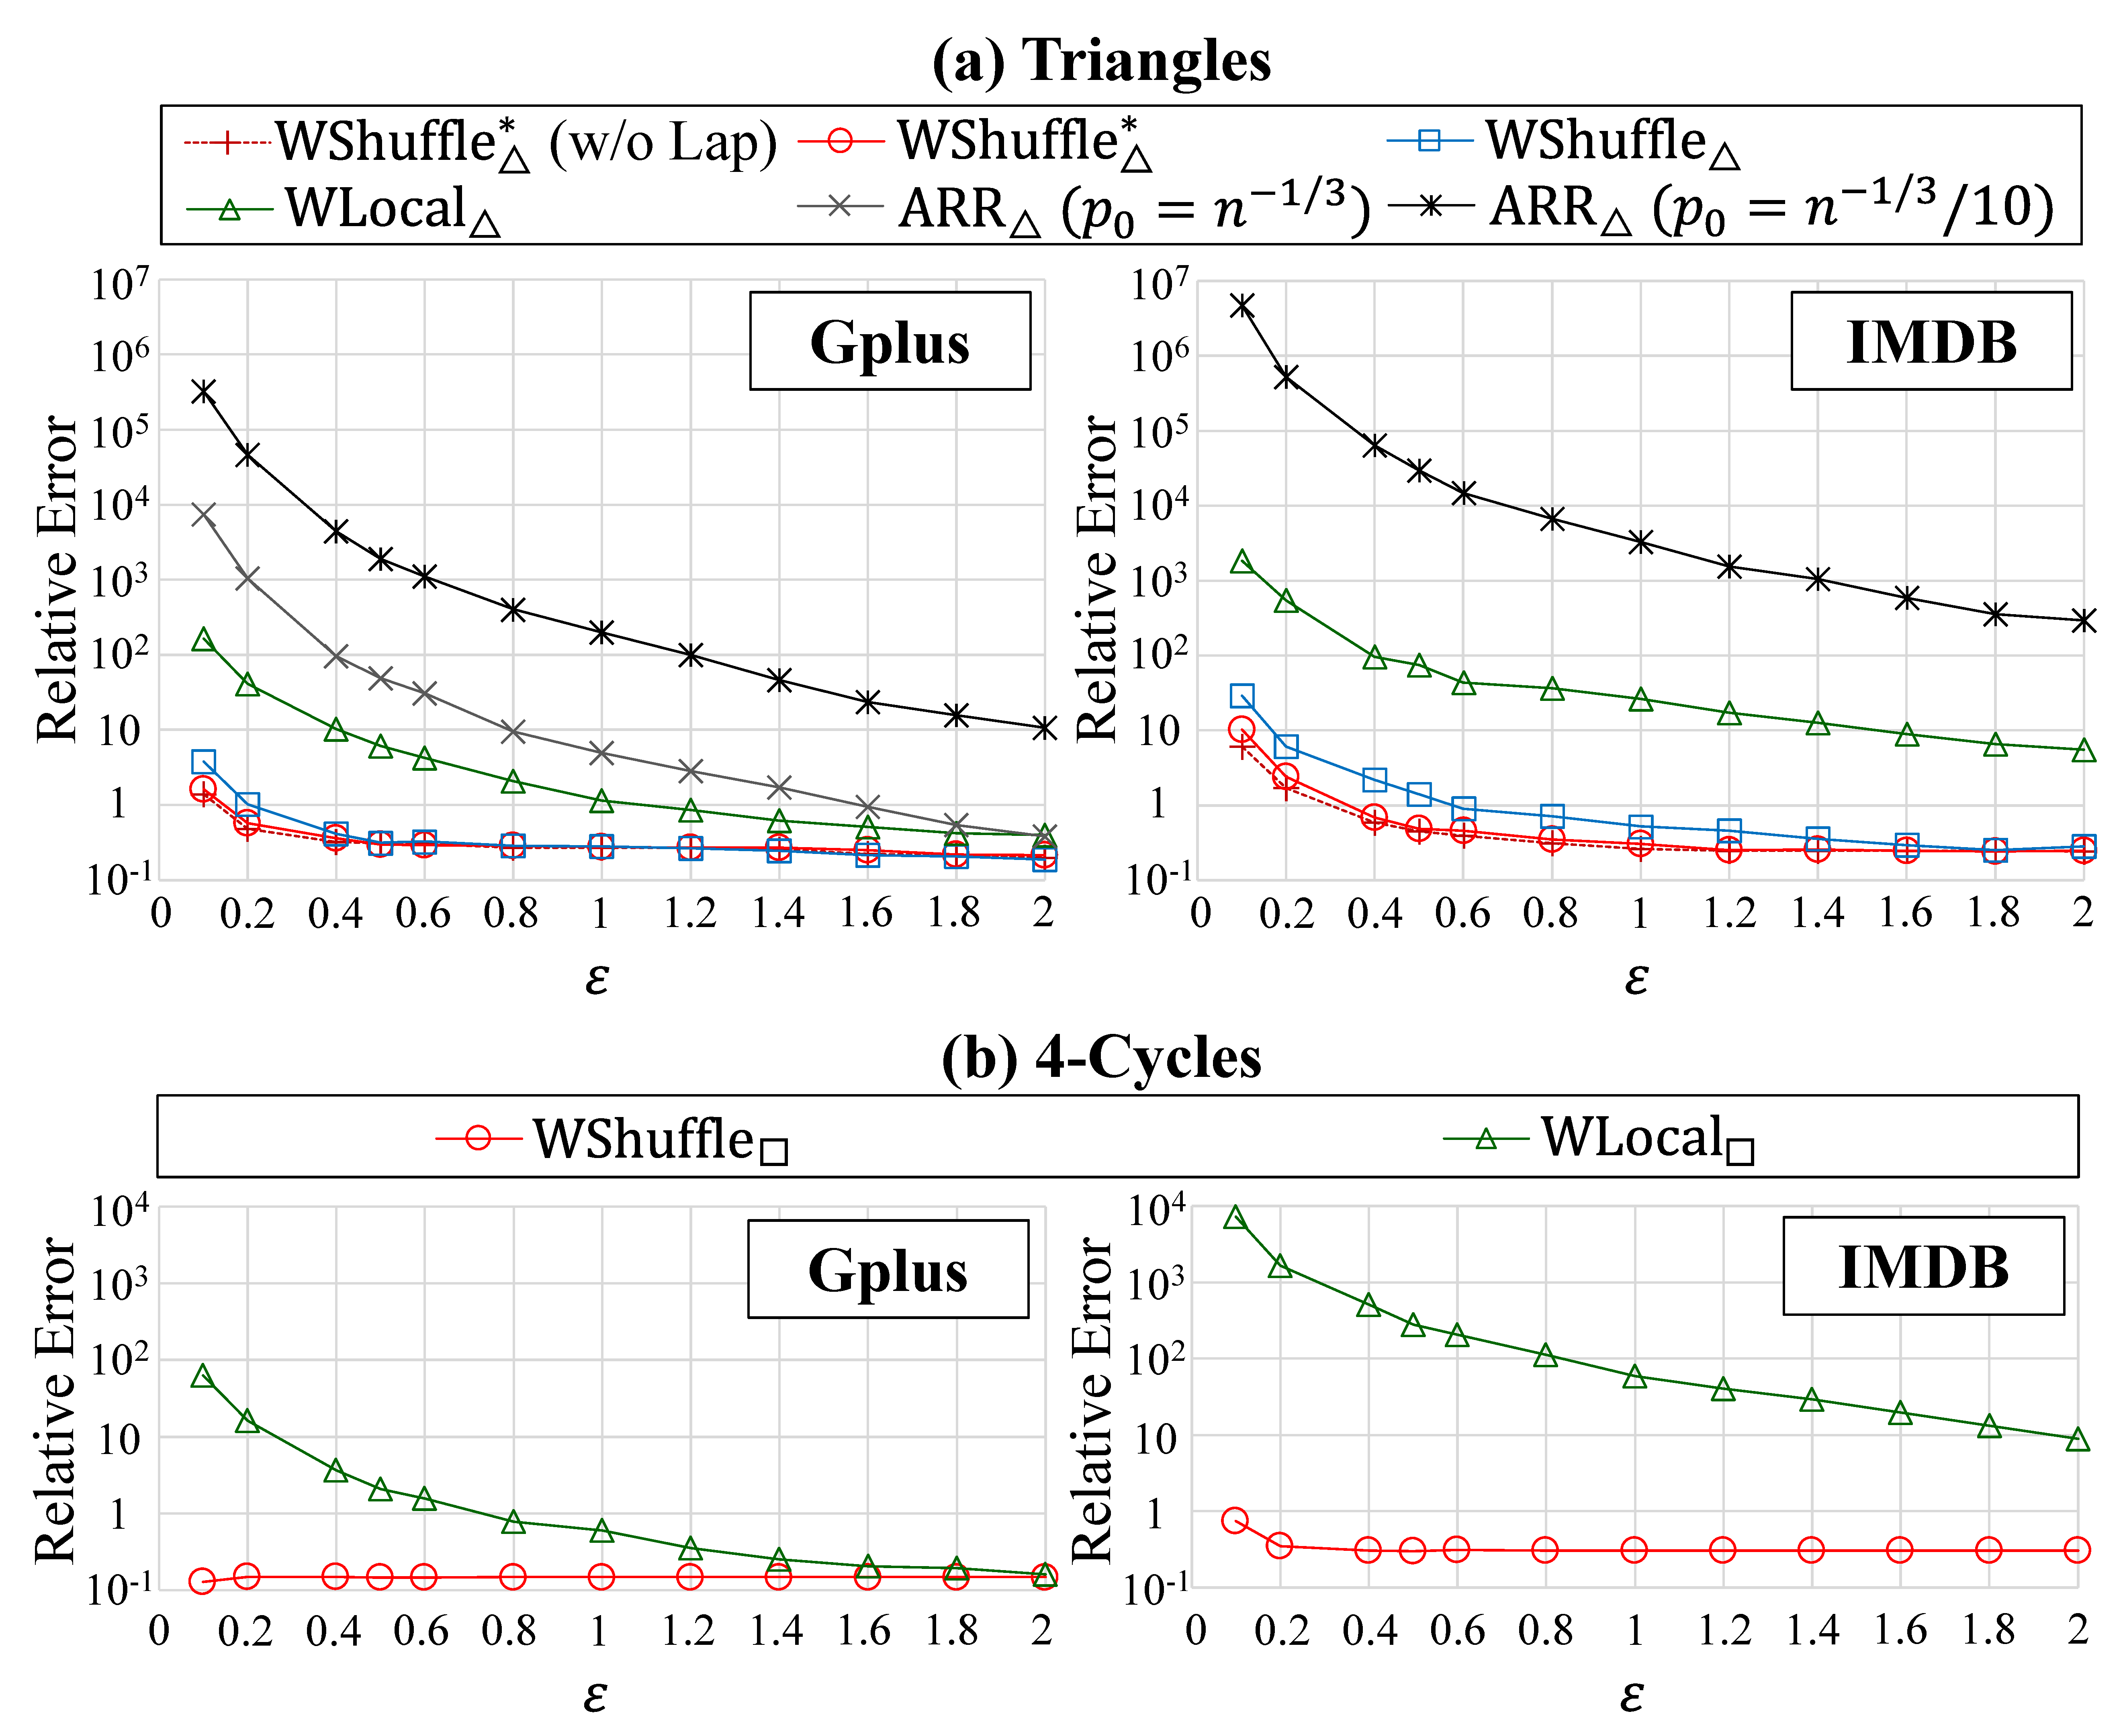
\includegraphics[width=0.99\linewidth]{fig/res1_eps.pdf}
  \vspace{-4mm}
  \caption{Relative error vs. $\epsilon$ 
  %in triangle counting 
  ($n=107614$ in \Gplus{}, $n=896308$ in \IMDB{}, $c=1$). 
  $p_0$ is the sampling probability in the ARR. 
  %; numerical bound in \cite{Feldman_FOCS21}). 
  }
  \label{chap3-fig:res1_eps}
\end{figure}

% \begin{table}[t]
%   \centering
%   (a) \Gplus{}\\
%   \begin{tabular}{|c|c|c|c|}
%     \hline
%     & \AlgWSTriVR{} & \AlgWSTri{} & \AlgWSCyc{} \\ \hline
%     $\epsilon=0.5$ & $0.298$ & $0.312$ & $0.145$ \\ \hline
%     $\epsilon=1$ & $0.277$ & $0.279$ & $0.147$ \\ \hline
%   \end{tabular}\\
%   (b) \IMDB{}\\
%   \begin{tabular}{|c|c|c|c|}
%     \hline
%      & \AlgWSTriVR{} & \AlgWSTri{} & \AlgWSCyc{} \\ \hline
%     $\epsilon=0.5$ & $0.488$ & $1.41$ & XX \\ \hline
%     $\epsilon=1$ & $0.308$ & $0.522$ & XX \\ \hline
%   \end{tabular}
%   \caption{Relative error when $\epsilon=0.5$ or $1$ ($n=107614$ in \Gplus{} and $896308$ in \IMDB{}; $c=1$). 
%   }
%   \label{chap3-tab:res1_eps_tri_0.5}
% \end{table}

\begin{table}[t]
  \caption{Relative error (RE) when $\epsilon=0.5$ or $1$ and computational time ($n=107614$ in \Gplus{}, $n=896308$ in \IMDB{}, $c=1$). 
  The lowest relative error is highlighted in bold.
  }
  \vspace{-4mm}
  \centering
%   (a) Triangle (\Gplus{})\\
  (a) \Gplus{}\\
  \begin{tabular}{|c|c|c|c|}
    \hline
    & RE ($\epsilon=0.5$) & RE ($\epsilon=1$) & Time (sec)\\ \hline
    \AlgWSTriVR{} & $\bm{2.98 \times 10^{-1}}$ & $\bm{2.77 \times 10^{-1}}$ & $3.60 \times 10^1$ \\ \hline
    \AlgWSTri{} & $3.12 \times 10^{-1}$ & $2.79 \times 10^{-1}$ & $3.62 \times 10^1$ \\ \hline
    \AlgWLTri{} & $6.10 \times 10^0$ & $1.14 \times 10^0$ & $5.83 \times 10^1$ \\ \hline
    \AlgARRTri{} ($p_0=n^{-1/3}$) & $4.90 \times 10^1$ & $4.93 \times 10^0$ & $7.15 \times 10^2$ \\ \hline
    \hspace{-0.5mm}\AlgARRTri{} ($p_0=0.1n^{-1/3}$)\hspace{-0.5mm} & $1.88 \times 10^3$ & $1.97 \times 10^2$ & $3.48 \times 10^1$ \\ \hline \hline
    \AlgWSCyc{} & $\bm{1.45 \times 10^{-1}}$ & $\bm{1.47 \times 10^{-1}}$ & $3.47 \times 10^1$ \\ \hline
    \AlgWLCyc{} & $2.08 \times 10^0$ & $5.96 \times 10^{-1}$ & $5.70 \times 10^1$ \\ \hline
  \end{tabular}\\
%   (b) Triangle (\IMDB{})\\
  (b) \IMDB{}\\
  \begin{tabular}{|c|c|c|c|}
    \hline
    & RE ($\epsilon=0.5$) & RE ($\epsilon=1$) & Time (sec)\\ \hline
    \AlgWSTriVR{} & $\bm{4.88 \times 10^{-1}}$ & $\bm{3.08 \times 10^{-1}}$ & $2.39 \times 10^3$ \\ \hline
    \AlgWSTri{} & $1.41 \times 10^0$ & $5.22 \times 10^{-1}$ & $2.40 \times 10^3$ \\ \hline
    \AlgWLTri{} & $7.46 \times 10^1$ & $2.63 \times 10^1$ & $3.96 \times 10^3$ \\ \hline
    \hspace{-0.5mm}\AlgARRTri{} ($p_0=0.1n^{-1/3}$)\hspace{-0.5mm} & $2.98 \times 10^4$ & $3.27 \times 10^3$ & $2.81 \times 10^3$ \\ \hline \hline
    \AlgWSCyc{} & $\bm{3.03 \times 10^{-1}}$ & $\bm{3.08 \times 10^{-1}}$ & $2.29 \times 10^3$ \\ \hline
    \AlgWLCyc{} & $2.82 \times 10^2$ & $5.91 \times 10^1$ & $3.91 \times 10^3$ \\ \hline
  \end{tabular}
%   (c) 4-cycle (\Gplus{})\\
%   \begin{tabular}{|c|c|c|c|}
%     \hline
%     & RE ($\epsilon=0.5$) & RE ($\epsilon=1$) & Time (sec)\\ \hline
%     \AlgWSCyc{} & $XXX$ & $XXX$ & $XXX$ \\ \hline
%     \AlgWLCyc{} & $XXX$ & $XXX$ & $XXX$ \\ \hline
%   \end{tabular}\\
  \label{chap3-tab:res1_eps_tri_time}
\end{table}

Figure~\ref{chap3-fig:res1_eps} shows the relative error ($c=1$). 
% Here, we used the numerical upper bound in \cite{Feldman_FOCS21} for $\epsilon$ in the shuffle algorithms. 
% We also 
Here, we show the performance of \AlgWSTri{} when we do not add the Laplacian noise (denoted by \AlgWSTri{} (w/o Lap)). 
In \IMDB{}, we do not show \AlgARRTri{} with $p_0 = n^{-1/3}$, because it takes too much time (longer than one day). 
Table~\ref{chap3-tab:res1_eps_tri_time} highlights the relative error when $\epsilon=0.5$ or $1$. 
It also shows the running time of counting triangles or 4-cycles when $\epsilon=1$ (we verified that the running time had little dependence on $\epsilon$). 

Figure~\ref{chap3-fig:res1_eps} and Table~\ref{chap3-tab:res1_eps_tri_time} show that our shuffle algorithms dramatically improve the local algorithms. 
% For example, 
In triangle counting, 
\AlgWSTriVR{} outperforms \AlgWLTri{} by one or two orders of magnitude and \AlgARRTri{} by even more\footnote{Note that \AlgARRTri{} uses only the lower-triangular part of the adjacency matrix $\bmA$ and therefore provides 
% $\epsilon$-edge LDP and 
$\epsilon$-edge DP (rather than $2\epsilon$-edge DP); i.e., it does not suffer from the doubling issue explained in Section~\ref{chap3-sub:privacy}. However, Figure~\ref{chap3-fig:res1_eps} shows that \AlgWSTriVR{} significantly outperforms \AlgARRTri{} 
% with the same privacy budget in edge DP.
even if we double $\epsilon$ for only \AlgWSTriVR{}.}. 
% Although the relative error of \AlgARRTri{} can be improved by using a larger $p_0$, it results in longer running time. 
\AlgWSTriVR{} also requires less running time than \AlgARRTri{} with $p_0 = n^{-1/3}$. 
Although the running time of \AlgARRTri{} can be improved by using a smaller $p_0$, it results in a higher relative error. 
% Similarly, 
In 4-cycle counting, 
\AlgWSCyc{} significantly outperforms \AlgWLCyc{}. 
The difference between our shuffle algorithms and the local algorithms is larger in \IMDB{} because it is more sparse; i.e., the difference between $d_{max}$ and $n$ is larger in \IMDB{}. 
This is consistent with our theoretical results in Tables~\ref{chap3-tab:upper_bounds_triangle} and \ref{chap3-tab:upper_bounds_4cycle}. 

Figure~\ref{chap3-fig:res1_eps} and Table~\ref{chap3-tab:res1_eps_tri_time} also show that \AlgWSTriVR{} outperforms \AlgWSTri{}, especially when $\epsilon$ is small. 
% or the dataset is sparse, i.e., \IMDB{}. 
This is because the variance is large when $\epsilon$ is small. 
In addition, \AlgWSTriVR{} significantly outperforms \AlgWSTri{} in \IMDB{} because \AlgWSTriVR{} significantly reduces the variance when $d_{max} \ll n$, as shown in Table~\ref{chap3-tab:upper_bounds_triangle}. 
In other words, this is also consistent with our theoretical results. 
For example, when $\epsilon=0.5$, our variance reduction technique reduces the relative error from $1.41$ to $0.488$ (about one-third) in \IMDB{}. 

Furthermore, Figure~\ref{chap3-fig:res1_eps} shows that the relative error of \AlgWSTriVR{} is hardly changed by adding the Laplacian noise. 
This is because the sensitivity of each user's degree $d_i$ is very small ($=1$). 
In this case, the Laplacian noise is also very small. 

\begin{figure}[t]
  \centering
  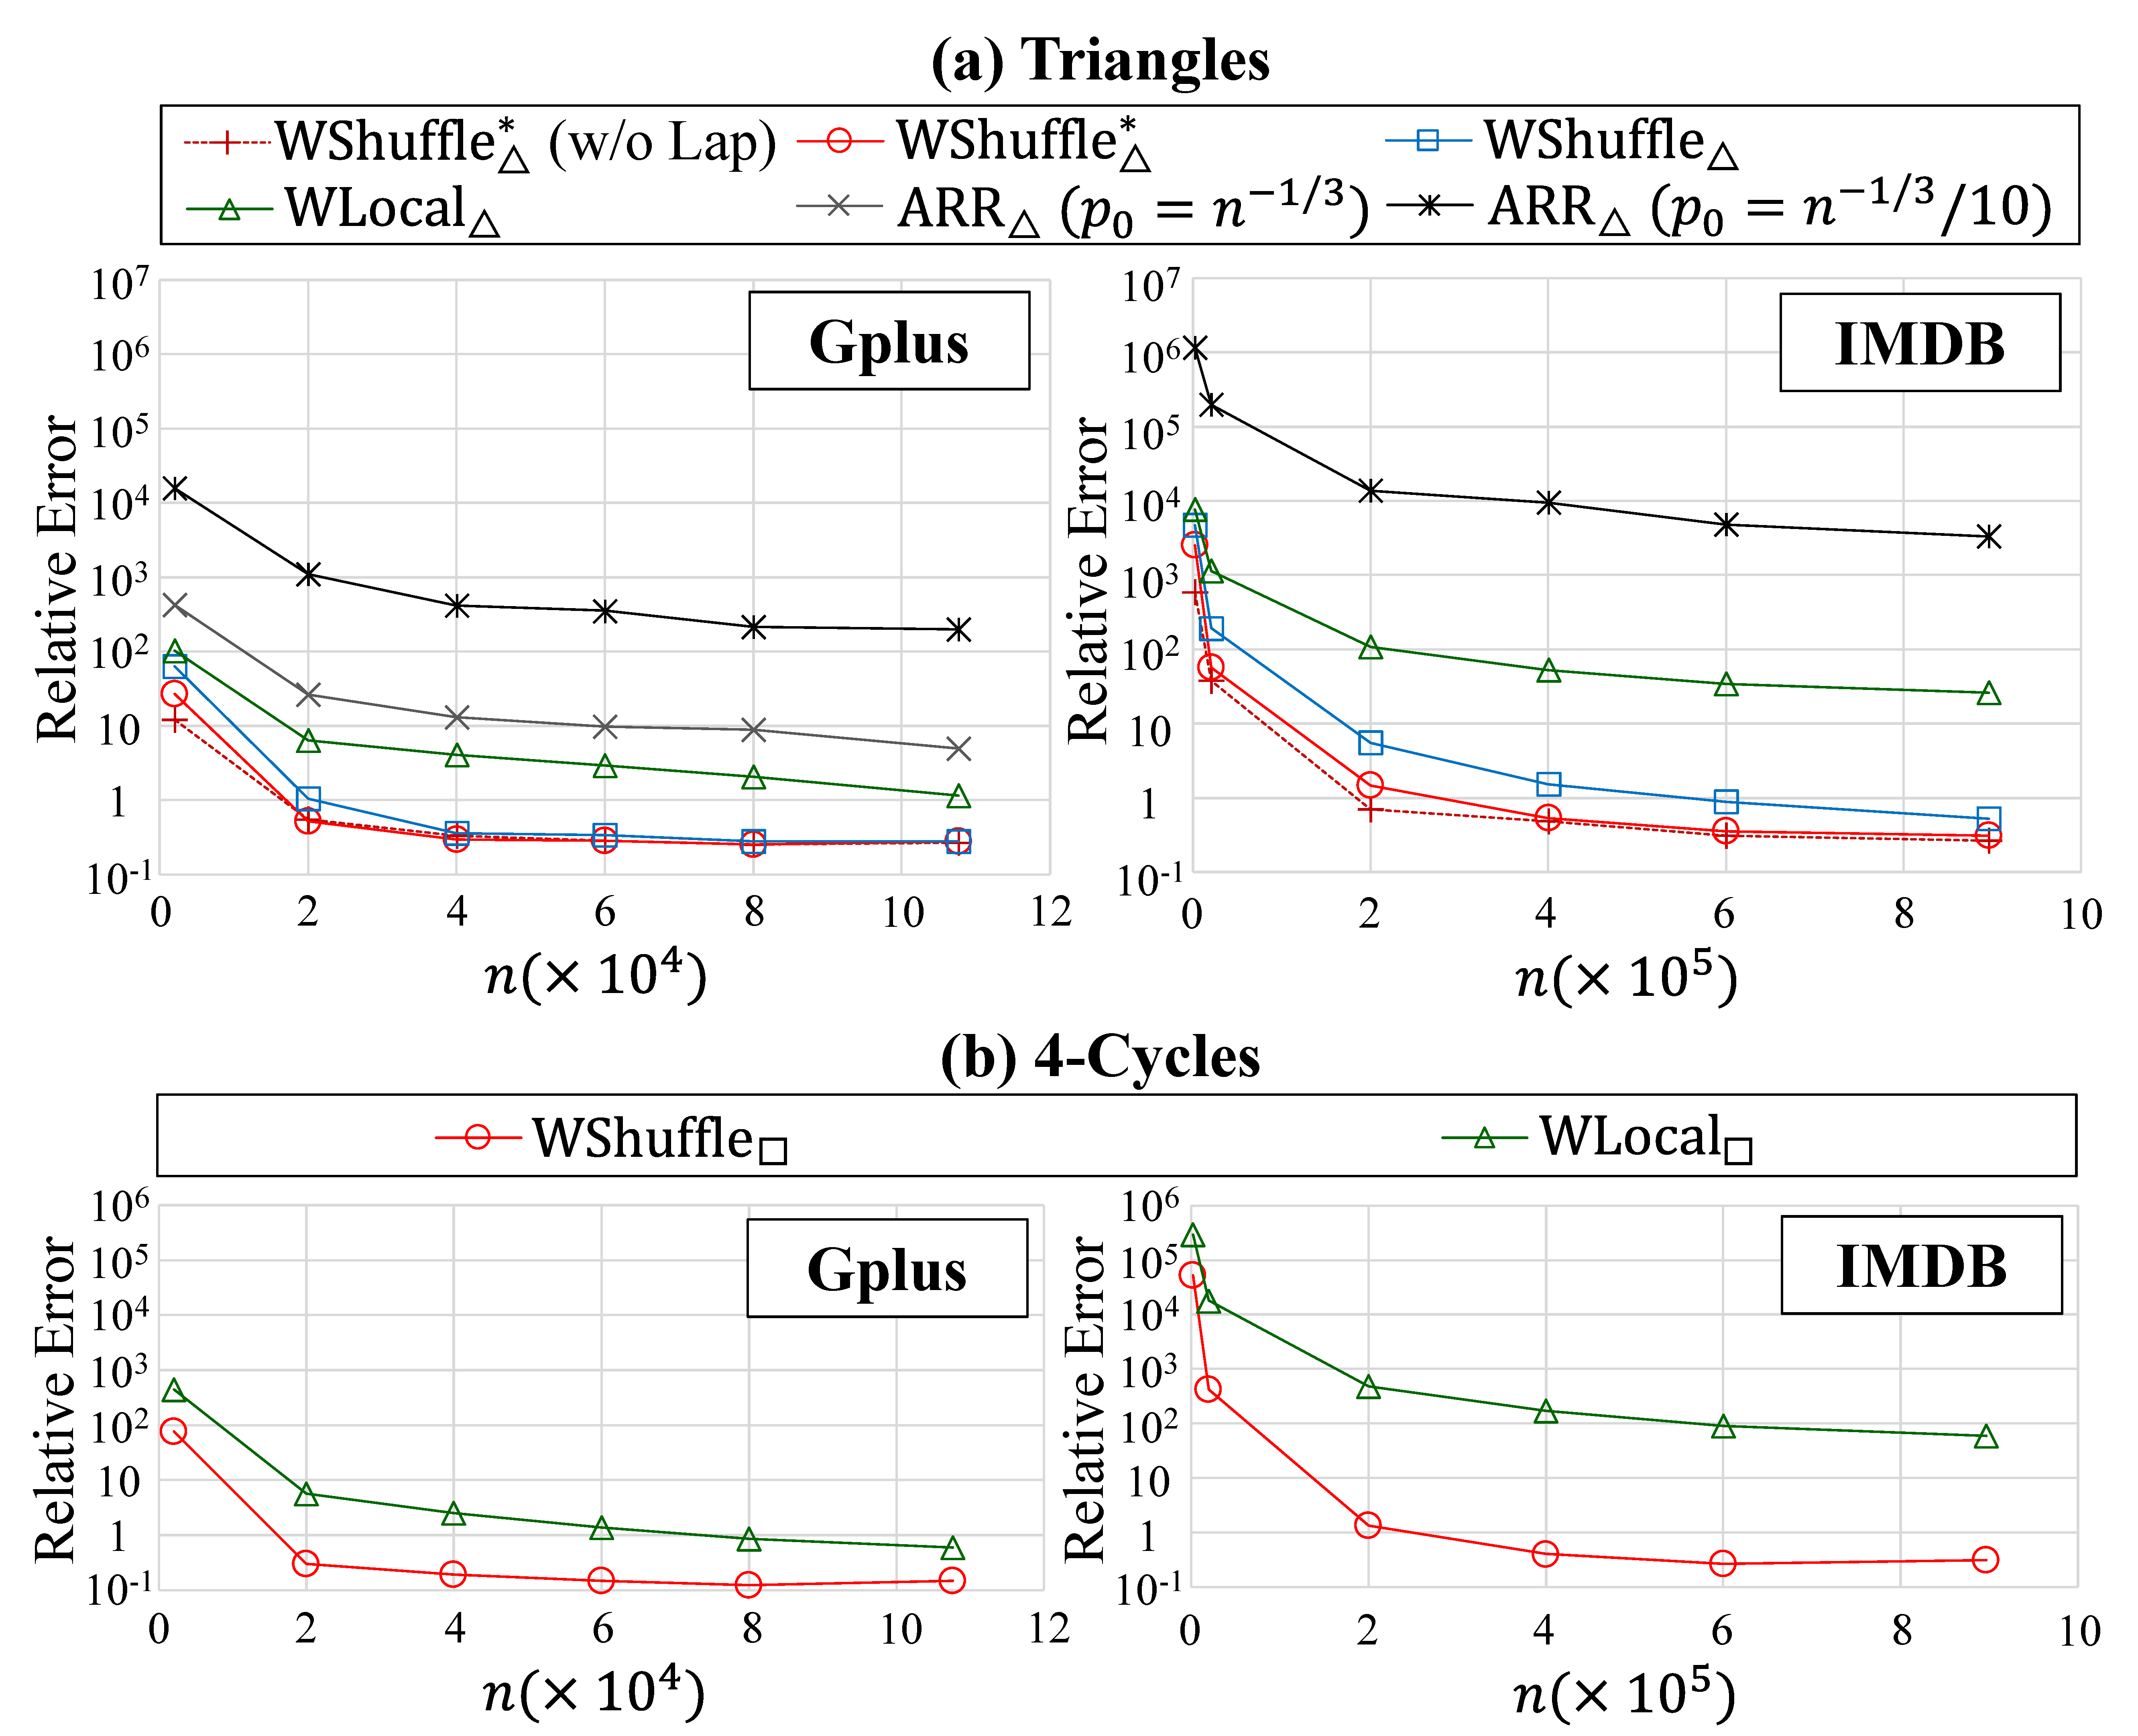
\includegraphics[width=0.99\linewidth]{fig/res2_n.pdf}
  \vspace{-4mm}
  \caption{Relative error vs. $n$ ($\epsilon=1$, $c=1$).
  }
  \label{chap3-fig:res2_n}
\end{figure}

% Table~\ref{chap3-tab:res1_eps_tri_time} shows that 
Our \AlgWSTriVR{} achieves a relative error of $0.3$ ($\ll 1$) 
% and \AlgWSCyc{} achieve relative errors of $0.15$ to $0.3$ ($\ll 1$) 
% with a reasonable privacy budget -- $\epsilon = 0.5$ or $1$ in element DP and $2\epsilon = 1$ or $2$ in edge DP. 
when the privacy budget is $\epsilon = 0.5$ or $1$ in element DP ($2\epsilon = 1$ or $2$ in edge DP). 
\AlgWSCyc{} achieve a relative error of $0.15$ to $0.3$ with a smaller privacy budget (e.g., $\epsilon = 0.2$) because it  does not send local edges -- the error of \AlgWSCyc{} is mainly caused by user-pair sampling that is independent of $\epsilon$. 

In summary, our \AlgWSTriVR{} and \AlgWSCyc{} significantly outperform the local algorithms and achieve a relative error much smaller than $1$ with a reasonable privacy budget, i.e., $\epsilon \leq 1$. 

\smallskip
\noindent{\textbf{Relative Error vs. $n$.}}~~Next, we evaluated the relation between the relative error and $n$. 
% the number $n$ of users. 
Specifically, we randomly selected $n$ users from all users and extracted a graph with $n$ users. 
Then we set $\epsilon = 1$ and changed $n$ to various values starting from $2000$. 
%from $2000$ to $107614$ and $896308$ in \Gplus{} and \IMDB{}, respectively. 

Figure~\ref{chap3-fig:res2_n} shows the results ($c=1$). 
% We observe that 
When $n=2000$, \AlgWSTri{} and \AlgWSCyc{} provide 
%almost the same relative error as 
relative errors close to \AlgWLTri{} and \AlgWLCyc{}, respectively. 
This is because the privacy amplification effect is limited when $n$ is small. 
For example, when $n=2000$ and $\epsilon=1$, 
% and $\delta=10^{-8}$, 
the numerical bound is $\epsilon_L=1.88$. 
The value of $\epsilon_L$ increases with increase in $n$; e.g., when $n=107614$ and $896308$, the numerical bound is $\epsilon_L= 5.86$ and $7.98$, respectively. 
This explains the reason that our shuffle algorithms significantly outperform the local algorithms when $n$ is large in Figure~\ref{chap3-fig:res2_n}. 
% the large difference between our shuffle algorithms and the local algorithms. 
% in Figure~XX. 

% Figure~XX also shows that the relative error decreases with increase in $n$. 
% There are two reasons for this: (i) the squares of the true triangle and 4-cycle counts are $O(n^2 d_{max}^4)$ and $O(n^2 d_{max}^6)$, respectively; (ii) $d_{max}$ is proportional to $n$, as we randomly selected $n$ users from all users. 


% \smallskip
% \noindent{\textbf{Clustering Coefficient.}}~~TBD

\smallskip
\noindent{\textbf{Parameter $c$ in \AlgWSTriVR{}.}}~~Finally, we evaluated our \AlgWSTriVR{} while changing the parameter $c$ that controls the bias and variance. 
% of the estimate. 
Recall that as $c$ increases, the bias is increased, and the variance is reduced. 
We set $\epsilon=0.1$ or $1$ and changed $c$ from $0.1$ to $4$. 

Figure~\ref{chap3-fig:res4_thr} shows the results. 
Here, we also show the relative error of \AlgWSTri{}. 
We observe that the optimal $c$ is different for $\epsilon=0.1$ and $\epsilon=1$. The optimal $c$ is around $3$ to $4$ for $\epsilon=0.1$, whereas the optimal $c$ is around $0.5$ to $1$ for $\epsilon=1$. 
This is because the variance of \AlgWSTri{} is large (resp.~small) when $\epsilon$ is small (resp.~large). 
For a small $\epsilon$, a large $c$ is effective in significantly reducing the variance. 
For a large $\epsilon$, a small $c$ is effective in keeping a small bias. 
% The optimization of $c$ in \AlgWSTriVR{} is an interesting future research direction. 

We also observe that \AlgWSTriVR{} is always better than (or almost the same as) \AlgWSTri{} when $c=1$ or $2$. 
This is because most users' degrees are smaller than the average degree $d_{avg}$, as described in Section~\ref{chap3-sub:var_red}. 
When $c=1$ or $2$, most user-pairs are ignored. 
Therefore, we can significantly reduce the variance at the cost of a small bias. 

\begin{figure}[t]
  \centering
  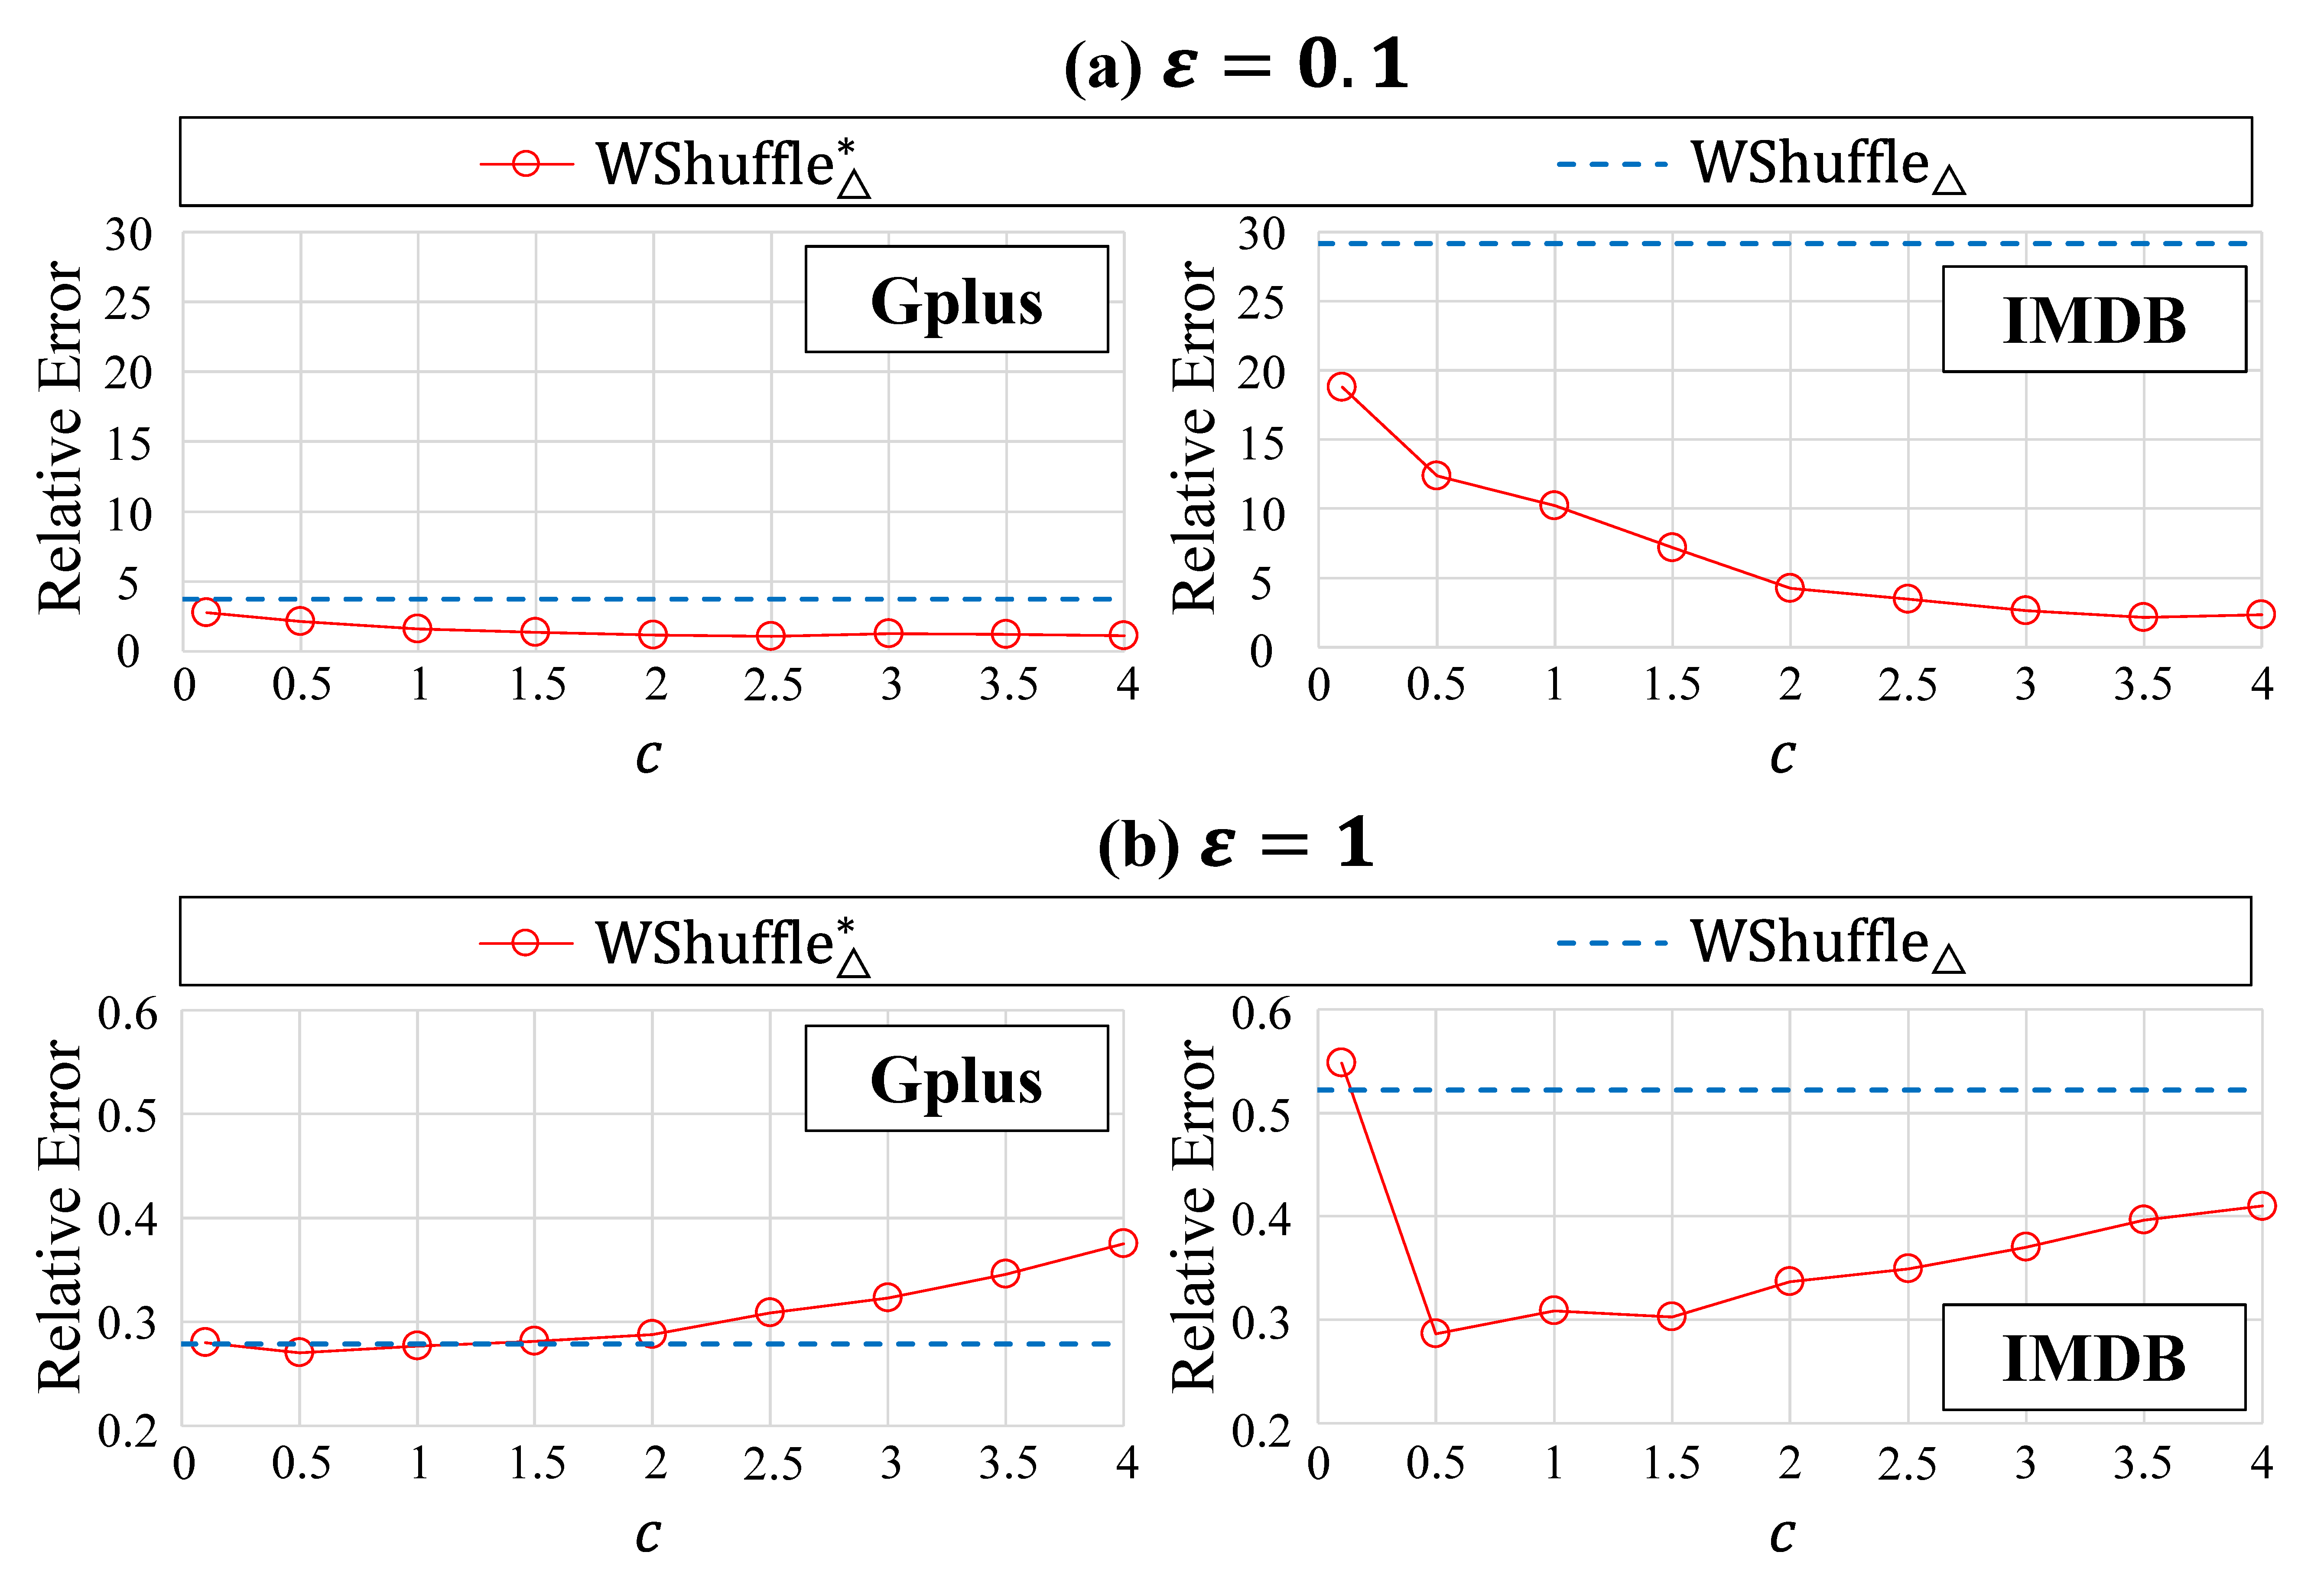
\includegraphics[width=0.99\linewidth]{fig/res4_thr.pdf}
  \vspace{-4mm}
  \caption{Relative error vs. parameter $c$ in \AlgWSTriVR{} ($n=107614$ in \Gplus{}, $n=896308$ in \IMDB{}).
  }
  \label{chap3-fig:res4_thr}
\end{figure}

\smallskip
\noindent{\textbf{Summary.}}~~In summary, our answers to the three questions at the beginning of Section~\ref{chap3-sec:experiments} are as follows. 
RQ1: Our \AlgWSTriVR{} and \AlgWSCyc{} outperform the one-round local algorithms by one or two orders of magnitude (or even more). 
% \AlgWSTriVR{} is even comparable to the two-rounds local algorithm in \cite{Imola_USENIX22} (\AlgTwoRS{}) that requires a lot of user effort 
% and synchronization 
% in terms of accuracy. 
RQ2: Our variance reduction technique significantly reduces the relative error (e.g., by about one-third) 
for a small $\epsilon$ in a sparse dataset. 
% when $\epsilon$ is small or the dataset is sparse. 
RQ3: 
% Our \AlgWSTriVR{} and \AlgWSCyc{} achieve a relative error of $0.15$ to $0.3$ ($\ll 1$) when $\epsilon=0.5$ or $1$ in element DP ($2\epsilon=1$ or $2$ in edge DP). 
\AlgWSTriVR{} achieves a relative error of $0.3$ ($\ll 1$) when $\epsilon=0.5$ or $1$ in element DP ($2\epsilon=1$ or $2$ in edge DP). 
\AlgWSCyc{} achieves a relative error of $0.15$ to $0.3$ with a smaller privacy budget: $\epsilon=0.2$. 

\section{Conclusion}
\label{chap3-sec:conclusion}
In this paper, we made the first attempt (to our knowledge) to 
shuffle graph data for privacy amplification. 
% apply the shuffle model to graph data. 
We proposed wedge shuffling as a basic technique and then applied it to 
% to enable the privacy amplification of graph data. 
% Then we proposed 
one-round triangle and 4-cycle counting with several additional techniques. 
% algorithms based on wedge shuffling. 
We showed upper bounds on 
% the expected $l_2$ loss 
the MSE 
for each algorithm. 
We also showed through comprehensive experiments that our one-round shuffle algorithms significantly outperform the one-round local algorithms and achieve a small relative error with a reasonable privacy budget, e.g., smaller than $1$ in edge DP. 

For future work, we would like to apply wedge shuffling to other subgraphs such as 3-hop paths \cite{Sun_CCS19} and $k$-triangles \cite{Karwa_PVLDB11}. 


